\documentclass[11pt,a4paper]{report}

% REMAINING TODO SELF
% Adust the 2 Python generation files with an abstract file for clarity
% Assuming I get the Apple device in time, I will also benchmark the optimised MEDS implementation on that CPU. Explore the speedup possibilities on other ARM-based CPUs (such as Apple M1) which can utilize larger caches and/or the better KECCAK primitives possible on Armv8.2-A (Cortex-A72 uses Armv8-A). See: \url{https://developer.arm.com/documentation/100076/0100A64-Instruction-Set-Reference/A64-Cryptographic-AlgorithmsA64-Cryptographic-instructions?lang=en}

\usepackage[table]{xcolor}
\definecolor{linkcolor}{rgb}{0.65,0,0}
\definecolor{citecolor}{rgb}{0,0.65,0}
\definecolor{urlcolor}{rgb}{0,0,0.65}

\usepackage[chapter]{algorithm}
\usepackage[noend]{algpseudocode}
\usepackage{algpseudocode}
\usepackage{amsmath}
\usepackage{amssymb}
\usepackage{amsthm}
\usepackage{array}
\usepackage[english]{babel}
\usepackage{booktabs}
\usepackage{dsfont}
\usepackage{enumitem}
\usepackage{etoolbox}
\usepackage[a4paper]{geometry}
\usepackage{graphics}
\usepackage{graphicx}
\usepackage[utf8]{inputenc}
\usepackage{listings}
\usepackage{mdframed}
\usepackage{microtype}
\usepackage{multirow}
\usepackage{natbib}
\usepackage{parskip}
\usepackage{pgf-pie}
\usepackage{tabularx}
\usepackage{todonotes}
\usepackage{url}
\usepackage{xurl}

\usepackage[colorlinks=true, backref=page, linkcolor=linkcolor, urlcolor=urlcolor, citecolor=citecolor]{hyperref}

\interfootnotelinepenalty=10000
\widowpenalty=10000
\clubpenalty=10000

% Define nice pie chart colors
% \definecolor{pie1}{HTML}{03045e}
% \definecolor{pie2}{HTML}{023e8a}
% \definecolor{pie3}{HTML}{0077b6}
% \definecolor{pie4}{HTML}{0096c7}
% \definecolor{pie5}{HTML}{00b4d8}
% \definecolor{pie6}{HTML}{48cae4}
% \definecolor{pie7}{HTML}{90e0ef}
% \definecolor{pie8}{HTML}{ade8f4}
% \definecolor{pie9}{HTML}{caf0f8}

\setlength{\marginparwidth}{2cm}
% \hypersetup{
%     colorlinks,
%     citecolor=black,
%     filecolor=black,
%     linkcolor=black,
%     urlcolor=black
% }

\theoremstyle{definition}
\newmdtheoremenv{definition}{Definition}[section]
\AtBeginEnvironment{definition}{\vspace{1em}}

\AtBeginEnvironment{tabular}{\vspace{0.5em}}

\newcolumntype{R}[1]{>{\raggedleft\arraybackslash}p{#1}}

\lstdefinestyle{CStyle}{
  language=C,
  commentstyle=\color{green!60!blue},
  keywordstyle=\color{blue},
  numberstyle=\tiny\color{black!80},
  stringstyle=\color{green},
  basicstyle=\footnotesize\ttfamily,
  breakatwhitespace=false,         
  breaklines=true,                 
  captionpos=b,                    
  keepspaces=true,                 
  numbers=left,                    
  numbersep=5pt,                  
  showspaces=false,                
  showstringspaces=false,
  showtabs=false,                  
  tabsize=2,
  morekeywords={uint64_t, pmod_mat_entry, uint16x4_t, uint16x8_t, uint32x4_t, uint64x2_t, vmull_u32, vget_low_u32, vmull_high_u32, vuzp2q_u32, vshrq_n_u32, vmlsq_u32, vcgeq_u16, vandq_u16, vsubq_u16, vmovn_u32, pmod_mat_t, pmod_mat_vec_t, pmod_mat_vec_w_t, ZERO_VEC_W, MUL_ACC_VEC, FREEZE_REDUCE_VEC, MUL_ACC_VEC_LOW, REDUCE_VEC_32BIT, COMBINE_VEC}
}


\lstdefinestyle{ASMStyle}{
  language=C,
  commentstyle=\color{green!60!blue},
  keywordstyle=\color{blue},
  numberstyle=\tiny\color{black!80},
  stringstyle=\color{green},
  basicstyle=\footnotesize\ttfamily,
  breakatwhitespace=false,         
  breaklines=true,                 
  captionpos=b,                    
  keepspaces=true,                 
  numbers=left,                    
  numbersep=5pt,                  
  showspaces=false,                
  showstringspaces=false,
  showtabs=false,                  
  tabsize=2,
  morekeywords={umull, umull2, uzp2, ushr, mls, xtn, cmhs, and, sub, mul, umlal}
}

% Set the line spacing between paragraphs
% \setlength{\parskip}{1em}
% Remove paragraph indentation
% \setlength{\parindent}{0pt}

% URL LINE BREAKS
\expandafter\def\expandafter\UrlBreaks\expandafter{\UrlBreaks% save the current one
  \do\a\do\b\do\c\do\d\do\e\do\f\do\g\do\h\do\i\do\j%
  \do\k\do\l\do\m\do\n\do\o\do\p\do\q\do\r\do\s\do\t%
  \do\u\do\v\do\w\do\x\do\y\do\z\do\A\do\B\do\C\do\D%
  \do\E\do\F\do\G\do\H\do\I\do\J\do\K\do\L\do\M\do\N%
  \do\O\do\P\do\Q\do\R\do\S\do\T\do\U\do\V\do\W\do\X%
  \do\Y\do\Z\do\*\do\-\do\~\do\'\do\"\do\-}%

\makeatletter %otherwise geometry resets everything
\Gm@restore@org
\makeatother

\setlength{\itemsep}{0cm}
\setlength{\voffset}{0cm}
\setlength{\headheight}{0cm}
\setlength{\topmargin}{0cm}

\graphicspath{{imgs/}}

\begin{document}
\begin{titlepage}
  \begin{center}
    \textsc{\LARGE Master Thesis\\Computing Science}\\[1.5cm]
    
\includegraphics[height=100pt]{logo}

    \vspace{0.4cm}
    \textsc{\Large Radboud University}\\[1cm]
    \hrule
    \vspace{0.4cm}
    \textbf{\huge Optimizing the MEDS Implementation for ARMv8}\\[0.4cm]
    \vspace{0.2cm}
    \hrule
    \vspace{2cm}
    \begin{minipage}[t]{0.45\textwidth}
      \begin{flushleft} \large
        \textit{Author:}\\
        Lars Jeurissen\\
        s1022856\\
        \texttt{\href{mailto:lars.jeurissen@ru.nl}{lars.jeurissen@ru.nl}}
      \end{flushleft}
    \end{minipage}
    \begin{minipage}[t]{0.45\textwidth}
      \begin{flushright} \large
        \textit{First supervisor/assessor:}\\
        prof. dr. Peter Schwabe\\
        \texttt{\href{mailto:peter@cryptojedi.org}{peter@cryptojedi.org}}\\[1.3cm]
        \textit{Second supervisor:}\\
        dr. Simona Samardjiska\\
        \texttt{\href{mailto:simonas@cs.ru.nl}{simonas@cs.ru.nl}}
      \end{flushright}
    \end{minipage}
    \vfill
    {\large \today}
  \end{center}
\end{titlepage}

% \renewcommand{\abstractname}{Acknowledgements}
\begin{abstract}
Thank you.
\end{abstract}

\renewcommand{\abstractname}{Abstract}
\begin{abstract}
Abstract.

%The abstract of your thesis is a brief description of the research hypothesis,
%scientific context, motivation, and results.
%The preferred size of an abstract is one paragraph or one page of text.
\end{abstract}


\hypersetup{linkcolor=black}
\tableofcontents
\hypersetup{linkcolor=linkcolor}

\newpage

\chapter{Introduction}
\label{ch:introduction}

\section{Context}
As the research on quantum computers progresses, we are getting increasingly closer to the point where quantum computers will be able to utilize algorithms such as Shor's algorithm~\cite{shor1994algorithms} and Grover's algorithm~\cite{grover1996fast} to break various cryptographic schemes, causing the absolute collapse of the present public key algorithms that are considered secure~\cite{mavroeidis2018impact}. As the majority of the digital world relies on the security of these cryptographic schemes, this will have devastating consequences for the security of not only the internet, but also financial transactions, secure communication, and many other critical sectors.

The solution to this problem lies in the development of cryptographic schemes that are secure against quantum computers. Such algorithms have been around for a long time, but this area of research has experienced a boost in attention ever since the National Institute of Standards and Technology (NIST) started the post-quantum cryptography (PQC) standardization process in 2017~\cite{nist2017pqc}. The goal of this process is to standardize cryptographic schemes that are secure against quantum computers.

In 2022, NIST announced the set of selected PQC algorithms, which included three digital signature schemes: CRYSTALS-Dilithium~\cite{ducas2018crystals}, Falcon~\cite{fouque2018falcon}, and SPHINCS$^+$~\cite{bernstein2015sphincs}. As two of these schemes are based on structured lattices, NIST announced a second competition in the PQC standardization process, which aims to find additional general-purpose signature schemes that are not based on structured lattices. One of the candidates in this competition is Matrix Equivalence Digital Signature (MEDS)~\cite{chou2023take}. MEDS is a code-based digital signature scheme based on the notion of Matrix Code Equivalence. In this thesis, we aim to optimize the performance of the MEDS implementation for the ARMv8 architecture.

\section{Motivation}
The need for digital signature schemes that are secure against quantum computers is increasing. Of course, the security of these schemes is the most important aspect, but the speed at which an implementation can create or verify a signature is also important. The speed of a digital signature scheme is essential for many applications, such as TLS/SSL certificate verification, electronic payments, and blockchain transactions.

Although the MEDS scheme is actively being optimized in terms of key and signature sizes, the performance of the scheme is still lacking. The reported signature verification times are in the order of hundreds of milliseconds and sometimes even seconds, depending on the security level and the chosen parameters. Traditional digital signature schemes such as RSA~\cite{rivest1978method} and ECDSA~\cite{johnson2001elliptic} can verify thousands of signatures per second on both modern and even older hardware~\cite{de1998performance,koppl2021performance}. The new post-quantum digital signature schemes must eventually achieve similar performance levels.

The two most widely used CPU architectures in the world are x86 (used in Intel and AMD processors) and ARM. ARM is used in a wide variety of devices, for example,
\begin{itemize}
  \item mobile devices and tablets such as the Apple iPhone and iPad, Samsung Galaxy, and Google Pixel;
  \item embedded and Internet of Things (IoT) devices such as smart light bulbs, smart thermostats, and smart doorbells;
  \item Apple M1/M2/M3 chips used in Apple MacBooks.
\end{itemize}
Optimizing the MEDS implementation for the ARMv8 architecture will improve the MEDS performance for these devices, as well as provide valuable insights into the performance of MEDS on ARMv8.

\section{Scope}
The goal of this thesis is to optimize the performance of the MEDS implementation for the ARMv8 architecture to the extent that further optimizations are either infeasible or provide only minimal performance improvements. To achieve this goal, we investigate the following research questions:
\begin{itemize}[left=35pt,labelsep=15pt]
  \item[RQ I.] How is CPU time distributed across the code of the MEDS implementation?
  \item[RQ II.] What optimizations can be made to improve the performance of the MEDS implementation for the ARMv8 architecture?
        \begin{itemize}
          \item[a)] Which of these optimizations can be used in general for any
                architecture?
        \end{itemize}
        % \item[RQ III.] How does the optimized MEDS implementation compare to (optimized) implementations of other digital signature schemes?
\end{itemize}

Since the submission of the original MEDS implementation to the NIST PQC competition in 2023~\cite{chou2023meds}, the authors have proposed several optimizations to the scheme to reduce the size of the public key and the signatures~\cite{chou2024reducing}. The authors have provided a new reference implementation for MEDS that implements these optimizations. In this thesis, we focus on optimizing this new implementation for the ARMv8 architecture. There are two main reasons for this focus:
\begin{itemize}
  \item Research has been done on the optimization of the original MEDS implementation for the x86 architecture (using AVX512 instructions) in~\cite{IIS2023HighLevel, IIS2023LowLevel}. Although the ARMv8 architecture is different and an optimization of the original implementation for ARMv8 would be interesting, we believe that optimizing the new implementation provides better insights into the performance of a state-of-the-art MEDS implementation.
  \item The new MEDS variant has quite a few differences compared to the original, but the core structure and algorithms remain the same. This suggests that the optimizations that we make for the new implementation can also be applied to the original implementation, should the need arise.
\end{itemize}
In this thesis, when talking about the MEDS implementation, we refer to the new reference implementation that was provided by the authors in~\cite{chou2024reducing}, unless stated otherwise.

\section{Related work}
\todo[inline]{Fix.. (en contributions?)}
Digital signature schemes and their optimization have been the subject of many research papers over the last few decades. Traditional widely-used digital signature schemes such as RSA~\cite{rivest1978method}, ECDSA~\cite{johnson2001elliptic}, and EdDSA~\cite{bernstein2012high} have received optimizations for various versions of ARM CPUs over the years~\cite{talal2009efficient,tanik2001ecdsa,xu2001efficient}. The introduction of NEON~\cite{ARMv8A-ProgrammersGuide} (ARM's SIMD instruction set) in ARMv7 has led to a new wave of optimizations for traditional digital signature schemes based on NEON instructions, starting with the work of Bernstein and Schwabe in 2011~\cite{bernstein2012neon}. This work has been continued for both symmetric and asymmetric cryptographic algorithms over the years~\cite{azarderaksh2015neon,gouvea2015implementing,seo2016efficient,seo2014parallel,wang2015higher}.

The introduction of the NIST post-quantum cryptography standardization process in 2016 has led to the development of many new public key encryption (PKE), key encapsulation mechanism (KEM), and digital signature schemes that are believed to be secure against quantum computers. Research into the NEON optimization of PKE/KEM schemes soon followed~\cite{nguyen2021fast,nguyen2021optimized,ortiz2022evaluation,streit2018post}. The optimization of post-quantum digital signature schemes has mostly focused on finalists of the competition: CRYSTALS-Dilithium~\cite{ducas2018crystals}, Falcon~\cite{fouque2018falcon}, SPHINCS$^+$~\cite{bernstein2015sphincs}, and Rainbow~\cite{ding2005rainbow} have received NEON-based optimizations for ARMv8 CPUs~\cite{becker2021neon,becker2022hybrid,kim2022accelerating,kim2022crystals,kwon2023look,nguyen2023fast}.

Besides the use of NEON instructions, the use of already optimized algorithms can greatly improve the performance of a cryptographic scheme. Common cryptographic building blocks such as the KECCAK permutation~\cite{bertoni2013keccak} and Montgomery multiplication~\cite{montgomery1985modular} have already been optimized for various ARM CPUs~\cite{becker2022hybrid,bos2014montgomery,seo2015montgomery} and are used in many digital signature schemes.

\section{Contributions}
This thesis makes the following contributions:
\begin{itemize}
  \item We provide a detailed profiling of the MEDS implementation for the ARMv8 architecture, which gives insights into the performance bottlenecks of the implementation. These profiling results, although specific to the ARMv8 architecture, can be used as a guideline for optimizing the MEDS implementation for other architectures.
  \item We provide two mutually exclusive optimizations for the MEDS implementation: a low-level optimization that focuses on the optimization of underlying functions such as matrix multiplication and the matrix systemizer, and a high-level optimization that focuses on the parallelization of the commitment loop in the signature and verification algorithms.
  \item We provide novel assembly implementations of essential functions such as modular reduction and matrix multiplication that are optimized for the ARMv8 architecture. These implementations can be used in other cryptographic schemes that require similar functions.
  \item We propose a change to the MEDS scheme that allows for larger parallelizability in the hashing process. This change provides a small speedup of both signature generation and verification.
  \item We present the benchmarking results of the optimized MEDS implementation and compare these results to the reference implementation.
  \item We compare MEDS to similar digital signature schemes in terms of performance and show that the optimized MEDS implementation is competitive with these schemes.
\end{itemize}

\section{Outline}
In Chapter~\ref{ch:preliminaries}, we provide the necessary background information on the functioning of MEDS and the specific details of the ARMv8 architecture. In Chapter~\ref{ch:profiling}, we discuss the profiling techniques that we use to obtain an understanding of the performance of MEDS and present the profiling results of the MEDS implementation. Following that, in Chapter~\ref{ch:methodology}, we discuss the optimization techniques that we use to optimize the MEDS implementation. In Chapter~\ref{ch:results}, we present and discuss the benchmarking and profiling results of our optimizations. We conclude the thesis in Chapter~\ref{ch:conclusion}, where we reflect on the results that we obtained. Finally, we discuss the remaining future work in Chapter~\ref{ch:futurework}.

All code used in this thesis is available on GitHub for reference under the GPL-3.0 license.\footnote{\url{https://github.com/MeItsLars/MEDS-ARMv8-optimization-thesis}}

% \chapter{Research Objectives}
% \label{ch:researchobjectives}
% \section{Research questions}
% The goal of this thesis is to optimize the performance of the MEDS implementation for the ARMv8 architecture to the extent that further optimizations are either infeasible or provide only minimal performance improvements. To achieve this goal, we investigate the following research questions:
% \begin{itemize}[left=35pt,labelsep=15pt]
%   \item[RQ I.] How is CPU time distributed across the code of the MEDS implementation?
%   \item[RQ II.] What optimizations can be made to improve the performance of the MEDS implementation for the ARMv8 architecture?
%   \begin{itemize}
%     \item[a)] Which of these optimizations can be used in general for any 
%     architecture?
%   \end{itemize}
%   \item[RQ III.] How does the optimized MEDS implementation compare to (optimized) implementations of other digital signature schemes?
% \end{itemize}

\chapter{Preliminaries}
\label{ch:preliminaries}
In this chapter, we provide the relevant background concepts on the functioning of the MEDS scheme, the ARMv8 architecture, the optimization of cryptographic schemes and modular reduction. Additionally, we give a small overview of the notations that we use in this thesis.

\section{Notations}
\label{sec:notations}
In the MEDS scheme and this thesis, we use the following notations:
\begin{itemize}
  \item $\mathbb{F}_q$: The finite field of size $q$.
  \item $\mathbb{F}_q^{m \times n}$: The set of matrices of size $m \times n$ ($m$ rows and $n$ columns) over $\mathbb{F}_q$, meaning that each element of the matrix is an element of $\mathbb{F}_q$.
  \item $\text{GL}_k(q)$: The set of all invertible $k \times k$ matrices over $\mathds{F}_q$.
  \item $\textbf{A} \in \mathbb{F}_q^{m \times n}$: A matrix $\textbf{A}$ of size $m \times n$ over $\mathbb{F}_q$.
  \item $\textbf{I}_n$: The identity matrix of size $n \times n$.
  \item $\textbf{A}[i][j]$: The element in the $i$-th row and $j$-th column of matrix $\textbf{A}$.
  \item $\textbf{A}^T$: The transpose of matrix $\textbf{A}$.
  \item $\textbf{A}^{-1}$: The inverse of matrix $\textbf{A}$.
  \item $\textbf{A} \times \textbf{B}$ or simply $\textbf{AB}$: The matrix product of $\textbf{A}$ and $\textbf{B}$.
  \item $\textbf{A} + \textbf{B}$: The element-wise matrix sum of $\textbf{A}$ and $\textbf{B}$.
  \item $\textbf{A} \otimes \textbf{B}$: The Kronecker product of $\textbf{A}$ and $\textbf{B}$.
  \item $\pi_{\textbf{A}, \textbf{B}}(\textbf{G})$: Simplified notation for the operation $\textbf{G}(\textbf{A}^T \otimes \textbf{B})$.
  \item $(\textbf{A}~|~\textbf{B})$: The matrix formed by concatenating matrices $\textbf{A}$ and $\textbf{B}$.
\end{itemize}

\section{Matrix Equivalence Digital Signature (MEDS)}
\label{sec:meds}
Matrix Equivalence Digital Signature (MEDS)~\cite{chou2023take} is a code-based digital signature scheme and the candidate in the NIST PQC competition that we aim to optimize in this thesis. A series of optimizations for the key and signature sizes of MEDS have already been proposed by the authors of the scheme~\cite{chou2024reducing}, together with a new reference implementation that implements these optimizations. In this paper, we focus our efforts on optimizing this new reference implementation.

\subsection{Signature schemes}
\label{sec:signatureschemes}
A digital signature scheme is a cryptographic scheme with the purpose of verifying the authenticity of a message. The scheme allows a party to sign a piece of data such as a message or a document, after which any party can verify the signature and thereby the authenticity of the data.

A digital signature scheme consists of three algorithms:
\begin{itemize}
  \item \textbf{Key generation}: This algorithm generates 2 keys, a private key and a public key. The private key is used to sign the data, and the public key is used to verify the signature.
  \item \textbf{Signature generation}: Given a message and the private (and sometimes public) key, this algorithm generates a signature for the message.
  \item \textbf{Signature verification}: Given a message, a signature, and the public key, this algorithm verifies the signature over the message.
\end{itemize}
The formal definition of a digital signature scheme is given in Definition~\ref{def:signaturescheme}.

\begin{definition}[Signature Scheme, following~\cite{goldwasser2008lecture}]~\\
  \label{def:signaturescheme}
  A digital signature scheme is a tuple of algorithms $(\text{Keygen}, \text{Sign}, \text{Verify})$ where:
  \begin{itemize}
    \item $\text{Keygen}(1^n)$ generates a key pair $(pk, sk)$, where $pk$ is the public key and $sk$ is the private key. The parameter $n$ represents the security parameter which determines the security level of the scheme.
    \item $\text{Sign}(sk, m)$ generates a tag $T$ which represents the signature over the message $m$ using the private key $sk$.
    \item $\text{Verify}(pk, m, T)$ outputs 1 if the tag $T$ is a valid signature over the message $m$ using the public key $pk$, and 0 otherwise.
  \end{itemize}
  \pagebreak
  Such that, given $(pk, sk) \leftarrow \text{Keygen}(1^n)$:
  \[
    \text{Verify}(pk, m, \text{Sign}(sk, m)) = 1
  \]
  for all $m$ (with a negligible probability of error).
\end{definition}

\subsection{Codes and Matrix Code Equivalence (MCE)}
\label{sec:codes}
Most PQC schemes are based on mathematical concepts such as linear codes, isogenies, lattices and multivariate equations. These concepts have associated decisional and computational problems that are believed to be hard to solve for both classical and quantum computers. MEDS is based on the notion of Matrix Code Equivalence (MCE), which is closely related to the notion of Code Equivalence that is used in LESS~\cite{biasse2020less}, a similar scheme in the NIST PQC Signature competition. In this section, we provide background information on codes and the MCE problem. A more detailed explanation on matrix codes can be found in~\cite{gorla2021rank}. A study on the hardness of the MCE problem, as well as related problems, can be found in~\cite{reijnders2024hardness}.

\subsubsection{Codes}
Each matrix has a so-called rank, of which the definition is given in Definition~\ref{def:matrixrank}.

\begin{definition}[Matrix Rank]~\\
  \label{def:matrixrank}
  The rank of a matrix $\textbf{A} \in \mathbb{F}_q^{m \times n}$, denoted as $\text{rank}(\textbf{A})$, is the maximum number of linearly independent rows (or columns) of $\textbf{A}$.
\end{definition}

The matrix rank can be used to create a distance metric between matrices. This metric is called the rank metric, and its definition is provied in Definition~\ref{def:rankmetric}.

\begin{definition}[Rank Metric, following~\cite{gorla2021rank}]~\\
  \label{def:rankmetric}
  The rank metric between two matrices $\textbf{A}, \textbf{B} \in \mathbb{F}_q^{m \times n}$ is defined as:
  \[
    d(\textbf{A}, \textbf{B}) = \text{rank}(\textbf{A} - \textbf{B})
  \]
  where $\textbf{A} - \textbf{B}$ is the element-wise difference of the matrices.
\end{definition}

Using the rank metric, we can define a (matrix) rank metric code: the underlying mathematical object of MEDS. The definition of a rank metric code is given in Definition~\ref{def:rankmetriccode}.

\begin{definition}[(Matrix) Rank Metric Code, following~\cite{gorla2021rank}]~\\
  \label{def:rankmetriccode}
  A rank metric code (also called matrix code) $\mathcal{C}$ is a subspace of $\mathbb{F}_q^{m \times n}$, meaning it is a set of matrices of size $m \times n$ over $\mathbb{F}_q$ that are closed under addition and scalar multiplication.
\end{definition}

A `codeword' of a rank metric code is a matrix that is an element of the code. Codewords in a rank metric code can have different ranks.

A mapping, also called an isometry, can be applied to a code $\mathcal{C}$ to create a new code $\mathcal{D}$. An isometry is denoted by $\phi$ and is defined in Definition~\ref{def:isometry}.

\begin{definition}[Isometry, following~\cite{gorla2021rank}]~\\
  \label{def:isometry}
  An isometry $\phi$ is a bijective transformation on $\mathbb{F}_q^{m \times n}$, defined by a pair of matrices $(\textbf{A}, \textbf{B})$ where $\textbf{A} \in \text{GL}_m(q)$ and $\textbf{B} \in \text{GL}_n(q)$, having the following form:
  \[
    \textbf{M} \mapsto \textbf{A} \textbf{M} \textbf{B}
  \]
  $\phi$ can be applied to a code $\mathcal{C}$ to obtain a new code $\mathcal{D}$: $\phi(\mathcal{C}) = \mathcal{D}$. For every codeword $\textbf{C}$ in $\mathcal{C}$, the matrix $\textbf{D} = \textbf{A} \textbf{C} \textbf{B}$ is in $\mathcal{D}$. All codewords in $\mathcal{D}$ can be obtained by applying $\phi$ to the codewords in $\mathcal{C}$.
\end{definition}

\subsubsection{Matrix Code Equivalence (MCE)}
MEDS, just like many other (post-quantum) signature schemes, is based on an equivalence problem, which asks if there exists a mapping (isometry) between two mathematical objects that preserves certain properties. When given two objects, it is usually hard to find such a mapping, but it is easy to verify if a given mapping is correct. This is the underlying principle of the security of many cryptographic schemes.

In the case of MEDS, these mathematical objects are rank metric codes. Two rank metric codes $\mathcal{C}$ and $\mathcal{D}$ are called equivalent if there exists an isometry $\phi$ with $\phi(\mathcal{C}) = \mathcal{D}$. The isometry should preserve the rank of the matrices in the code. This means that after applying $\phi$, the rank distance between any two matrices in $\mathcal{C}$ should be the same as the rank distance between the corresponding matrices in $\mathcal{D}$.

The computational form of the MCE problem is shown in Definition~\ref{def:mceproblem}.

\begin{definition}[Matrix Code Equivalence Problem, following~\cite{chou2023meds}]~\\
  \label{def:mceproblem}
  Given two rank metric codes $\mathcal{C}, \mathcal{D} \in \mathbb{F}_q^{m \times n}$, find an isometry $\phi$ on $\mathbb{F}_q^{m \times n}$ such that $\mathcal{C} = \phi(\mathcal{D})$ and $\phi$ preserves the rank metric.
\end{definition}

\subsection{Sigma protocol and Fiat-Shamir transform}
\label{sec:medsworks}


\subsubsection{Sigma protocol}
\label{sec:sigmaprotocol}
The MCE problem is used in MEDS to construct a 3-pass Sigma protocol~\cite{damgaard2002sigma}. A Sigma protocol ($\Sigma$-protocol) is a variant of a zero-knowledge proof, which is a protocol between a prover and a verifier where the prover convinces the verifier that it knows a piece of information without revealing the information itself. A slightly simplified definition of a Sigma protocol is given in Definition~\ref{def:sigmaprotocol}.

\begin{definition}[Sigma Protocol, following~\cite{damgaard2002sigma}]~\\
  \label{def:sigmaprotocol}
  A Sigma protocol for a relation $R$ over a pair $(x, w)$ where $x$ is a statement (an instance of some computational problem) and $w$ is a witness (a solution to that instance) is a 3-pass protocol between a prover $P$ and a verifier $V$ consisting of the following steps:
  \begin{itemize}
    \item \textbf{Commitment}: The prover $P$ generates a commitment $a$ based on generated values of $x$ and $w$ and sends it to the verifier $V$.
    \item \textbf{Challenge}: The verifier $V$ sends a random challenge $e$ to the prover $P$.
    \item \textbf{Response}: The prover $P$ sends a reply $z$ based on the challenge $e$, the commitment $a$, and the information $x$ and $w$. The verifier $V$ can verify $z$ based on $a$ and $e$.
  \end{itemize}
\end{definition}

In the above definition, a prover $P$ can cheat the verifier $V$ with some probability by guessing the challenge $e$ before sending the initial commitment.

In the case of MEDS, the prover convinces the verifier that it knows a certain isometry $\phi$ that satisfies an instance of the MCE problem, without revealing the isometry itself. In the definition of the Sigma protocol, $x$ is an instance of the MCE problem (two rank metric codes $\mathcal{C}$ and $\mathcal{D}$), and $w$ is an isometry $\phi$ (such that $\phi(\mathcal{C}) = \mathcal{D}$). The Sigma protocol for the optimized version of MEDS is provided in~\cite[Section~4.2]{chou2024reducing}.

\subsubsection{Fiat-Shamir transform}
\label{sec:fiatshamir}
To convert a Sigma protocol into a digital signature scheme, the Fiat-Shamir transform~\cite{fiat1986prove} is used. The initial Sigma protocol is interactive, meaning that the prover and verifier exchange messages, which is not suitable for a digital signature. The Fiat-Shamir transform converts the Sigma protocol such that the prover can show knowledge of the isometry while only sending a single message to the verifier, making it non-interactive. This is achieved by creating the challenge based on a collision-resistant hash of the message to be signed and the commitment. The bits in the resulting digest are used as the challenge in the Sigma protocol.

When working with the Fiat-Shamir transform, various techniques and optimizations can be used to increase the security or lower the size of the public key and the signature. In the list below, we provide an overview of some of the techniques that are considered in the MEDS scheme. In addition to this list, Section~\ref{sec:systemizer} discusses more complex optimizations that are not listed here.
\begin{itemize}
  \item \textbf{Multiple challenges}:\\
        Following the structure of a Sigma protocol used in MEDS, where a challenge is either $0$ or $1$, an attacker can impersonate an honest prover with $\frac{1}{2}$ probability. This can be prevented by extracting not one, but $t$ challenges from the bits in the digest that was created by the hash of the message and the commitment. This reduces the probability of impersonation to $\frac{1}{2^t}$.
  \item \textbf{Multiple public keys}:\\
        As mentioned before, an attacker can impersonate an honest prover with $\frac{1}{2}$ probability. To reduce this probability, the scheme can use multiple public keys, each of which is used to compute a different isometry. This increases the challenge space from $2$ to $s + 1$, reducing the probability of impersonation to $\frac{1}{s + 1}$ ($s$ is the number of public keys used in the scheme).
  \item \textbf{Fixed-weight challenge strings}:\\
        A challenge is a number in the range $[0, s]$. If a challenge is 0, the response consists of matrices that are generated uniformly at random. In this case, it is sufficient to set the response to the seed that was used to generate the matrices, greatly reducing the size of the signature. By fixing a certain number $w$ of challenges to 0, the average size of a response can be reduced. This technique has a slightly negative impact on the security of the scheme, but this can be compensated by increasing the number of challenges.
  \item \textbf{Seed tree}:\\
        If a scheme requires sending multiple seeds for the generation of matrices (or other objects), a seed tree can be used to reduce the size of the public key and the signature. This is a structure that allows the prover to transmit a smaller amount of bits than the size of the seeds, at the cost of an increased computational complexity.
\end{itemize}

By selecting $t$, $s$ and $w$ carefully and combining them with other parameters of the scheme, the security of the scheme can be increased to the desired level. Multiple combinations of parameters are used in MEDS to achieve various security levels~\cite{chou2023meds}. The selection of these parameters has a big influence on the size of the public key and the signature, as well as the computational performance of the scheme.

\subsection{Parameter sets}
\label{sec:parametersets}
The security of MEDS depends on the choice of a set of parameters. The parameters that are used in the MEDS scheme are the following:
\begin{itemize}
  \item $q$: The size of the finite field $\mathbb{F}_q$ over which all computations are done.
  \item $n$: The width and height of the private matrices $A_i \in \mathbb{F}_q^{n \times n}$ that are used to generate the key pair.
  \item $m$: The width and height of the private matrices $B_i \in \mathbb{F}_q^{m \times m}$ that are used to generate the key pair.
  \item $k$: The width and height of the private matrices $T_i \in \mathbb{F}_q^{k \times k}$ that are used to generate the key pair.
  \item $s$: The number of different public keys that are used in the scheme.
  \item $t$: The number of challenges that are used in the Fiat-Shamir transform.
  \item $w$: The number of challenges in the Fiat-Shamir transform that are fixed to be 0.
\end{itemize}

The team behind MEDS has proposed three parameter sets for the new optimized version of the scheme~\cite{chou2024reducing}. These parameter sets are optimized for the three different security levels that are required in the NIST PQC competition. The parameter sets are shown in Table~\ref{tab:medsparametersets}. The security level for each parameter set is shown in Table~\ref{tab:medssecuritylevels}.

\begin{table}
  \centering
  \caption{Recommended MEDS parameter sets. \textbf{pk} and \textbf{sig} represent the size in bytes of the public key and the signature, respectively.}
  \begin{tabular}{lccccccccc}
    \toprule
    \textbf{Parameter Set} & \textbf{$q$} & \textbf{$n$} & \textbf{$m$} & \textbf{$k$} & \textbf{$s$} & \textbf{$t$} & \textbf{$w$} & \textbf{pk} & \textbf{sig} \\
    \midrule
    MEDS-21595             & 4093         & 26           & 25           & 25           & 2            & 144          & 48           & 21595       & 5200         \\
    MEDS-55520             & 4093         & 35           & 34           & 34           & 2            & 208          & 75           & 55520       & 10906        \\
    MEDS-122000            & 4093         & 45           & 44           & 44           & 2            & 272          & 103          & 122000      & 19068        \\
    \bottomrule
  \end{tabular}
  \label{tab:medsparametersets}
\end{table}

\begin{table}
  \centering
  \caption{MEDS security levels. \textbf{FS} denotes the claimed security of a MEDS parameter set in bits, following the currently best known attack of~\cite{kumar2024algorithms}.}
  \begin{tabular}{lcc}
    \toprule
    \textbf{Parameter Set} & \textbf{NIST Category} & \textbf{FS} \\
    \midrule
    MEDS-21595             & Level 1                & 128.406     \\
    MEDS-55520             & Level 3                & 192.058     \\
    MEDS-122000            & Level 5                & 256.005     \\
    \bottomrule
  \end{tabular}
  \label{tab:medssecuritylevels}
\end{table}

We can see that all parameter sets use the same finite field size $q = 4093$. The dimensions of the matrices that are used increase with each security level, as well as the number of challenges $t$ (and the number of fixed challenges $w$). The number of public keys $s$ is always set to 2, meaning the scheme does not use the multiple public keys technique. Note that this differs from the original MEDS scheme~\cite{chou2023meds}, which used multiple public keys.

% A section that references the 3 meds algorithms of which the pseudocode is shown in the appendix
\subsection{MEDS algorithms}
\label{sec:medsalgorithms}
In this section, we give an algorithmic overview of the three algorithms of MEDS: key generation, signature generation, and signature verification. The complete and detailed pseudocode of these algorithms is shown in Appendix~\ref{app:medsalgs}. Additionally, we provide some information on the matrix systemizer and isometry mapping derivation, two common functions used in the MEDS algorithms.

\subsubsection{Key generation}
% This section will contain an algorithm that represents key generation. It is not the completely detailed variant (which is shown in the appendix), but a more high-level overview of the algorithm.
A simplified overview version of the MEDS key generation algorithm is shown in Algorithm~\ref{alg:medskeygenoverview}. The full and detailed key generation algorithm for MEDS is shown in Algorithm~\ref{alg:medskeygen} (Appendix~\ref{app:medsalgs}).

\begin{algorithm}
  \caption{MEDS key generation (overview)}
  \label{alg:medskeygenoverview}
  \begin{algorithmic}[1]
    \State \textbf{Input:} -
    \State \textbf{Output:} public key \textbf{pk}, private key \textbf{sk}
    \State Generate random matrix $\textbf{G}_0 \in \mathbb{F}_q^{k \times mn}$
    \For{$i \in \{1, \ldots, s - 1\}$}
    \State Generate random invertible matrix $\textbf{T}_i \in \mathbb{F}_q^{k \times k}$
    \State Compute $\textbf{G}'_{0} \in \mathbb{F}_q^{k \times mn} = \textbf{T}_i \times \textbf{G}_0$
    \State Compute isometry $(\textbf{A}_i \in \mathbb{F}_q^{m \times m}, \textbf{B}_i \in \mathbb{F}_q^{n \times n})$ from codewords in $\textbf{G}'_{0}$
    \State Compute $\textbf{G}_i \in \mathbb{F}_q^{k \times mn} = \pi_{\textbf{A}_i, \textbf{B}_i}(\textbf{G}_0)$
    \State Convert $\textbf{G}_i$ to systematic form
    \EndFor
    \State \Return pk $= \textbf{G}_0, \textbf{G}_i$, sk $= \textbf{G}_0, \textbf{A}_i, \textbf{B}_i, \textbf{T}_i$ (for $i \in \{1, \ldots, s - 1\}$)
  \end{algorithmic}
\end{algorithm}

\subsubsection{Signature generation}
A simplified overview version of the MEDS signature algorithm is shown in Algorithm~\ref{alg:medssignoverview}. The full and detailed signature generation algorithm for MEDS is shown in Algorithm~\ref{alg:medssign} (Appendix~\ref{app:medsalgs}).

\begin{algorithm}
  \caption{MEDS signature generation (overview)}
  \label{alg:medssignoverview}
  \begin{algorithmic}[1]
    \State \textbf{Input:} private key \textbf{sk}, message $m$
    \State \textbf{Output:} signature $\sigma$ (contains the tag)
    \State Parse $\textbf{G}_0$ and $\textbf{T}_i$ from \textbf{sk} for $i \in \{1, \ldots, s - 1\}$
    \For{$i \in \{0, \ldots, t - 1\}$}
    \State Generate random matrix $\tilde{\textbf{M}}_i \in \mathbb{F}_q^{2 \times k}$
    \State Compute $\textbf{C} \in \mathbb{F}_q^{2 \times mn} = \tilde{\textbf{M}}_i \times \textbf{G}_0$
    \State Compute isometry $(\textbf{A} \in \mathbb{F}_q^{m \times m}, \textbf{B} \in \mathbb{F}_q^{n \times n})$ from codewords in $\textbf{C}$
    \State Compute $\tilde{\textbf{G}}_i \in \mathbb{F}_q^{2 \times mn} = \pi_{\textbf{A}, \textbf{B}}(\textbf{G}_0)$
    \State Convert $\tilde{\textbf{G}}_i$ to systematic form
    \EndFor
    \State Hash $m$ and $\tilde{\textbf{G}}_i$ for $i \in \{0, \ldots, t - 1\}$ to obtain $d$
    \State Parse a set of hashes $h_0, \ldots, h_{t-1}$ from $d$
    \For{$i \in \{0, \ldots, t - 1\}$}
    \If{$h_i > 0$}
    \State Compute $\kappa_i \in \mathbb{F}_q^{2 \times k} = \tilde{\textbf{M}}_i \times \textbf{T}^{-1}_{h_i}$
    \EndIf
    \EndFor
    \State \Return Signature $\sigma = \kappa_0, \ldots, \kappa_{t-1}, h_0, \ldots, h_{t-1}, m$
  \end{algorithmic}
\end{algorithm}

\subsubsection{Signature verification}
A simplified overview version of the MEDS signature verification algorithm is shown in Algorithm~\ref{alg:medsverifyoverview}. The full and detailed signature verification algorithm for MEDS is shown in Algorithm~\ref{alg:medsverify} (Appendix~\ref{app:medsalgs}).

\begin{algorithm}
  \caption{MEDS signature verification (overview)}
  \label{alg:medsverifyoverview}
  \begin{algorithmic}[1]
    \State \textbf{Input:} public key \textbf{pk}, signature $\sigma$
    \State \textbf{Output:} 1 if the signature is valid, 0 otherwise
    \State Parse $\textbf{G}_0$ and $\textbf{G}_i$ from \textbf{pk} for $i \in \{1, \ldots, s - 1\}$
    \State Parse $\kappa_i$, $h_i$, $d$ and $m$ from $\sigma$ for $i \in \{0, \ldots, t - 1\}$
    \For{$i \in \{0, \ldots, t - 1\}$}
    \If{$h_i > 0$}
    \State Compute $\textbf{G}'_{0} = \kappa_i \times \textbf{G}_{h_i}$
    \State Cmpt. isometry $(\textbf{A} \in \mathbb{F}_q^{m \times m}, \textbf{B} \in \mathbb{F}_q^{n \times n})$ from codewords in $\textbf{G}'_{0}$
    \Else
    \State Re-generate matrix $\tilde{\textbf{M}}_i \in \mathbb{F}_q^{2 \times k}$ as in Algorithm~\ref{alg:medssignoverview}
    \State Compute $\textbf{C} \in \mathbb{F}_q^{2 \times mn} = \tilde{\textbf{M}}_i \times \textbf{G}_0$
    \State Compute isometry $(\textbf{A} \in \mathbb{F}_q^{m \times m}, \textbf{B} \in \mathbb{F}_q^{n \times n})$ from codewords in $\textbf{C}$
    \EndIf
    \State Compute $\hat{\textbf{G}}_i \in \mathbb{F}_q^{2 \times mn} = \pi_{\textbf{A}, \textbf{B}}(\textbf{G}_0)$
    \State Convert $\hat{\textbf{G}}_i$ to systematic form
    \EndFor
    \State Hash $m$ and $\hat{\textbf{G}}_i$ for $i \in \{0, \ldots, t - 1\}$ to obtain $d'$
    \State \Return 1 if $d = d'$, 0 otherwise
  \end{algorithmic}
\end{algorithm}

\subsubsection{Matrix systemizer}
\label{sec:systemizer}
The matrix systemizer is responsible for converting a matrix $A \in \mathbb{F}_{4093}^{m \times n}$ over the finite field $\mathbb{F}_{4093}$ into a systematic form. In MEDS, the systematic form $A' \in \mathbb{F}_{4093}^{m \times n}$ of a matrix $A \in \mathbb{F}_{4093}^{m \times n}$ can take two forms:
\begin{itemize}
  \item \textbf{REF'}:\\
        $A'$ is in row-echelon form (REF)~\cite[Section 3.2]{van1998introduction}, with the additional property that the leading coefficient of row $i$ is in column $i$.
  \item \textbf{RREF'}:\\
        $A'$ is in reduced row-echelon form (RREF), with the additional property that the first $m \times m$ submatrix of $A'$ is the identity matrix.
\end{itemize}

The algorithm used in MEDS to systemize a matrix is a Gaussian elimination algorithm with some extra properties. The algorithm is implemented such that it runs in constant time, meaning that the execution time is the same for all matrices of equal size. Additionally, the algorithm contains three optional features that can be used (based on the input arguments):
\begin{itemize}
  \item $r_{\text{max}}$: Set the number of rows of the input matrix that need to be systemized. If not specified, the entire matrix is systemized.
  \item \texttt{\texttt{do\_swap}}: Allow the algorithm to swap columns of the matrix to ensure that the leading coefficient of a row is not 0.
  \item \texttt{do\_backsub}: Whether or not to perform back substitution after the matrix has been systemized into REF'/RREF' form.
\end{itemize}
The complete algorithm is depicted in Algorithm~\ref{alg:systemizer} (Appendix~\ref{app:supplementalalgs}).

\subsubsection{Deriving isometry mappings}
\label{sec:derivingisometry}
For more information on the isometry derivation process, we refer the reader to~\cite[Section~4.2]{chou2024reducing}, where the authors provide a detailed explanation of the technique.

In key generation, signing, and verification, as a result of an optimization technique that is applied to reduce the signature size~\cite{chou2024reducing}, MEDS requires the derivation of an isometry mapping $\phi = (\textbf{A} \in \mathbb{F}_q^{m \times m}, \textbf{B} \in \mathbb{F}_q^{n \times n})$. This isometry mapping maps two full-rank, linearly independendent codewords $\tilde{\textbf{C}}_1, \tilde{\textbf{C}}_2 \in \mathbb{F}_q^{1 \times mn}$ that are stored in a matrix $\textbf{C} \in \mathbb{F}_q^{2 \times mn}$ to two matrices $\textbf{D}_0, \textbf{D}_1 \in \mathbb{F}_q^{m \times n}$. The deriving of this isometry is done by constructing a linear system of $2mn$ equations and $m^2 + n^2$ variables formed by:
\begin{align*}
   & \textbf{A} \times \textbf{C}_0 = \textbf{D}_0 \times \textbf{B}^{-1} \\
   & \textbf{A} \times \textbf{C}_1 = \textbf{D}_1 \times \textbf{B}^{-1}
\end{align*}
The resulting system of linear equations can be solved using a simple Gaussian elimination algorithm. However, because of the large size of the linear system, this would result in a complexity of $\mathcal{O}(2mn \cdot (m^2 + n^2)^2) = \mathcal{O}(n^6)$ (as $n = m + 1$ for the parameter sets that we consider) which is very inefficient.

Luckily, there is a better alternative. As the values of $\textbf{D}_0$ and $\textbf{D}_1$ can be public information or random matrices, we have the freedom to choose them. By setting $\textbf{D}_0 = (\textbf{I}_m~|~0) \in \mathbb{F}_q^{m \times n}$ and $\textbf{D}_1 = (0~|~\textbf{I}_n) \in \mathbb{F}_q^{m \times n}$, we obtain a much more sparse and structured linear system which can be solved with an algorithm that has a complexity of $\mathcal{O}(n^3)$.

This is precisely what the \texttt{solve\_opt} function in the MEDS reference implementation is responsible for. Its input is a matrix $\textbf{C} \in \mathbb{F}_q^{2 \times mn}$ that represents the two codewords. It then constructs the sparse linear system of equations mentioned above and solves it in $\mathcal{O}(n^3)$ time. The output of the function are the matrices $\textbf{A}$ and $\textbf{B}$ that represent the isometry mapping. The code for this function is rather long and is therefore omitted, but can be found in the code repository of this thesis.\footnote{\url{https://github.com/MeItsLars/MEDS-ARMv8-optimization-thesis/blob/main/ref/src/util.c}}

\section{ARMv8, Cortex-A72, and NEON}
\label{sec:armv8}
In this thesis, we focus on optimizing the MEDS implementation for the ARMv8 CPU architecture~\cite{armv8m}. ARMv8 supports a wide range of instruction sets and extensions, of which the following are relevant to this thesis:
\begin{itemize}
  \item \textbf{A64}: The default 64-bit instruction set for ARMv8.
  \item \textbf{NEON} (Advanced SIMD): The NEON instruction set is an extension to the ARMv8 architecture that is mandatory in all ARMv8 implementations. It allows for SIMD operations on 128-bit registers (see Section~\ref{sec:simd}).
  \item \textbf{Crypto}: The cryptographic extension to the ARMv8 architecture. This is a non-mandatory extension that supports hardware support for various cryptographic algorithms.
\end{itemize}

\subsection{Vectorization and SIMD}
\label{sec:simd}
Single Instruction, Multiple Data (SIMD) is a type of instruction that operates on multiple pieces of data (vectors) in parallel. Using this technique, it is possible to execute a single operation (such as an addition or multiplication) on a vector of multiple numbers in a timeframe that is similar to the conventional operation on a single number. This can greatly improve the performance of algorithms that lend themselves to vectorization.

In ARM, the SIMD instruction set is called NEON or Advanced SIMD (both terms refer to the same instruction set). NEON is a 128-bit SIMD architecture extension that is required in all standard ARMv8 implementations~\cite{ARMv8A-ProgrammersGuide}. The NEON unit contains 32 128-bit registers, each of which can be used to store a vector of values. Each NEON register can be split into several different lanes. The lane sizes that are supported in NEON, together with their assembly (ASM) code suffixes, are shown in Table~\ref{tab:neonlanes}.

\begin{table}
  \centering
  \caption{Possible ARMv8 NEON lane sizes and their assembly instruction suffixes.}
  \begin{tabular}{lll}
    \toprule
    \textbf{Lane Count} & \textbf{Lane Width} & \textbf{ASM Suffix} \\
    \midrule
    2                   & 64 bits             & \texttt{.2d}        \\
    1                   & 64 bits             & \texttt{.1d}        \\
    4                   & 32 bits             & \texttt{.4s}        \\
    2                   & 32 bits             & \texttt{.2s}        \\
    8                   & 16 bits             & \texttt{.8h}        \\
    4                   & 16 bits             & \texttt{.4h}        \\
    16                  & 8 bits              & \texttt{.16b}       \\
    8                   & 8 bits              & \texttt{.8b}        \\
    \bottomrule
  \end{tabular}
  \label{tab:neonlanes}
\end{table}

In assembly code, we can refer to a NEON register by using the register prefix \texttt{v0}-\texttt{v31} followed by a suffix that indicates the lane size. For example, \texttt{v0.4s} refers to a 128-bit NEON register that contains 4 lanes of 32 bits each and can therefore store 4 32-bit values.

The NEON instruction set contains a wide range of instructions that can be used to perform various operations on these vectors. Some illustrative examples are included in Algorithm~\ref{alg:neoninstructions}. A graphical depiction of the instructions in the code snippet above is shown in Figure~\ref{fig:neonexample}.

\begin{algorithm}
  \caption{NEON instruction example (assembly)}
  \label{alg:neoninstructions}
  \lstinputlisting[language={[x86masm]Assembler}, style=ASMStyle]{code/neon_example_asm.s}
\end{algorithm}

In the remainder of this thesis, we use such NEON instructions in two forms:
\begin{itemize}
  \item \textbf{Assembly}: Directly writing assembly code that uses NEON instructions, such as the \texttt{add v2.4s, v0.4s, v1.4s} instruction that adds two 4-lane vectors of 32-bit values.
  \item \textbf{C intrinsics}: Using C intrinsics, which are functions that map directly to NEON instructions. ARM provides a set of intrinsics that can be used when including the \texttt{arm\_neon.h} header file \cite{ArmNeonIntrinsicsRef}.\footnote{\url{https://developer.arm.com/architectures/instruction-sets/intrinsics/\#f:@navigationhierarchiessimdisa=[Neon]\&f:@navigationhierarchiesarchitectures=[A64]}} An example is the \texttt{vadd\_u16(uint16x4\_t a, uint16x4\_t b)} intrinsic, which adds two 4-lane vectors of 16-bit unsigned integers.
\end{itemize}

\begin{figure}
  \centering
  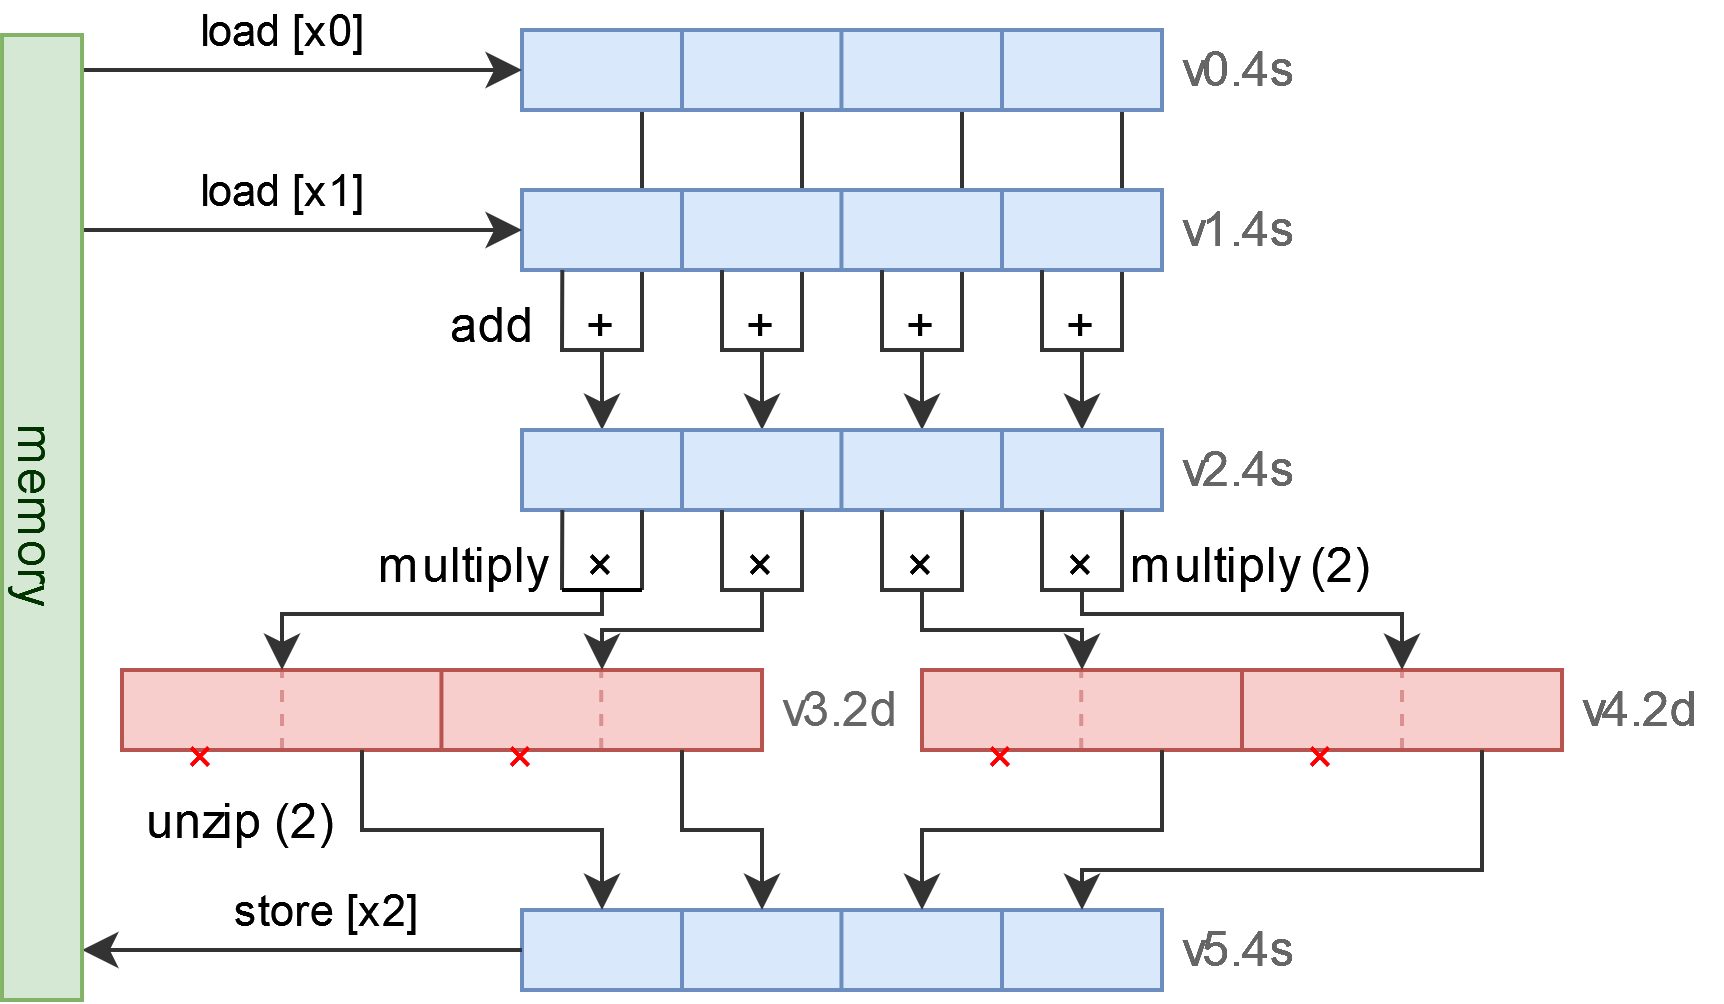
\includegraphics[width=0.8\textwidth]{neon/neon_example.drawio.png}
  \caption{Visual representation of the NEON registers and instructions in Algorithm~\ref{alg:neoninstructions}.}
  \label{fig:neonexample}
\end{figure}

\subsection{Cortex-A72 Micro-Architecture}
For profiling and benchmarking our code, we use a Raspberry Pi 4 Model B, which has a 64-bit quad-core ARM Cortex-A72 CPU that uses the \mbox{ARMv8-A} architecture (which is a specific profile of ARMv8). The term \mbox{`Cortex-A72 Micro-Architecture'} refers to the specific design of the\linebreak \mbox{ARM Cortex-A72 CPU}, which differs from other CPUs that implement the \mbox{ARMv8-A} architecture.

We work with the A64 instruction set, combined with the NEON extension. Unfortunately, the Cortex-A72 does not support the Crypto extension, which means that we cannot use hardware acceleration for cryptographic operations such as SHA-3~\cite{dworkin2015sha}.

\subsubsection{Core pipeline}
The core pipeline of the Cortex-A72 consists of 15 stages which are split into a front-end and a back-end. A high-level overview of the instruction processing pipeline~\cite{CortexA72OptGuide} is shown in Figure~\ref{fig:cortexa72pipeline}.

\begin{figure}
  \centering
  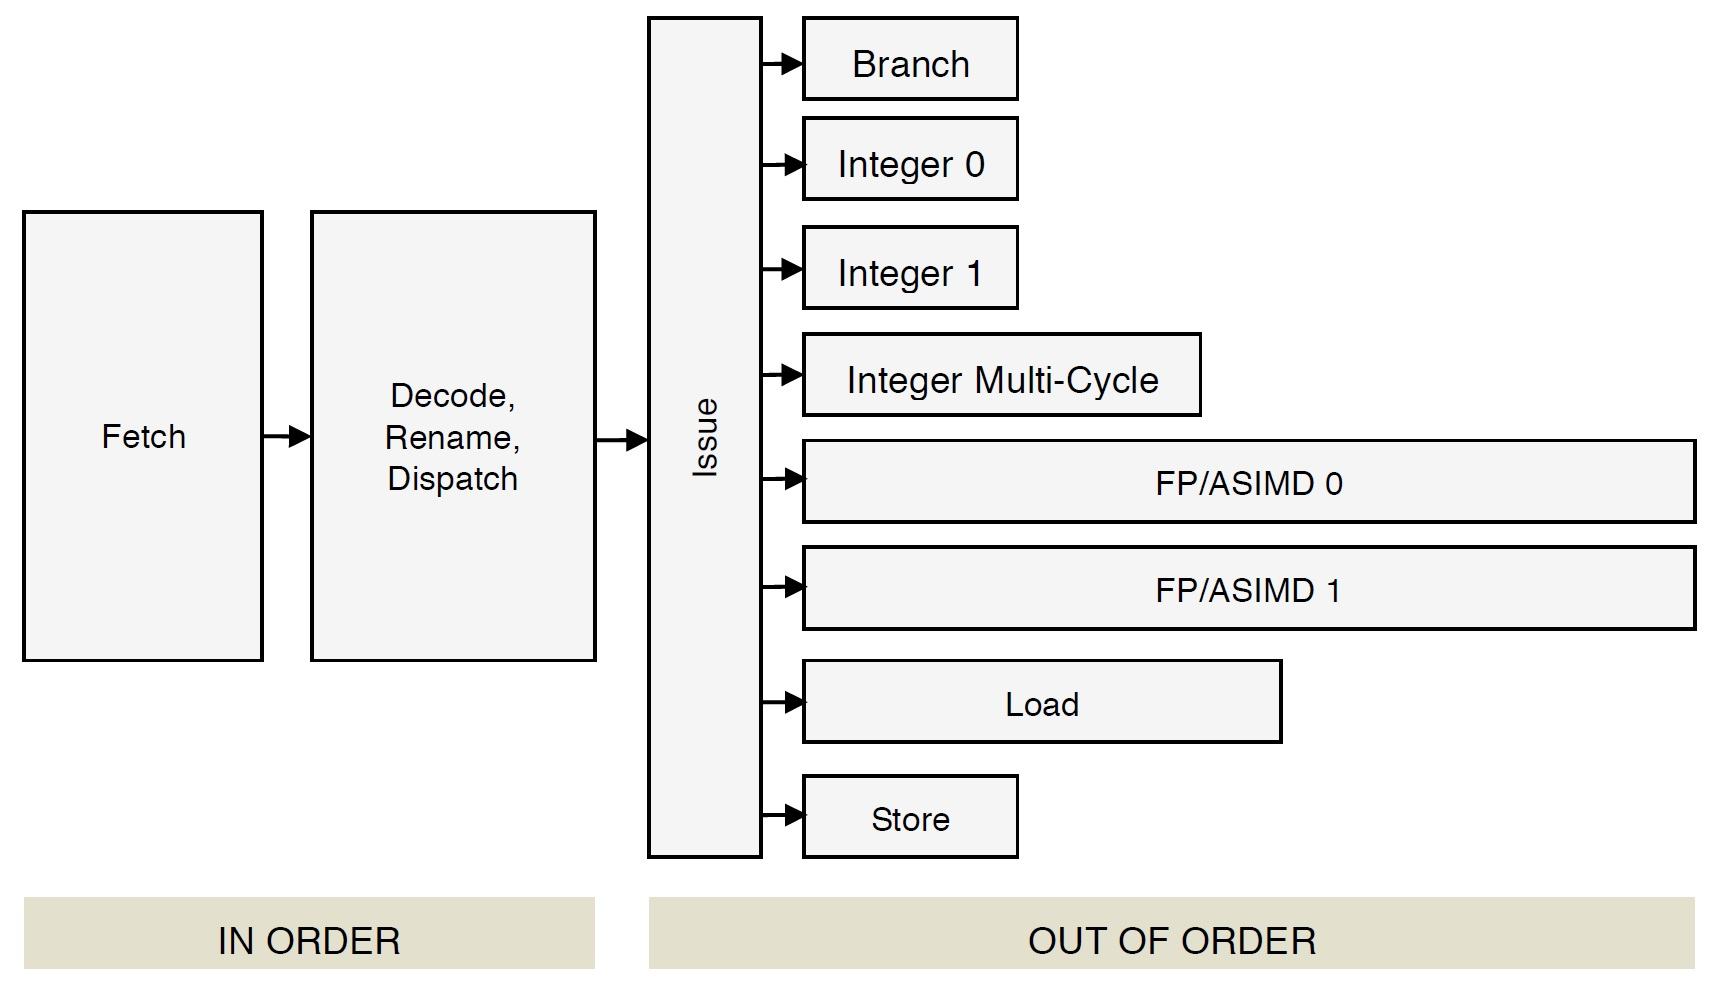
\includegraphics[width=0.8\textwidth]{armv8/Cortex-A72-pipeline-simplified.jpg}
  \caption{High-level overview of the ARM Cortex-A72 instruction processing pipeline~\cite{CortexA72OptGuide}.}
  \label{fig:cortexa72pipeline}
\end{figure}

The pipeline consists of two parts:
\begin{enumerate}
  \item \textbf{Front-end} (In Order): This part of the pipeline is responsible for fetching and decoding incoming instructions into micro-ops: smaller instructions that are easier to execute. These micro-ops are then fed into the back end. The front end works on instructions in order, meaning that it processes them in the order that they are received.
  \item \textbf{Back-end} (Out of Order): This part of the pipeline is responsible for executing the micro-ops that are generated by the front end. It consists of multiple pipelines that serve different purposes, such as branching, integer arithmetic, NEON operations, and memory operations. The back-end pipelines can execute micro-ops out of order, meaning they can execute operations in a different order than they were received.
\end{enumerate}

The front-end can work on 3 instructions at the same time and it can dispatch up to 5 micro-ops per cycle to the back-end~\cite{SandSoftwaresound2024}. The back-end pipelines can execute one or two micro-ops per cycle, depending on the specific pipeline. The main goal of the front end (and this structure in general) is to make sure that the back-end pipelines are always filled with micro-ops to minimize stalls (where a pipeline has to wait for an earlier operation to finish).

\subsubsection{Assembly instructions and latency}
In this thesis, we use A64 assembly instructions to optimize the MEDS implementation. Each used instruction has three relevant properties:
\begin{itemize}
  \item \textbf{Execution latency}: The number of CPU cycles after starting an instruction that it takes for the results of that instruction to be available for usage in the next instruction.
  \item \textbf{Execution throughput}: The maximum amount of times that a particular instruction can be executed per cycle.
  \item \textbf{Utilized pipeline}: The back-end pipeline(s) that this instruction uses.
\end{itemize}

As the Cortex-A72 uses an out-of-order execution model, it is impossible to provide instruction timing information that will predict how long a certain instruction will take to execute in a certain context~\cite{CortexA72OptGuide}. Nevertheless, the execution latency and throughput of instructions provide valuable information about the performance of that instruction. Therefore, we list the execution latency and throughput of the NEON instructions that we use in the assembly code that was written for this thesis in Table~\ref{tab:neonlatencythroughput}. We also use many intrinsic functions in the C code, which are functions that map directly to assembly instructions. However, as the compiler is still able to reorder and optimize these instructions, it is not directly beneficial to know the latencies and throughputs of these instructions.

\begin{table}
  \centering
  \caption{ARM Cortex-A72 latency and throughput for the NEON assembly instructions used in this thesis~\cite{CortexA72OptGuide}.}
  \resizebox{\textwidth}{!}{
    %
    \begin{tabular}{llrr}
      \toprule
      \textbf{Instruction} & \textbf{Description}               & \textbf{Latency} & \textbf{Throughput} \\
      \midrule
      \texttt{ld1}         & Load from memory                   & 5                & 1                   \\
      \texttt{st1}         & Store to memory                    & 5                & 1                   \\
      \midrule
      \texttt{umull}       & Unsigned multiply long             & 4                & 1                   \\
      \texttt{umull2}      & Unsigned multiply long (high half) & 4                & 1                   \\
      \texttt{umlal}       & Uns. mult. long \& accumulate      & 4                & 1                   \\
      \texttt{mls}         & Multiply subtract                  & 5                & 1/2                 \\
      \texttt{add}         & Add                                & 3                & 2                   \\
      \texttt{sub}         & Subtract                           & 3                & 2                   \\
      \texttt{and}         & Bitwise AND                        & 3                & 2                   \\
      \texttt{ushr}        & Unsigned shift right               & 3                & 1                   \\
      \midrule
      \texttt{dup}         & Store in all lanes                 & 8                & 1                   \\
      \texttt{ins}         & Store in one lane                  & 3                & 2                   \\
      \texttt{xtn}         & Extract and narrow                 & 3                & 2                   \\
      \texttt{uzp1}        & Unzip (keep low)                   & 3                & 2                   \\
      \texttt{uzp2}        & Unzip (keep high)                  & 3                & 2                   \\
      \midrule
      \texttt{cmeq}        & Compare equal                      & 3                & 2                   \\
      \texttt{cmhs}        & Compare higher or same             & 3                & 2                   \\
      \bottomrule
    \end{tabular}
    %
  }
  \label{tab:neonlatencythroughput}
\end{table}

\subsubsection{Instruction scheduling}
At first glance, it might seem that the order in which instructions of a certain instruction sequence are written in the assembly/intrinsic code influences the performance of the code, as the latencies and throughputs of the various instructions can influence the execution time of the code. This is the case for earlier ARM architectures, where hand-tuning of the instruction order could lead to performance improvements. However, the out-of-order pipeline of the Cortex-A72 can schedule and execute the instructions of a certain instruction sequence optimally without the need for hand-tuning the instruction order~\cite{ARM_Cortex_A72_TRM}. This means that the CPU can `hide' the latencies of instructions (by executing other micro-ops in the meantime) at least as well as hand-tuned code would be able to do. This is very beneficial for our work, as it means that we can focus on writing clean and readable code without having to worry about the order of the instructions.

It is important to note that this does not mean that there are no benefits to knowing the latencies and throughputs of instructions. Choosing a different sequence of instructions to compute the same result can still have an impact on the performance of the code because some instructions might be better suited for that specific computation.

\section{Optimizing cryptographic schemes}
\label{sec:optimizingcrypto}
When programming or optimizing cryptographic schemes or primitives, it is essential that the security of the scheme is not compromised because of vulnerabilities that are introduced in the code. One of the most important aspects in this context is the notion of constant-time execution~\cite{kocher1996timing}. A cryptographic function is said to be executed in constant-time if there exist no side-channel attacks that can extract secret information (such as a private key) by looking at the execution time of the function or any sub-sequence of the instructions in the function. In this section, we go over the main pitfalls that can lead to non-constant-time execution.

\subsection{Branching and conditional execution}
\label{sec:branching}
One of the most common reasons for non-constant-time execution occurs when the code contains branches that depend on secret data, allowing an attacker to perform a timing attack. A timing attack is a side-channel attack where an attacker measures the time that it takes to execute a certain piece of code and uses this measurement to derive information about the secret data that is used in the code. Consider the example in Algorithm~\ref{alg:branchingsecretdata}.

\begin{algorithm}
  \caption{Branching on secret data (unsafe)}
  \label{alg:branchingsecretdata}
  \begin{algorithmic}[1]
    \If{$\text{secret\_data} = 0$}
    \State \Call{doExpensiveOperation}{}() \Comment{This operation is slow}
    \Else
    \State \Call{doCheapOperation}{}() \Comment{This operation is fast}
    \EndIf
  \end{algorithmic}
\end{algorithm}

The execution time of this code snippet depends on the value of `secret\_data'. If `secret\_data' is 0, the execution time will be longer than when `secret\_data' is not 0, allowing an attacker to derive information about the value of `secret\_data' by measuring the execution time of the code.

Another example of branching on secret data occurs when the code uses a loop in which the execution time depends on secret data. Consider the example in Algorithm~\ref{alg:loopsecretdata}.

\begin{algorithm}
  \caption{Looping on secret data (unsafe)}
  \label{alg:loopsecretdata}
  \begin{algorithmic}[1]
    \For{$i = 0$ to $\text{secret\_data}$}
    \State \Call{doSomething}{}()
    \EndFor
  \end{algorithmic}
\end{algorithm}

Obviously, the execution time of this code snippet depends on the value of `secret\_data'.

\subsubsection{Compiler optimizations and branch prediction}
The previous examples are relatively obvious, but there are many more subtle ways in which branching on secret data can occur, especially when working with a smart compiler that tries to optimize the code. Consider the following example in Algorithm~\ref{alg:conditionalswap}.

\begin{algorithm}
  \caption{Conditional swap (unsafe)}
  \label{alg:conditionalswap}
  \begin{algorithmic}[1]
    \Function{conditionalSwap}{$x, y, \text{secret\_data}$}
    \If{$\text{secret\_data} = 1$}
    \State $x, y \gets y, x$
    \Else
    \State $x, y \gets x, y$
    \EndIf
    \State \Return $x, y$
    \EndFunction
  \end{algorithmic}
\end{algorithm}

Although it might seem that this function is safe, nearly all compilers will optimize this code such that the assignment in the `else' branch is removed, making a timing attack possible.

Even if you can guarantee that the compiler does not optimize this code, the `branch prediction' feature in modern CPUs might still make a timing attack possible. Branch prediction is a technique that tries to predict the outcome of a branch instruction before it is executed, allowing a CPU to start executing the instructions within the predicted branch. If the prediction is correct, the code will execute faster, but if the prediction is incorrect, the CPU will need to discard the results and start executing the correct branch, causing a delay. If an attacker knows how the CPU will predict the branch, they can use this information to perform a timing attack.

\subsubsection{Mitigating timing attacks}
The most important technique to mitigate timing attacks on conditional execution is to never branch on secret data at all, not even if it seems safe. Most common operations can be rewritten in a way that removes conditional execution. For example, the conditional swap operation in Algorithm~\ref{alg:conditionalswap} can be rewritten as shown in Algorithm~\ref{alg:conditionalswapfixed}.

\begin{algorithm}
  \caption{Conditional swap (safe)}
  \label{alg:conditionalswapfixed}
  \begin{algorithmic}[1]
    \Function{conditionalSwap}{$x, y, \text{secret\_data}$}
    \State $d \gets (x \oplus y) \cdot \text{secret\_data}$ \Comment{`$\oplus$' is the XOR operation}
    \State $x \gets x \oplus d$
    \State $y \gets y \oplus d$
    \EndFunction
  \end{algorithmic}
\end{algorithm}

In this code snippet, if `secret\_data' is 1, $x = x \oplus (x \oplus y) = y$. Otherwise, $x = x \oplus 0 = x$. This way, the code does not branch (on secret data) and is therefore safe from timing attacks, assuming the compiler does not optimize the code in such a way that the branch is reintroduced.

\subsection{Data-dependent memory access}
\label{sec:datadependentmemoryaccess}
Another common cause for non-constant-time execution is caused by accessing memory at an index that depends on secret data. Consider the example in Algorithm~\ref{alg:datadependentmemoryaccess}.

\begin{algorithm}
  \caption{Data-dependent memory access (unsafe)}
  \label{alg:datadependentmemoryaccess}
  \begin{algorithmic}[1]
    \State $x \gets \text{public\_array}[\text{secret\_data}]$
  \end{algorithmic}
\end{algorithm}

This code is susceptible to a `cache-timing attack'. A cache-timing attack is a side-channel attack where an attacker measures the time that it takes to access a certain memory location~\cite{bernstein2005cache, kocher1996timing}. If the data at that location is stored in the CPU cache, the access time will be faster than if the data is not (yet) in the cache. By measuring the time that it takes to access a certain memory location, an attacker can infer information about the value of `secret\_data'.

This is only the most basic form of a cache-timing attack. More advanced attacks can be performed if the attacker has more control over the system, such as the ability to manipulate the cache to ensure that the data is (or is not) in the cache. Although there exist techniques to mitigate these attacks (such as always accessing every index of the array), it is best to avoid accessing memory at an index that depends on secret data altogether.

\subsection{Non-constant-time operations}
\label{sec:nonconstanttimeoperations}
A final common cause for non-constant-time execution is the use of CPU instructions that do not execute in constant time. Common examples of such instructions are (integer) division, math functions such as sin/cos, and various other instructions, depending on the CPU architecture. Instructions like these can take a variable amount of time to execute, depending on the input data. It is important to avoid using such instructions with secret data.

\subsection{Preventing timing attacks with Valgrind and Timecop}
\label{sec:valgrindtimecop}
It has been shown that even if you write code that should theoretically compile to a constant-time binary, the compiler might still optimize the code in such a way that it is vulnerable to various kinds of timing attacks~\cite{barthe2019formal, simon2018you}. Therefore, it is good practice to make sure the resulting binary is indeed constant-time.

Vulnerabilities to timing attacks described in Section~\ref{sec:branching} and Section~\ref{sec:datadependentmemoryaccess} can be detected using Valgrind~\cite{nethercote2007valgrind} using a technique that was described by Langley~\cite{langley2010checking}. Valgrind is a programming tool that is used to detect memory leaks, buffer overflows, and other memory-related problems. Among many other things, Valgrind can detect branching on uninitialized data and memory accessing at an uninitialized index. Valgrind is unable to detect timing attack vulnerabilities caused by non-constant-time operations such as mentioned in Section~\ref{sec:nonconstanttimeoperations}. Using the following routine, we can use Valgrind to detect timing attack vulnerabilities:
\begin{enumerate}
  \item \textbf{Uninitialized secret data}: Make sure our code does not initialize any secret data. Normal operations (such as arithmetic operations) on uninitialized data are ignored by Valgrind.
  \item \textbf{Run Valgrind}: Run Valgrind on our code. Any resulting complaints about uninitialized data are possible locations at which a vulnerability to a timing attack might exist.
\end{enumerate}

Timecop~\cite{timecop} provides a \texttt{poison.h} header file that can be used to poison secret data, which essentially makes it uninitialized. This can be used in combination with Valgrind to detect timing attack vulnerabilities.

\section{Modular reduction}
\label{sec:preliminariesmodularreduction}
As MEDS is a cryptographic scheme that operates on elements in a finite field, modular reduction is a basic building block that is used in many parts of the scheme. Various algorithms can be used to perform modular reduction. In this section, we go over the most common algorithms.

\begin{itemize}
  \item \textbf{Naive reduction}\\
        The naive reduction algorithm is slow and not suitable for our purposes, but we use it as a baseline to compare the other algorithms to. This algorithm works by applying an integer division instruction to the input, followed by a multiplication with the modulus and a subtraction. A big disadvantage of this approach is that division is not a constant time operation, which can lead to timing attacks (see Section~\ref{sec:nonconstanttimeoperations}). Furthermore, the division operation is usually relatively slow compared to other operations.
  \item \textbf{Montgomery reduction}\\
        Montgomery reduction~\cite{montgomery1985modular} is a modular reduction algorithm that is based on the Montgomery multiplication algorithm. It does not use a division instruction, which makes it suitable for constant time operations. Instead, it works by subtracting a multiple of the modulus from the input such that the input is (almost) smaller than the modulus. The algorithm requires the input and outputs to be converted to and from a Montgomery representation.
  \item \textbf{Barrett reduction}\\
        Barrett reduction~\cite{barrett1986implementing} is a modular reduction algorithm that is similar to Montgomery reduction in the sense that it also subtracts a multiple of the modulus from the input. However, it does not require the input to be converted to a different representation. Additionally, the cost of the reduction is slightly lower for small inputs compared to Montgomery reduction.
\end{itemize}

Montgomery reduction is generally very efficient when a large chain of multiplications is required and the overhead of converting to and from Montgomery representation is negligible compared to the number of multiplications/reductions, whereas Barrett reduction is typically a bit faster for small inputs.

\subsection{Barrett reduction}
\label{sec:barrettreduction}
Barrett reduction works by approximating the modular reduction. Given an unsigned integer $a$ and a modulus $n$,
\[
  a \bmod n = a - \left\lfloor \frac{a}{n} \right\rfloor \cdot n.
\]

From this, the Barrett reduction formula for unsigned integers can be derived (Definition~\ref{def:barrettreduction}).

\begin{definition}[Barrett reduction for unsigned integers]~\\
  \label{def:barrettreduction}
  Let $a$ be an unsigned integer and $n$ be a modulus.
  Let $R$ be a constant such that $R = 2^k > n$ for some $k$. Then:
  \[
    a \bmod n = a - \left\lfloor \frac{a \cdot \left[\frac{R}{n}\right]}{R} \right\rfloor \cdot n.
  \]
  where $\left[\frac{R}{n}\right]$ represents $\frac{R}{n}$ rounded up or down, depending on the choice of the rounding operation.
\end{definition}

As $R$ is a power of 2, the division by $R$ can be implemented as a cheap right-shift operation. Additionally, the value of $m = \left[\frac{R}{n}\right]$ can be precomputed because the modulus $n$ is a constant. This leaves us with two things to choose: the value of $k$ and the rounding operation.

\subsubsection{Choice of $k$}
\label{sec:choiceofk}
Usually, the value of $k$ chosen for Barrett reduction is as small as possible such that $2^k > n$. Combined with setting the rounding function of the precomputed value to the `floor' function, this results in a reduction that reduces to a value between $0$ and $2n-1$, requiring an additional conditional subtraction at the end of the reduction. Choosing a larger value of $k$ has one major disadvantage: the precomputed value $m = \left[\frac{R}{n}\right]$ becomes larger, which means that the multiplication $a \cdot m$ will result in a larger value (possibly leading to a register overflow). However, choosing a larger value of $k$ can also be beneficial: the quotient $m$ will be closer to the actual value of $\frac{R}{n}$, which means that the reduction will be more accurate. If we know that the input $a$ will never be larger than a particular value, we can choose $k$ such that the conditional subtraction at the end of the reduction is not required. For this to work, we need to use the ceiling function for the rounding operation.

\chapter{Profiling}
\label{ch:profiling}
In this chapter, we discuss and execute the profiling of the optimized MEDS implementation from~\cite{chou2024reducing}, with the goal of identifying the code sections that take up the most time. We use this information to optimize the code in the next chapter.

\section{Profiling techniques}
To obtain a better understanding of the performance of (specific functions of) MEDS, we need to profile the implementation. Profiling is the process of measuring the space or time complexity of a program or a specific function. The goal of profiling is to identify the bottlenecks in the speed or memory usage of a program: these are the parts of the program that take the most time or memory. Usually, we hope that a small part of the program is responsible for a large part of the time or memory usage and that this part can be optimized to improve the overall performance.

Typically, profiling is done by running the program with a profiler. There exist a wide variety of profilers for C, such as GProf~\cite{graham1982gprof}, Valgrind~\cite{nethercote2007valgrind}, and Linux-Perf~\cite{de2010new}. In our case, the most accurate way to measure the performance is to measure the number of cycles that are used by the program or a specific function, which can be done with Linux-Perf.

\subsection{Cycle counting}
Cycle counting is a technique that is used to measure the number of CPU cycles that it takes to execute a certain program or function. This is usually done by accessing the performance monitoring unit (PMU) of the CPU, which is a CPU component that measures the performance of the processor. Typically, these PMUs contain a register that can be read to obtain the number of cycles executed since a certain point in time. On Linux, we can access this data using the Linux-Perf tool~\cite{de2010new}, which can be used to measure the number of instructions executed, the number of cache misses, etc.

\subsubsection{Advantages}
The advantages of profiling the code using a cycle counter are:
\begin{itemize}
  \item \textbf{Accurate}: Measuring the cycle counter results in the most accurate measurement of time. For comparison, using a technique that measures the current time in (nano)seconds is less accurate, because the CPU is capable of executing multiple cycles in a single nanosecond.
  \item \textbf{Low overhead}: Measuring the cycle counter has a very low additional performance overhead to the program, as it usually consists of reading a single register.
  \item \textbf{Precise}: By annotating the code with our own cycle counter, we can measure the performance of specific functions or even specific lines of code.
\end{itemize}

\subsubsection{Disadvantages}
The disadvantages of profiling the code using a cycle counter are:
\begin{itemize}
  \item \textbf{Interference}: The program to be measured shares the CPU (core) with other programs, which can interfere with measurements. If another program is switched in by the operating system, the cycle counter will also count the cycles that were used by this program. Although this usually does not have a big impact on profiling results, this can be problematic for obtaining accurate benchmarks.
  \item \textbf{Architecture}: The way in which the cycle counter is accessed is different for each architecture. However, since we use the Linux-Perf tool, this is abstracted away for us.
\end{itemize}

\subsubsection{Problem mitigation}
There are a few problems with cycle counting that we need to mitigate. First of all, there are some features on modern CPUs that will cause cycle counting to produce inaccurate results. These features include frequency scaling (based on the current workload, a CPU can change its clock frequency to save power) and hyperthreading (multiple threads share the same CPU core at the same time by interleaving instructions). It is essential to disable these features to obtain accurate results.

\pagebreak

Another problem is program interference (see above). Unfortunately, this is a problem that is hard to prevent completely, but we can work around it. By running the program multiple times and taking the median of the results, we can reduce the impact of interference on the results. This is a common technique in benchmarking and is used in many other cryptographic papers~\cite{becker2021neon,ducas2018crystals}.

\section{MEDS profiling results}
\label{sec:medsprofilingresults}

\subsection{Measurement setup}
We added cycle count measurements to all MEDS functions that we anticipate will require a significant amount of time. We decided to profile the code for the MEDS-55520 parameter set, which is in the middle of the three parameter sets in terms of security level. The results are representative of the other parameter sets as well, only the scale is different. We executed measurements for the three algorithms of a digital signature scheme: key generation, signing, and verification. The results are shown in Tables~\ref{tab:medskeygenfunctions} (key generation),~\ref{tab:medssigningfunctions} (signing), and~\ref{tab:medsverificationfunctions} (verification). For each algorithm, we list the functions or code sections that take up more than 1\% of the total number of cycles. We provide the number of megacycles (MCycles) that were used in that function, the percentage of the total number of cycles that were used by that function, and the number of times that function was called. Note that the number of cycles cannot be divided by the number of calls to obtain the average number of cycles per call, because the number of cycles that are used by a function can depend on the input.

\begin{table}
  \centering
  \caption{MEDS-55520 key generation profiling results.}
  \begin{tabular}{lrrr}
    \toprule
    \textbf{Function}        & \textbf{\# MCycles} ($\pm$) & \textbf{\% of Total} ($\pm$) & \textbf{\# Calls} \\
    \midrule
    \texttt{pmod\_mat\_mul}  & 15.98                       & 69.78                        & 70                \\
    \texttt{pmod\_mat\_syst} & 2.08                        & 9.07                         & 6                 \\
    \texttt{rnd\_sys\_mat}   & 2.07                        & 9.05                         & 1                 \\
    \texttt{solve\_opt}      & 1.42                        & 6.20                         & 1                 \\
    \texttt{bs\_fill}        & 1.06                        & 4.63                         & 1                 \\
    \midrule
    Cumulative               & 22.61                       & 98.73                        &                   \\
    Remaining                & 0.29                        & 1.27                         &                   \\
    \bottomrule
  \end{tabular}
  \label{tab:medskeygenfunctions}
\end{table}

\begin{table}
  \centering
  \caption{MEDS-55520 signing profiling results.}
  \begin{tabular}{lrrr}
    \toprule
    \textbf{Function}         & \textbf{\# MCycles} ($\pm$) & \textbf{\% of Total} ($\pm$) & \textbf{\# Calls} \\
    \midrule
    \texttt{pmod\_mat\_mul}   & 2518.85                     & 69.17                        & 14635             \\
    \texttt{pmod\_mat\_syst}  & 391.36                      & 10.75                        & 1040              \\
    \texttt{solve\_opt}       & 293.44                      & 8.06                         & 208               \\
    \texttt{bs\_fill}         & 212.74                      & 5.84                         & 1                 \\
    \texttt{shake256\_absorb} & 203.06                      & 5.58                         & 212               \\
    \midrule
    Cumulative                & 3619.46                     & 99.39                        &                   \\
    Remaining                 & 22.24                       & 0.61                         &                   \\
    \bottomrule
  \end{tabular}
  \label{tab:medssigningfunctions}
\end{table}

\begin{table}
  \centering
  \caption{MEDS-55520 Verification profiling results.}
  \begin{tabular}{lrrr}
    \toprule
    \textbf{Function}         & \textbf{\# MCycles} ($\pm$) & \textbf{\% of Total} ($\pm$) & \textbf{\# Calls} \\
    \midrule
    \texttt{pmod\_mat\_mul}   & 2537.20                     & 69.24                        & 14560             \\
    \texttt{pmod\_mat\_syst}  & 393.22                      & 10.73                        & 1040              \\
    \texttt{solve\_opt}       & 294.20                      & 8.03                         & 208               \\
    \texttt{bs\_fill}         & 212.88                      & 5.81                         & 1                 \\
    \texttt{shake256\_absorb} & 203.31                      & 5.55                         & 267               \\
    \midrule
    Cumulative                & 3640.80                     & 99.35                        &                   \\
    Remaining                 & 23.80                       & 0.65                         &                   \\
    \bottomrule
  \end{tabular}
  \label{tab:medsverificationfunctions}
\end{table}

% \begin{tikzpicture}
%   \pie[
%     sum=100,
%     text=legend,
%     % pos={8,0},
%     % explode=0.1,
%     color={pie3,pie4,pie5,pie6,pie7,pie8,pie9}
%   ]{59.3/matmul, 17.1/matsyst, 6.1/shakeabsorb, 1.2/GFinv, 16.3/Other}
%   \pie[
%     sum=100,
%     color={pie3,pie4,pie5,pie6,pie7,pie8,pie9},
%     hide number
%   ]{59.3/,17.1/,6.1/,1.2/1.2\%}
%   \pie[
%     sum=100,
%     color={pie3,pie4,pie5,pie6,pie7,pie8,pie9}
%   ]{59.3/,17.1/,6.1/}
% \end{tikzpicture}

\subsection{Result analysis}
Because of the way that MEDS works, the results of the signing and verification operations are very similar. For key generation, the results in the table account for 98.76\% of the total number of cycles. For signing and verification, this number is 99.42\% and 99.39\%, respectively. In all three algorithms, the remainder of the cycles is spent on a large set of functions that take up a small amount of time. Given that there are only a few functions that take up a significant amount of time, we can conclude that the performance of MEDS is mostly determined by these functions.

\subsubsection{Matrix multiplication}
For all three operations, the \texttt{pmod\_mat\_mul} function takes up the most time, almost 70\%. This function is used to multiply two matrices $A \in \mathbb{F}_q^{m \times n}$ and $B \in \mathbb{F}_q^{n \times o}$ over a finite field $\mathbb{F}_q$. The function is implemented in MEDS using a naive algorithm that computes the dot product of each row of $A$ with each column of $B$, followed by a reduction modulo $q$. As will be shown in Section~\ref{sec:matrixmultiplicationcomplexity}, the time complexity of this algorithm is $\mathcal{O}(mno)$ ($= \mathcal{O}(n^3)$ for square matrices).
% This is so much time that I was not able to finish this thesis. Mic drop; I am a failure. <- van fringerlie

\subsubsection{Matrix systemizer}
The \texttt{pmod\_mat\_syst} function (\texttt{pmod\_mat\_syst\_ct\_partial\_swap\_backsub} in the code, but shortened for readability) is responsible for about 11\% of the total number of cycles for signing and verification. This function is used to systemize a matrix $A \in \mathbb{F}_q^{m \times n}$ over a finite field $\mathbb{F}_q$ (see Section~\ref{sec:systemizer}). This is done using a Gaussian elimination algorithm that has a complexity of $\mathcal{O}(m^2n)$ (this is calculated in Section~\ref{sec:matrixsystemizercomplexity}).

\subsubsection{Isometry derivation}
The \texttt{solve\_opt} function is responsible for about 8\% of the total number of cycles for signing and verification. This function derives an isometry mapping $\phi = (\textbf{A} \in \mathbb{F}_q^{m \times m}, \textbf{B} \in \mathbb{F}_q^{n \times n})$ by constructing and solving a sparse system of linear equations, see Section~\ref{sec:derivingisometry}. The algorithm has a complexity of $\mathcal{O}(n^3)$.

\subsubsection{Bitstream filling}
The \texttt{bs\_fill} section is responsible for about 6\% of the total number of cycles for signing and verification. In this section of the code, multiple calls are made to the \texttt{bs\_init}, \texttt{bs\_write}, and \texttt{bs\_finalize}. We decided to group them because they are all part of the same operation: filling a bitstream with elements of the finite field $\mathbb{F}_q$. In the MEDS parameter sets that we consider, the finite field is $\mathbb{F}_{4093}$, which means that the bitstream is filled with 12-bit elements. This is done to reduce the number of bytes required to store a list of field elements.

\subsubsection{SHAKE256}
\label{sec:shake256}
A small percentage of the total number of cycles in each of the three operations is used by either \texttt{shake256\_squeeze} or \texttt{shake256\_absorb}. SHAKE256 is an extendable output function (XOF). It is part of the SHA-3 family~\cite{dworkin2015sha} and is based on the KECCAK sponge construction~\cite{bertoni2013keccak}. MEDS uses SHAKE256 to generate random field elements and to hash the challenge strings that are used in the Fiat-Shamir transform (see Section~\ref{sec:medsworks}).

\subsubsection{Random systemized matrix generation}
The \texttt{rnd\_sys\_mat} function is responsible for about 9\% of the total number of cycles for key generation. This function is used to generate a random systemized matrix over a finite field $\mathbb{F}_q$. Nearly all of its cycles are spent on generating random field elements using the \texttt{shake256\_squeeze} function (see above).

\chapter{Methodology}
\label{ch:methodology}
We have established two approaches to optimize the MEDS implementation. These approaches are not specific to ARMv8, but their implementation will be tailored to the ARMv8 architecture. Note that the two approaches are mutually exclusive, meaning they cannot be combined. We implement both approaches and evaluate their performance to determine which approach gives the highest speedup.
\begin{itemize}
  \item \textbf{Low-level optimization}:\\
        This approach focuses on optimizing the MEDS implementation at a low level. This means that we look at individual functions (such as matrix multiplication and the matrix systemizer) that take up a significant amount of time and optimize them. The input and output of these functions are thus not changed, but the way in which the result is computed is optimized using techniques such as vectorization.
  \item \textbf{High-level optimization}:\\
        This approach focuses on optimizing the MEDS implementation at a high level. The Fiat-Shamir transform used in MEDS (see Section~\ref{sec:fiatshamir}) uses $t$ challenges, where $t$ is a parameter set according to the target security level. The values of $t$ for each parameter set are displayed in Table~\ref{tab:medsparametersets} (Section~\ref{sec:parametersets}). As can be seen from the algorithmic overviews in Section~\ref{sec:medsalgorithms}, the computation of each challenge (and commitment for that challenge) is done in the same way. This means that we can compute multiple commitments in parallel, which can greatly increase the performance of the scheme. As opposed to low-level optimization, this approach changes the input and output of the underlying functions to take in and return the inputs and outputs of multiple commitments at once.
\end{itemize}

\pagebreak

In this chapter, we start by discussing how we implement modular reduction, an operation that is the same for both approaches, in Section~\ref{sec:modularreduction}. We then discuss the implementation of the two approaches in Sections~\ref{sec:lowleveloptimization} and~\ref{sec:highleveloptimization}. After this, we discuss bitstream filling and the usage of an alternative hash structure (two optimizations that can be applied to both the low-level and high-level approaches) in Section~\ref{sec:bitstreamfilling} and Section~\ref{sec:hashfunctionoptimization}, respectively. Finally, we discuss a few non-constant-time optimizations that can be applied to the verification algorithm in Section~\ref{sec:nonconstanttime}.

\section{Modular reduction}
\label{sec:modularreduction}
Throughout the entirety of the MEDS implementation, modular reduction is used extensively to reduce the size of the elements modulo $q$, where $q$ is the modulus of the finite field $\mathbb{F}_q$. The finite field that is used in MEDS for the parameter sets that we consider is $\mathbb{F}_{4093}$, which means that all elements are reduced modulo 4093. In the reference implementation of MEDS, all modulo operations are done using the \texttt{\%} operator in C. As we use NEON assembly instructions and C intrinsics to optimize the MEDS implementation, we cannot rely on this operator, as it is not defined for NEON registers and there is no single-instruction alternative in assembly.

Because of this, we need to implement our own modular reduction function that can be used with NEON registers. This function must be as fast as possible, as it is used in many places in the MEDS implementation. The various modular reduction algorithms are considered in Section~\ref{sec:preliminariesmodularreduction}. Our NEON assembly implementation of both the Barrett and Montgomery reduction algorithms is shown in Algorithm~\ref{alg:neonbarretmontgomeryasm}. As can be seen from the implementation, both algorithms use the same number of instructions. We therefore choose to use Barrett reduction, as it does not require the input and output to be converted to a different representation. We further elaborate on the Barrett reduction algorithm in the remainder of this section. As we will not use the Montgomery reduction algorithm, we only add it for the sake of comparison and do not further explain how it works.

\begin{algorithm}
  \caption{NEON Barrett and Montgomery reduction for MEDS}
  \label{alg:neonbarretmontgomeryasm}
  \textbf{Input:} $a_i \in [0, 2^{29.5})$ for $0 \leq i < 4$ (in \texttt{v0.4s})\\
  \hphantom\quad\quad\quad~~$\texttt{MEDS\_p} = 4093$ (in \texttt{v2.4s})\\
  \textbf{Output:} $a_i \bmod 4093$ for $0 \leq i < 4$ (in \texttt{v0.4s})

  \begin{minipage}[t]{0.48\textwidth}
    \textbf{Barrett}\\
    $m = 0\text{x}80180481$ (in \texttt{v1.4s})\\
    \lstinputlisting[language={[x86masm]Assembler}, style=ASMStyle]{code/barrett_reduce_small_asm.s}
  \end{minipage}
  \hfill
  \begin{minipage}[t]{0.48\textwidth}
    \textbf{Montgomery}\\
    $N' = 2731$ (in \texttt{v1.4s})\\
    $R_\text{mask} = \texttt{0xFFF}$ (in \texttt{v3.4s})
    \lstinputlisting[language={[x86masm]Assembler}, style=ASMStyle]{code/montgomery_reduce_small_asm.s}
  \end{minipage}
\end{algorithm}


\subsection{Choosing \texorpdfstring{$k$}{k} for Barrett reduction}
As mentioned in Section~\ref{sec:choiceofk}, the choice of $k$ for Barrett reduction is important. If possible, we should pick a $k$ such that the reduction will not require a final conditional subtraction. Although it is possible to continue working with small values that are congruent to the original value modulo $q$ and thereby avoid the conditional subtraction, this will eventually still require a few extra instructions to make sure the final value is reduced modulo $q$. If we can find a $k$ such that the reduction will not require a conditional subtraction whilst also not requiring additional instructions, we should pick this value.

For the MEDS parameter sets that we consider, we know that all field elements fit into 12 bits. This means that any multiplication of two field elements will result in a value that fits into 24 bits. The largest possible value that any value can become (before reduction) results from the matrix multiplication algorithm, see Section~\ref{sec:matrixmultiplication}. In this algorithm, the temporary value can (for parameter set MEDS-122000) become as large as $\log_2(k \cdot (q-1) \cdot (q-1)) = \log_2(44 \cdot 4092 \cdot 4092) \approx 29.5$ bits (see Section~\ref{sec:matrixmultiplicationoptimization}). This means that we should find a $k$ such that for all $0 \leq a < 2^{30}$, the reduction will not require a conditional subtraction.

As $2^{30}$ is a relatively small number, we use a brute force approach to find the smallest $k$ that satisfies this condition. This value turns out to be $k = 43$, which gives $m = \lceil \frac{2^{43}}{4093} \rceil = 0\text{x}80180481$. This number fits nicely into 32 bits, which means that we can store it in 32-bit NEON lanes. Because of this, using $k=43$ does not require any additional instructions compared to using a smaller value of $k$.

\subsection{Implementation}
The reference code for our Barrett reduction algorithm is shown in Algorithm~\ref{alg:barrettreduction}. This algorithm does not operate on vectorized data and serves as a baseline for implementing the NEON version.

\begin{algorithm}
  \caption{MEDS Barrett reduction}
  \label{alg:barrettreduction}
  \begin{algorithmic}[1]
    \Function{reduce}{$a$}
    \State $m \gets 0\text{x}80180481$
    \State $v \gets a \cdot m$
    \State $v \gets v \gg 43$
    \State \Return $a - v \cdot 4093$
    \EndFunction
  \end{algorithmic}
\end{algorithm}

The NEON version of the Barrett reduction algorithm is shown in Algorithm~\ref{alg:neonbarretreductionc} (C code) and Algorithm~\ref{alg:neonbarretreductionasm} (assembly code). The C code uses NEON intrinsics to perform the reduction on 128-bit NEON registers. The assembly code is a direct translation of the C code to ARMv8 assembly. Both algorithms assume that the input consists of four 32-bit unsigned integers that are stored in four lanes of a 128-bit NEON register. The output can either be stored in four 32-bit lanes or four 16-bit lanes, depending on the requirements of the calling function.

\begin{algorithm}
  \caption{NEON Barrett reduction (C)}
  \label{alg:neonbarretreductionc}
  \lstinputlisting[language=C, style=CStyle]{code/barrett_reduce_c.c}
\end{algorithm}

\begin{algorithm}
  \caption{NEON Barrett reduction (assembly)}
  \label{alg:neonbarretreductionasm}
  \textbf{Input:}
  $a_i \in [0, 2^{29.5})$ for $0 \leq i < 4$ (in \texttt{v0.4s})\\
  \hphantom\quad\quad\quad~~$m = 0\text{x}80180481$ (in \texttt{v1.4s})\\
  \hphantom\quad\quad\quad~~$\texttt{MEDS\_p} = 4093$ (in \texttt{v2.4s})\\
  \textbf{Output}: $a_i \bmod \texttt{MEDS\_p}$ for $0 \leq i < 4$ (in \texttt{v0.4s})
  \lstinputlisting[language={[x86masm]Assembler}, style=ASMStyle]{code/barrett_reduce_asm.s}
\end{algorithm}

From the assembly code, we can see that the reduction is done using five instructions (not counting the optional shrink).

\subsection{Freeze operation}
A useful operation when working with numbers outside of the finite field is the `freeze' operation. This operation takes a number $a \in [0, 2n-1]$ and returns $a \bmod n$, useful after the addition of two field elements. The advantage over the reduction functions mentioned before is that this operation can be executed with fewer instructions. Additionally, the operation can be executed over eight lanes of a 128-bit NEON register (as opposed to four lanes for the reduction operation). The freeze operation is useful after (for example) two field elements are added together and need to be reduced, in which case we can do a cheaper reduction operation. The freeze operation for MEDS is shown in Algorithm~\ref{alg:freezeoperation}.

\begin{algorithm}
  \caption{MEDS Freeze Operation}
  \label{alg:freezeoperation}
  \begin{algorithmic}[1]
    \Function{freeze}{$a$}
    \If {$a \geq 4093$}
    \State $a = a - 4093$
    \EndIf
    \State \Return $a$
    \EndFunction
  \end{algorithmic}
\end{algorithm}

As explained in Section~\ref{sec:branching}, we cannot use branching in constant-time code. However, using NEON intrinsics (or assembly instructions), we can implement the freeze operation in constant time. The NEON version of the freeze operation is shown in Algorithm~\ref{alg:neonfreezeoperationc} (C code) and Algorithm~\ref{alg:neonfreezeoperationasm} (assembly code).

\begin{algorithm}
  \caption{NEON freeze operation (C)}
  \label{alg:neonfreezeoperationc}
  \lstinputlisting[language=C, style=CStyle]{code/freeze_c.c}
\end{algorithm}

\begin{algorithm}
  \caption{NEON freeze operation (assembly)}
  \textbf{Input:} $a_i \in [0, 2 \cdot 4093 - 1]$ for $0 \leq i < 4$ (in \texttt{v0.4s})\\
  \hphantom\quad\quad\quad~~$\texttt{MEDS\_p} = 4093$ (in \texttt{v1.4s})\\
  \textbf{Output}: $a_i \bmod \texttt{MEDS\_p}$ for $0 \leq i < 4$ (in \texttt{v0.4s})
  \label{alg:neonfreezeoperationasm}
  \lstinputlisting[language={[x86masm]Assembler}, style=ASMStyle]{code/freeze_asm.s}
\end{algorithm}

\section{Low-level optimization}
\label{sec:lowleveloptimization}
The low-level optimization approach focuses on optimizing the individual functions that take up a significant amount of time in the MEDS implementation. As can be seen from the profiling results displayed in Section~\ref{sec:medsprofilingresults}, over 99\% of the total number of cycles used in signing and verification is used on just five functions. In this section, we discuss the optimization of three of these functions: matrix multiplication (Section~\ref{sec:matrixmultiplication}), matrix systemizer (Section~\ref{sec:matrixsystemizer}), and isometry derivation (Section~\ref{sec:isometryderivation}). The optimization of the other two functions is not specific to the low-level optimization approach and will be discussed in Section~\ref{sec:bitstreamfilling} (bitstream filling) and Section~\ref{sec:hashfunctionoptimization} (SHAKE256).

\subsection{Matrix multiplication}
\label{sec:matrixmultiplication}
Matrix multiplication is by far the most time-consuming function in MEDS, taking up almost 70\% of the total number of cycles in key generation, signing, and verification. The function is responsible for the simple task of multiplying two matrices $A \in \mathbb{F}_{4093}^{m \times n}$ and $B \in \mathbb{F}_{4093}^{n \times o}$ over the finite field $\mathbb{F}_{4093}$.

\subsubsection{Complexity analysis}
\label{sec:matrixmultiplicationcomplexity}
Matrix multiplication is implemented using a naive algorithm (see Algorithm~\ref{alg:medsmatrixmultiplication} in Appendix~\ref{app:supplementalalgs}) that works by calculating the dot product of each row of $A$ with each column of $B$, followed by a reduction modulo 4093. Three nested loops loop over the $m$ rows of $A$, the $o$ columns of $B$, and the $n$ columns of $A$ and rows of $B$. The resulting time complexity of this algorithm is therefore $\mathcal{O}(mno)$. Algorithms have been developed that can multiply two matrices in a lower time complexity, such as the Strassen algorithm~\cite{strassen1969gaussian} and (generalizations of) the Coppersmith-Winograd algorithm~\cite{coppersmith1987matrix}. However, these algorithms have such a high constant factor that they are not suitable for our purposes. Instead, we focus on optimizing the naive algorithm.

\subsubsection{Optimization}
\label{sec:matrixmultiplicationoptimization}
We optimize matrix multiplication by applying vectorization to the naive algorithm. We compute the dot product of multiple rows of $A$ with multiple columns of $B$ at the same time.

Our first observation lies in the fact that all intermediate values that are computed while calculating the dot product fit into 32 bits.
\begin{itemize}
  \item Given $A \in \mathbb{F}_q^{m \times n} \times B \in \mathbb{F}_q^{n \times o} = C \in \mathbb{F}_q^{m \times o}$, the maximum value of $n$ for all matrix multiplications in all MEDS parameter sets is 44 (MEDS-122000).
  \item The values stored in $A$ and $B$ are field elements that fit into 12 bits. Their value is 4092 at most.
  \item In the computation of a single element of $C$, exactly $n$ multiplications are performed, which are all added together.
  \item This means that $n$ values are added together, which results in a value that fits in $\log_2(n \cdot 4092 \cdot 4092) = \log_2(44 \cdot 4092 \cdot 4092) \approx 29.5$ bits.
\end{itemize}
As a result, we do not need to reduce the intermediate values modulo 4093 during the computation of the dot product if we accumulate the multiplications of the 16-bit values into 32-bit registers. Instead, we can reduce the resulting value after the dot product is computed. From this observation, we can derive that we can compute the dot product of four rows of $A$ with four columns of $B$ at the same time, as we can fit four 32-bit values in four lanes of a 128-bit NEON register.

However, we can do slightly better than that. The NEON unit is capable of performing four (widening) multiplications of 16-bit unsigned integers at the same time, but a NEON register can hold eight 16-bit unsigned integers. This means that we can compute the dot product of eight rows of $A$ with eight columns of $B$ using two multiplication instructions. This does not change the total number of multiplications that need to be performed, but it does halve the number of memory loads and stores that need to be executed.

Unfortunately, we cannot directly apply an easy 8-way vectorization to (one of) the loops in the naive algorithm. The NEON unit can load 128 bits of data from memory at a time, but it is not able to do this with an arbitrary distance between the elements. The matrices in MEDS are stored in row-major order (each row is stored after the previous row), meaning we can load eight elements of a row using a single NEON instruction, but we cannot load eight elements of a column using a single NEON instruction. An easy solution would be to transpose matrix $B$ before performing the multiplication, but this would require additional memory and time to perform the transpose.

Instead, we use an approach where 16 dot products are computed at the same time, in the form of an $8\times8$ submatrix of $C$. We load an $8\times8$ submatrix of $A$ and an $8\times8$ submatrix of $B$ into NEON registers and compute the dot product of these submatrices, adding the result to the submatrix of $C$. We repeat this process until all dot products are computed and stored in $C$. The resulting algorithm is shown in Algorithm~\ref{alg:vectorizedmatrixmultiplication}. A visualization of the functionality of this algorithm is shown in Figure~\ref{fig:vectorizedmatrixmultiplication}. This algorithm works for matrices of which the dimensions are multiples of eight.

\begin{algorithm}
  \caption{Vectorized matrix multiplication for matrices that are multiples of eight in size}
  \label{alg:vectorizedmatrixmultiplication}
  \begin{algorithmic}[1]
    \Function{matrix\_mul}{$A \in \mathbb{F}_q^{m \times n}, B \in \mathbb{F}_q^{n \times o}$}
    \State $C \gets \text{zero matrix of size } m \times o$
    \For{$c \gets 0$ to $m$ in steps of 8}
    \For{$r \gets 0$ to $o$ in steps of 8}
    \State $C_0, \dots, C_7 \gets \text{empty NEON register}$
    \For{$k \gets 0$ to $n$ in steps of 8}
    \State $A_0, \dots, A_7 \gets \text{load } 8\times8 \text{ submatrix at } A[r][k]$
    \State $B_0, \dots, B_7 \gets \text{load } 8\times8 \text{ submatrix at } B[k][c]$
    \For{$i \gets 0$ to $8$}
    \State $C_i \gets C_i + B_0 \times A_i[0]$
    \State $C_i \gets C_i + B_1 \times A_i[1]$
    \State $C_i \gets C_i + B_2 \times A_i[2]$
    \State $C_i \gets C_i + B_3 \times A_i[3]$
    \State $C_i \gets C_i + B_4 \times A_i[4]$
    \State $C_i \gets C_i + B_5 \times A_i[5]$
    \State $C_i \gets C_i + B_6 \times A_i[6]$
    \State $C_i \gets C_i + B_7 \times A_i[7]$
    \EndFor
    \EndFor
    \For{$i \gets 0$ to $8$}
    \State $C_i \gets \text{reduce}(C_i)$
    \EndFor
    \State $\text{store } 8\times8 \text{ submatrix } C_0, \dots, C_7 \text{ at } C[r][c]$
    \EndFor
    \EndFor
    \State \Return $C$
    \EndFunction
  \end{algorithmic}
\end{algorithm}

\begin{figure}
  \centering
  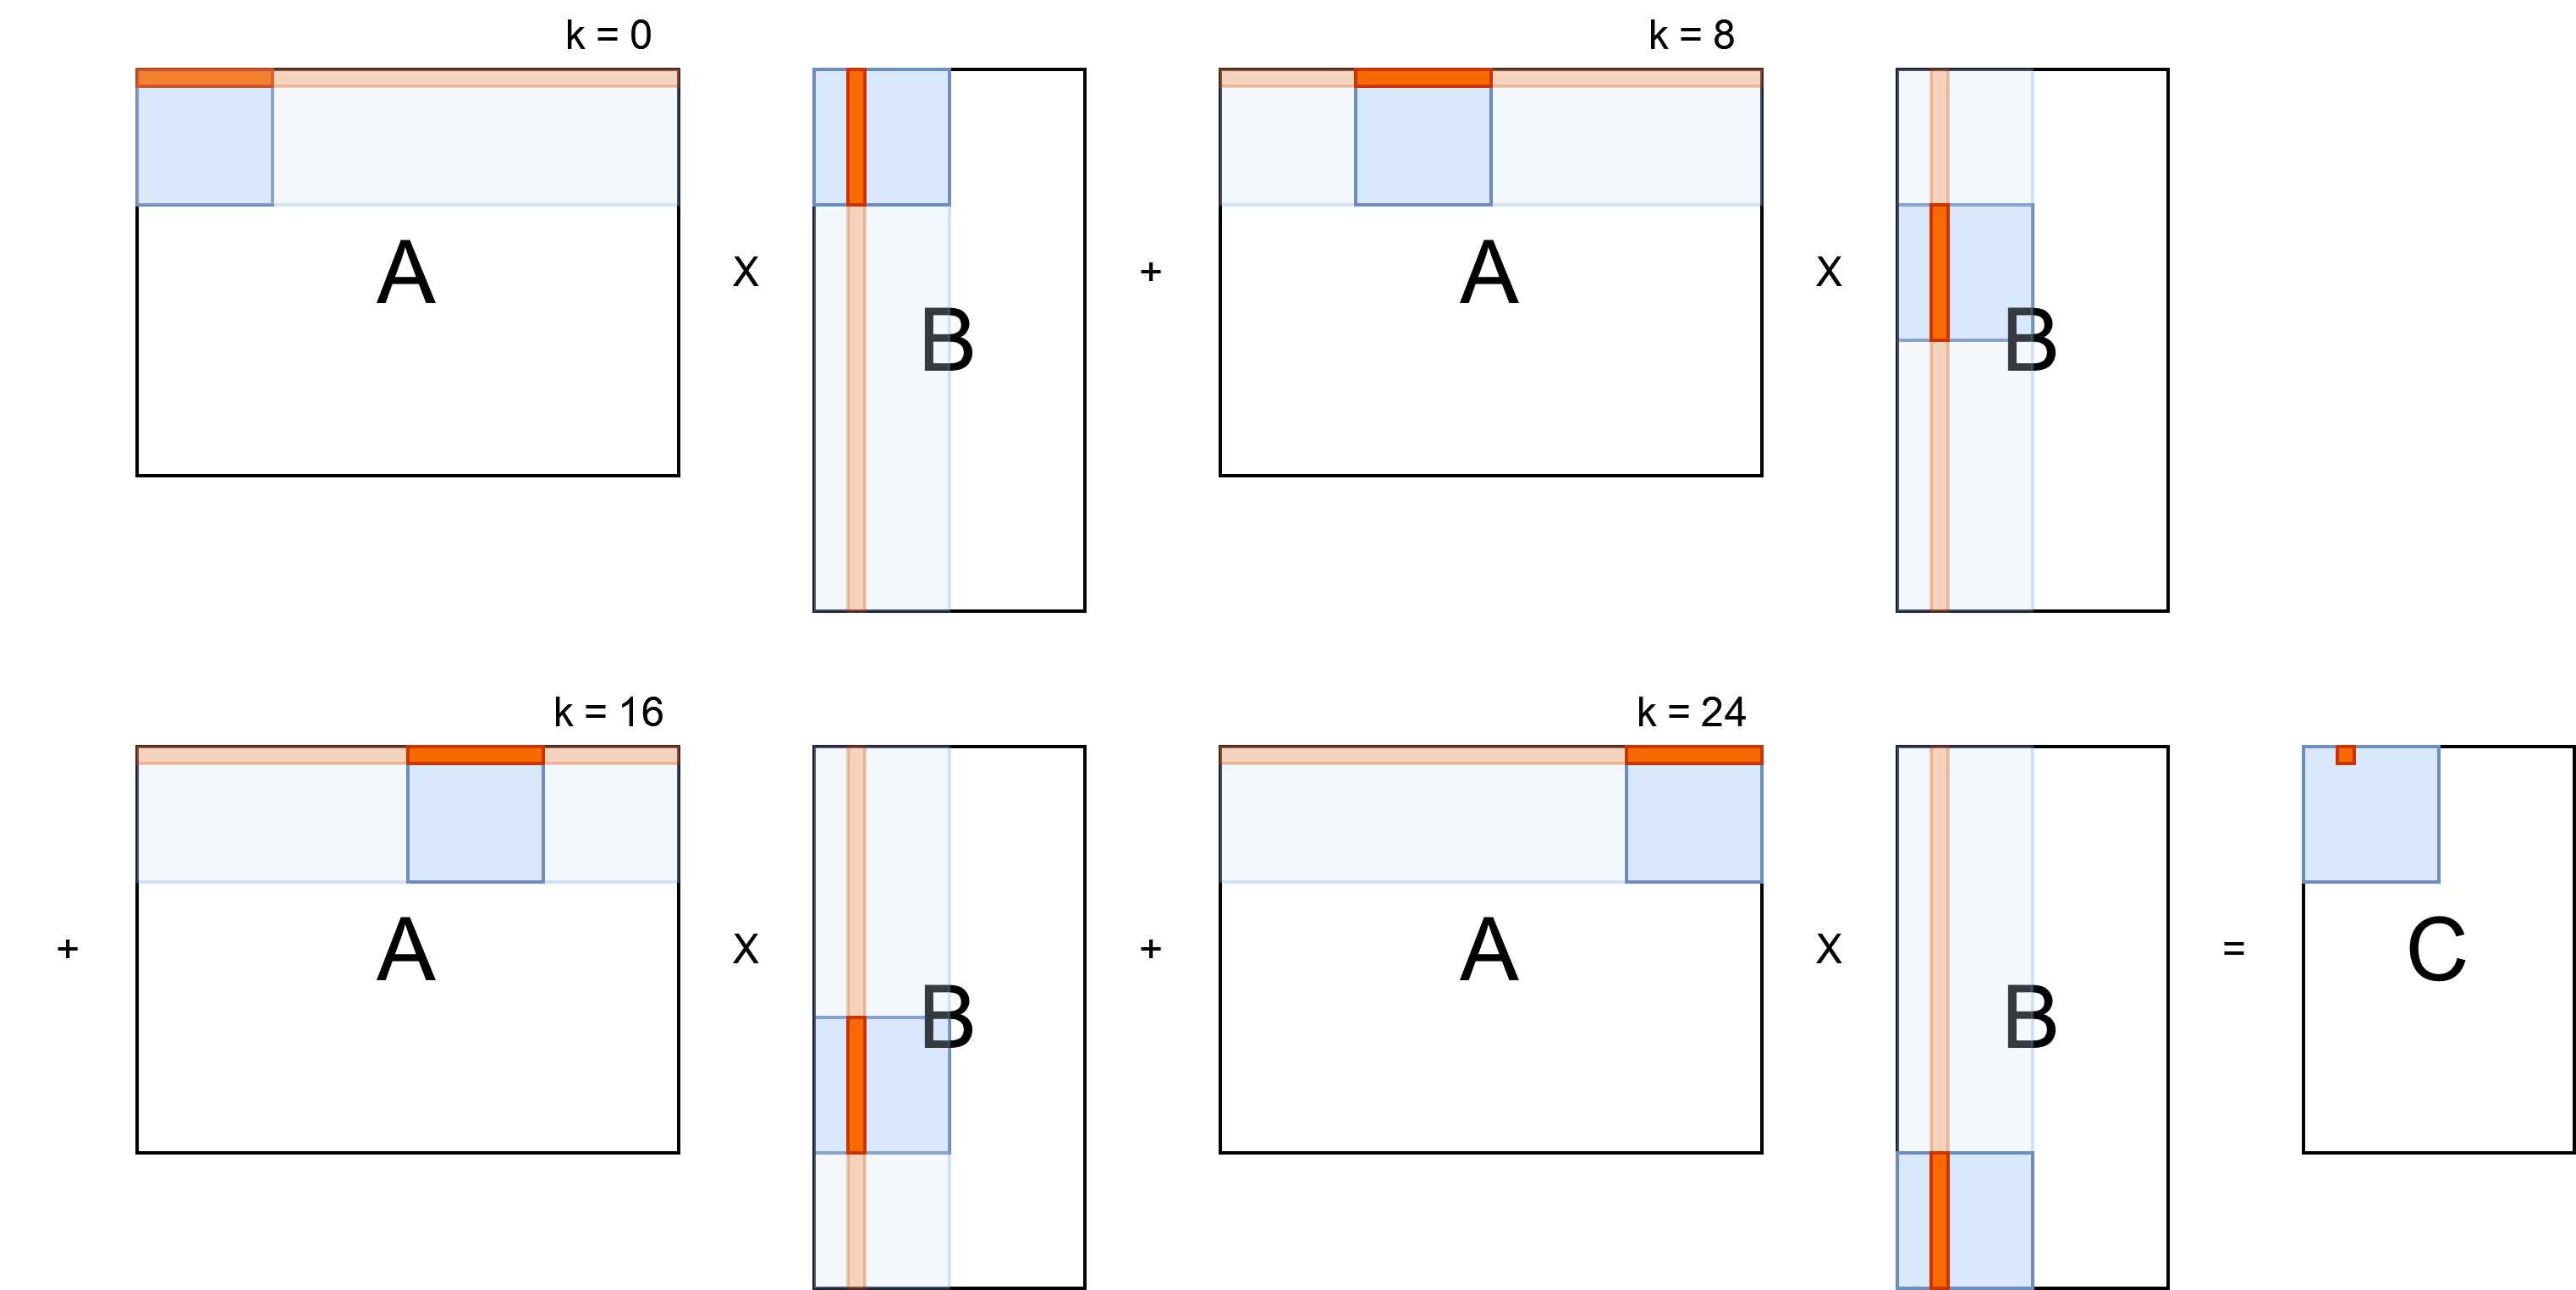
\includegraphics[width=\textwidth]{matmul/parallel_matmul8.png}
  \caption{Visualization of the vectorized matrix multiplication algorithm. With one run of the $k$-loop, we compute one $8\times8$ submatrix of $C$ (marked in blue). The orange cells depict the calculation of a single element of $C$.}
  \label{fig:vectorizedmatrixmultiplication}
\end{figure}

\subsubsection{Handling non-multiples of eight}
The algorithm in Algorithm~\ref{alg:vectorizedmatrixmultiplication} only works for matrices of which the dimensions are multiples of eight. Unfortunately, MEDS uses matrices of which the dimensions are usually not multiples of eight. To solve this problem, there are various approaches that we can take. An easy solution is to pad the matrices such that the dimensions become multiples of eight, but this would require additional memory and, if performed dynamically, additional computation time.

Our solution to this problem is threefold, as three dimensions can be non-multiples of eight: $m$, $o$, and $n$. We handle each of these dimensions separately.
\begin{itemize}
  \item \textbf{Dimension $m$}:\\
        When $m$ is not a multiple of eight, we can use the normal approach until we reach the last multiple of eight. After this, when loading the submatrix of $A$, we load an $(m \bmod 8) \times 8$ submatrix. Additionally, we only compute the dot products and store the results for the $m \bmod 8$ rows of $C$ that are required.
  \item \textbf{Dimension $o$}:\\
        When $o$ is not a multiple of eight, we can use the normal approach until we reach the last multiple of eight. After this, when loading the submatrix of $B$, we load an $8 \times (o \bmod 8)$ submatrix. The remaining lanes in the NEON registers containing $B_i$ are set to 0, making sure no incorrect values are added to $C$. When storing the results, we store only the first $o \bmod 8$ columns of $C$.
  \item \textbf{Dimension $n$}:\\
        When $n$ is not a multiple of eight, we can use the normal approach until we reach the last multiple of eight. After this, we load only an $8 \times (n \bmod 8)$ submatrix of $A$ and an $(n \bmod 8) \times 8$ submatrix of $B$. When computing $C_i$, we skip the last $8 - (n \bmod 8)$ multiplications and additions.
\end{itemize}
It is also possible for multiple of these dimensions to be non-multiples of eight at the same time. In this case, we can combine the approaches described above. In a few cases where the remaining number of rows or columns is less than eight but at least four, we can use 4-way vectorized instructions for a very small extra speedup.

\subsubsection{Implementation}
The actual implementation of Algorithm~\ref{alg:vectorizedmatrixmultiplication} combined with the handling of non-multiples can be done in multiple ways. As the resulting algorithm becomes quite complex, we figured that the C compiler might not be able to optimize the code as well as we can. Therefore, we have decided to implement a Python script\footnote{\url{https://github.com/MeItsLars/MEDS-ARMv8-optimization-thesis/blob/main/opt-low-level/src/asm/matmul/generate\_matmul\_asm.py}} that generates optimized ARMv8 assembly code. The script generates a specialized assembly function for each set of input dimensions that is used in MEDS.

\subsubsection{Minimum cycle bound}
To understand the performance of our optimized matrix multiplication algorithm, we need to find a minimum bound on the number of cycles that the algorithm will take to execute. To do this, we establish a minimum bound on the number of instructions that the algorithm uses.

A very crude minimum cycle bound on the naive algorithm (see Algorithm~\ref{alg:medsmatrixmultiplication}) can be established by counting the number of arithmetic operations required:
\begin{itemize}
  \item $m \cdot o \cdot n$ multiplications and additions;
  \item $m \cdot o$ modulo operations.
\end{itemize}
The `multiply-accumulate' operation is a single instruction on ARMv8, and modular reduction can be done in five instructions (see Section~\ref{sec:barrettreduction}). This means that we can establish a minimum bound of $m \cdot o \cdot n + m \cdot o \cdot 5$ on the number of arithmetic instructions required for the naive algorithm. Any algorithm that follows this structure will require at least this number of instructions to execute, divided by the parallelization factor of that algorithm. In the case of the vectorized algorithm, this factor is eight.

A more accurate minimum cycle bound can be established by looking at the number of instructions required for the vectorized algorithm (see Algorithm~\ref{alg:vectorizedmatrixmultiplication}). This algorithm obtains a speedup because of two factors:
\begin{itemize}
  \item The NEON unit can perform operations in parallel.
  \item As we compute the result for an $8\times8$ submatrix of $C$, we can use the same input value eight times, reducing the number of loads required.
\end{itemize}
The vectorized algorithm loads and later re-loads the same values multiple times. It is hard to account for this in a minimum cycle bound, as various implementations of the algorithm might require more or less loads. Therefore, we establish a minimum cycle bound based on the idea that we have infinite registers and need to load and store all required values only once. The number of instructions required for the vectorized algorithm can then be calculated as follows:
\begin{itemize}
  \item $\frac{1}{8}m \cdot \frac{1}{8}n \cdot 8$ loads of $A$;
  \item $\frac{1}{8}o \cdot \frac{1}{8}n \cdot 8$ loads of $B$;
  \item $\frac{1}{8}m \cdot \frac{1}{8}o \cdot \frac{1}{8}n \cdot 8 \cdot 8 \cdot 2$ multiply-accumulate operations;
  \item $\frac{1}{8}m \cdot \frac{1}{8}o \cdot 8 \cdot 2$ reductions;
  \item $\frac{1}{8}m \cdot \frac{1}{8}o \cdot 8$ stores of $C$.
\end{itemize}
Given that reduction takes five cycles and the other operations take one cycle, we establish the following minimum cycle bound:
\[
  % \frac{1}{8}m \cdot \frac{1}{8}o \cdot \frac{1}{8}n \cdot 8 \cdot (1 + 1 + 8 \cdot 2) + \frac{1}{8}m \cdot \frac{1}{8}o \cdot 8 \cdot (1 + 5 \cdot 2) = mo\left(\frac{9}{32}n + \frac{11}{8}\right)
  \frac{1}{8}mn + \frac{1}{8}on + \frac{1}{4}mon + \frac{1}{4}mo \cdot 5 + \frac{1}{8}mo = \frac{1}{4}mno + \frac{1}{8}mn + \frac{11}{8}mo + \frac{1}{8}no
\]
% \frac{1}{64}mo(18n + 88)

\subsection{Matrix systemizer}
\label{sec:matrixsystemizer}
The matrix systemizer function is the second most time-consuming function in MEDS, taking up about 9\% of the total number of cycles for key generation and 11\% of the total number of cycles for signing and verification. The function is responsible for the task of systemizing a matrix $A \in \mathbb{F}_{4093}^{m \times n}$ over the finite field $\mathbb{F}_{4093}$ into a systemized matrix of REF' or RREF' form (see Section~\ref{sec:systemizer}).

\subsubsection{Complexity analysis}
\label{sec:matrixsystemizercomplexity}
We analyze the complexity of the the matrix systemizer algorithm used in the reference implementation (see Algorithm~\ref{alg:systemizer}). We first consider the basic algorithm where $r_\text{max} = m$ and \texttt{do\_swap} and \texttt{do\_backsub} are set to false. We can then compute the complexity of the algorithm as follows:

\resizebox{\textwidth}{!}{
  \begin{minipage}{\textwidth}
    \begin{align*}
       & \sum_{r=0}^{m-1} \left( \sum_{r_2=r+1}^{m-1} \sum_{c=r}^{n-1} \mathcal{O}(1) + \mathcal{O}(1) + \sum_{c=r}^{n-1} \mathcal{O}(1) + \sum_{r_2=r+1}^{m-1} \sum_{c=r}^{n-1} \mathcal{O}(1) \right)                      \\
       & = 2 \cdot \left( \sum_{r=0}^{m-1} \sum_{r_2=r+1}^{m-1} \sum_{c=r}^{n-1} \mathcal{O}(1)\right) + \left( \sum_{r=0}^{m-1} \sum_{c=r}^{n-1} \mathcal{O}(1) \right) + \left( \sum_{r=0}^{m-1} \mathcal{O}(1) \right)    \\
       & = 2 \cdot \left( \sum_{r=0}^{m-1} \mathcal{O}((m-r-1)(n-r)) \right) + \left( \sum_{r=0}^{m-1} \mathcal{O}(n-r) \right) + \mathcal{O}(m)                                                                             \\
       & = 2 \cdot \left( \sum_{r=0}^{m-1} \mathcal{O}(mn - mr - nr + r^2 - n + r) \right) + \left( \sum_{r=0}^{m-1} \mathcal{O}(n-r) \right) + \mathcal{O}(m)                                                               \\
       & = \mathcal{O} \left( mn \sum_{r=0}^{m-1} 1 - m \sum_{r=0}^{m-1} r - n \sum_{r=0}^{m-1} r + \sum_{r=0}^{m-1} r^2 - n \sum_{r=0}^{m-1} 1 + \sum_{r=0}^{m-1} r + n \sum_{r=0}^{m-1} 1 - \sum_{r=0}^{m-1} r + m \right) \\
       & = \mathcal{O} \left( mn \cdot m - m \cdot \frac{(m-1)m}{2} - n \cdot \frac{(m-1)m}{2} + \frac{(m-1)m(2m-1)}{6} + m \right)                                                                                          \\
       & = \mathcal{O} \left( m^2n - \frac{m^3 - m^2}{2} - \frac{m^2n - mn}{2} + \frac{2m^3 - 3m^2 + m}{6} + m \right)                                                                                                       \\
       & = \mathcal{O} \left( m^2n - \frac{m^3}{2} + \frac{m^2}{2} - \frac{m^2n}{2} + \frac{mn}{2} + \frac{2m^3}{6} - \frac{3m^2}{6} + \frac{m}{6} + m \right)                                                               \\
       & = \mathcal{O} (m^2n)
    \end{align*}
  \end{minipage}
}

We can use arithmetic series to replace sums with closed-form expressions. In the final step, as $n \geq m$ and therefore $m^2n \geq m^3$, we find that the complexity of the basic algorithm is $\mathcal{O}(m^2n)$.

We consider the changes that the three optional features of the algorithm bring to the complexity:
\begin{itemize}
  \item Using $r_\text{max}$ will change the dimensions of the outer loop of the algorithm to $r_\text{max}$ instead of $m$. This will change the complexity of the algorithm to $\mathcal{O}(r_\text{max}mn)$. As $r_\text{max}$ is only ever $m$ or $m-1$ in MEDS, this has no drastic effect on the complexity of the algorithm.
  \item When \texttt{do\_swap} is set to true, an additional loop is added to the algorithm which adds the following complexity:
        \begin{align*}
           & \left( \sum_{r=0}^{m} \sum_{r_2=r+1}^{m} \mathcal{O}(1) \right) + \left( \sum_{r=0}^{m} \sum_{i=0}^{r} \mathcal{O}(1) \right)
        \end{align*}
        Following a similar approach as above, we find that this results in a complexity of $\mathcal{O}(m^2)$, which does not change the complexity of the algorithm.
  \item When \texttt{do\_backsub} is set to true, we perform another triple-nested loop to perform back substitution. This loop has the following complexity:
        \begin{align*}
           & \left( \sum_{r=0}^{m} \sum_{r_2=0}^{r} \mathcal{O}(1) \right) + \left( \sum_{r=0}^{m} \sum_{r_2=0}^{r} \sum_{c=m}^{n} \mathcal{O}(1) \right)
        \end{align*}
        Again, following a similar approach as above, we find that this results in a complexity of $\mathcal{O}(m^2 + m^2n - m^2) = \mathcal{O}(m^2n)$, which does not change the complexity of the algorithm.
\end{itemize}
From this, we can conclude that the complexity of the matrix systemizer algorithm is $\mathcal{O}(m^2n)$.

\subsubsection{Optimization}
\label{sec:matrixsystemizeroptimization}
We optimize the matrix systemizer algorithm by applying vectorization to the loops in the algorithm. Contrary to the matrix multiplication algorithm, we cannot easily parallelize the main $r$-loop in the algorithm, as the starting values of subloops depend on the (changing) value of $r$. This structure makes parallelization over the $r$-loop impossible. Instead, we optimize each inner loop separately by applying a parallelization technique tailored to the specific inner loop.

For all nested loops, we apply parallelization to the innermost loop. In the systemizer algorithm, this loop is always the easiest to parallelize, as it accesses matrix elements that are stored sequentially in memory. Each input matrix element is stored in a 12-bit field element, which fits into a 16-bit register. This means that we can compute 8 elements at the same time using 128-bit NEON registers.

Unfortunately, we are unable to use a full 8-way vectorization for all loops, as the algorithm uses multiplication operations. When multiplying two 16-bit values, the result is a 32-bit value, of which we cannot store eight in a 128-bit NEON register. We can work around this issue by using the \texttt{umull} instruction to multiply the lower four 16-bit values of two registers and the \texttt{umull2} instruction to multiply the upper four 16-bit values of two registers. After reducing both results, we can use the \texttt{uzp1} operation to combine the results back into a single 128-bit register.

\subsubsection{Handling non-multiples of eight}
\label{sec:matrixsystemizernonmultiples}
The inner loops that we are optimizing usually do not loop over a dimension that is a multiple of eight. To handle this, we use the following approach:
\begin{enumerate}
  \item While at least eight elements are left to process, use the 8-way vectorization approach;
  \item After this, if there are at least four elements left to process, use one iteration of a 4-way vectorized approach;
  \item After this, use a non-vectorized approach for any remaining elements (maximum 3).
\end{enumerate}

\subsubsection{Implementation}
As with the matrix multiplication algorithm, the resulting systemizer algorithm becomes quite complex. Although it can be implemented with NEON intrinsics, we opted for the faster approach of generating optimized ARMv8 assembly code using a Python script.\footnote{\url{https://github.com/MeItsLars/MEDS-ARMv8-optimization-thesis/blob/main/opt-low-level/src/asm/systemizer/generate\_systemizer\_asm.py}} The script generates a specialized assembly function for each set of input dimensions that is used in MEDS.

\subsubsection{Minimum cycle bound}
Finding a minimum cycle bound for the optimized systemizer algorithm is very similar to determining its complexity. As we can follow the same structure as in Section~\ref{sec:matrixsystemizercomplexity}, we omit some of the steps taken and refer the reader to that section for a more detailed explanation. As with matrix multiplication, we assume infinite registers and that all values are loaded and stored only once.

For the basic algorithm, the number of instructions required is as follows:
\begin{itemize}
  \item $r_\text{max} \cdot n \cdot \frac{1}{8}$ loads of $A$;
  \item $\sum_{r=0}^{r\_\text{max}-1} \sum_{r_2=r+1}^{m-1} \sum_{c=r}^{n-1} \frac{1}{8}$ add, bitwise AND, and freeze instructions (first inner loop);
  \item $\sum_{r=0}^{r\_\text{max}-1} 1$ finite field inversions;
  \item $\sum_{r=0}^{r\_\text{max}-1} \sum_{c=r}^{n-1} (\frac{1}{8} \cdot 2)$ multiply and reduce instructions (normalize loop);
  \item $\sum_{r=0}^{r\_\text{max}-1} \sum_{c=r}^{n-1} \frac{1}{8}$ combine instructions (normalize loop);
  \item $\sum_{r=0}^{r\_\text{max}-1} \sum_{r_2=r+1}^{m-1} \sum_{c=r}^{n-1} (\frac{1}{8} \cdot 2)$ multiply and reduce instructions (last inner loop);
  \item $\sum_{r=0}^{r\_\text{max}-1} \sum_{r_2=r+1}^{m-1} \sum_{c=r}^{n-1} \frac{1}{8}$ combine, add, subtract and freeze instructions (last inner loop);
  \item $r_\text{max} \cdot n \cdot \frac{1}{8}$ stores of $A$.
\end{itemize}

\pagebreak

Given that reduction takes five cycles, freezing takes three cycles, field inversion takes 115 cycles, and all other instructions take one cycle, combining these results using the same techniques as for the complexity analysis gives us the following minimum cycle bound for the basic algorithm:
\begin{align*}
   & \frac{1}{4} \cdot r_\text{max} \cdot n + 115 \cdot r_\text{max} + \frac{13}{8} \left( n \cdot r_\text{max} - \frac{(r_\text{max} - 1)r_{\text{max}}}{2} \right) \\
   & + \frac{23}{8} \left( mn \cdot r_\text{max} - m \cdot \frac{(r_\text{max} - 1)r_{\text{max}}}{2} - n \cdot \frac{(r_\text{max} - 1)r_{\text{max}}}{2} \right.   \\
   & \left. + \frac{(r_\text{max} - 1)r_{\text{max}}(2r_{\text{max}} - 1)}{6} - n \cdot r_\text{max} + \frac{(r_\text{max} - 1)r_{\text{max}}}{2} \right)
\end{align*}

When using the algorithm with \texttt{do\_swap} set to true, the following instructions are added to the minimum cycle bound:
\begin{itemize}
  \item $\sum_{r=0}^{r\_\text{max}-1} \sum_{r_2=r}^{m-1} \frac{1}{8}$ bitwise OR instructions (swap loop 1).
\end{itemize}
Following the same approach as above, using \texttt{do\_swap} adds the following value to the minimum cycle bound:
\begin{align*}
   & \frac{1}{8} \left( m \cdot r_\text{max} - \frac{(r_\text{max} - 1)r_{\text{max}}}{2} \right)
\end{align*}
\todo[inline]{Aaaaaaaaaaaaa ik snap er geen reet van}

When using the algorithm with \texttt{do\_backsub} set to true, the following instructions are added to the minimum cycle bound:
\begin{itemize}
  \item $\sum_{r=0}^{r\_\text{max}-1} \sum_{r_2=0}^{r-1} (\frac{1}{8} \cdot 2)$ multiply and reduce instructions (backsub middle loop);
  \item $\sum_{r=0}^{r\_\text{max}-1} \sum_{r_2=0}^{r-1} \frac{1}{8}$ combine, add, subtract, and freeze instructions (backsub middle loop);
  \item $\sum_{r=0}^{r\_\text{max}-1} \sum_{r_2=0}^{r-1} \sum_{c=r_\text{max}}^{n-1} (\frac{1}{8} \cdot 2)$ multiply and reduce instructions (backsub inner loop);
  \item $\sum_{r=0}^{r\_\text{max}-1} \sum_{r_2=0}^{r-1} \sum_{c=r_\text{max}}^{n-1} \frac{1}{8}$ combine, add, subtract, and freeze instructions (backsub inner loop).
\end{itemize}
Following the same approach as above, using \texttt{do\_backsub} adds the following value to the minimum cycle bound:
\begin{align*}
   & \frac{18}{8} \left( \frac{(r_\text{max} - 1)r_{\text{max}}}{2} \right) + \frac{18}{8} \left( n - r_\text{max} \right) \left( \frac{(r_\text{max} - 1)r_{\text{max}}}{2} \right)
\end{align*}

\subsection{Isometry derivation}
\label{sec:isometryderivation}
In all three operations of MEDS, the \texttt{solve\_opt} function is used to derive an isometry mapping $\phi = (\textbf{A} \in \mathbb{F}_q^{m \times m}, \textbf{B} \in \mathbb{F}_q^{n \times n})$ by constructing and solving a sparse system of linear equations, see Section~\ref{sec:derivingisometry}. The system that needs to be solved is constructed in a very specific way, which allows for a more efficient method of solving it (as opposed to using a more general algorithm like Gaussian elimination). Even though this more efficient method is used, the function still takes up a significant amount of time in the MEDS implementation.

Unfortunately, the function is also extremely large, with the reference code containing over 300 lines of code, making it very tedious to optimize the function as a whole. Instead, we profiled the function and found that the majority of the time of this function ($\pm 70~\%$) is spent on two relatively small triple-nested loops, while the remainder of the time ($\pm 30~\%$) is spent on all other parts of the function combined. Therefore, we focus on optimizing these two loops. Both loops have the same structure, so we only discuss the optimization of the first loop. This loop is shown in Algorithm~\ref{alg:systemsolving1}.

\begin{algorithm}
  \caption{Isometry derivation: time-consuming loop 1}
  \label{alg:systemsolving1}
  \lstinputlisting[language=C, style=CStyle]{code/solve_opt_loop1.c}
\end{algorithm}

\subsubsection{Complexity analysis}
\label{sec:isometryderivationcomplexity}
As mentioned in Section~\ref{sec:derivingisometry}, the complexity of the entire \texttt{solve\_opt} function is $\mathcal{O}(n^3)$. Analyzing the complexity of the two time-consuming loops specifically is trivial as they are both triple-nested loops that start and end at specific values. As can be derived from Algorithm~\ref{alg:systemsolving1}, the first loop has a complexity of:
\[
  \mathcal{O}((m-3)(m-1)m) = \mathcal{O}(3m - 4m^2 + m^3) = \mathcal{O}(m^3)
\]
Using the same approach, we find that the second time-consuming loop has a complexity of $\mathcal{O}(m^2n)$. Note that as $n = m + 1$ for the parameter sets that we consider, both loops are also $\mathcal{O}(n^3)$, which is the same as the complexity of the entire function.

\subsubsection{Optimization}
\label{sec:isometryderivationoptimization}
Fortunately, the loop structure of the time-consuming loops in the algorithm is very suitable for vectorization, meaning the C compiler might already have optimized the loops to a degree that we cannot improve upon.  Nevertheless, we try to optimize the loops by applying vectorization to the innermost loop, which always loops from $0$ to $\texttt{MEDS\_m}$ ($\texttt{MEDS\_n}$ for the second loop).

As the field elements are stored in 16 bits, we can compute eight elements at the same time using 128-bit NEON registers. Therefore, we compute the results for eight values of $r$ at the same time. We start by loading \texttt{tmp1}, which gives us a small problem, as these eight values are not stored sequentially in memory. Therefore, we load these values using normal load instructions and store them in a 128-bit NEON register. The remaining loads and stores can be done using vectorized instructions as those values are stored next to each other in memory.

As with the matrix systemizer, we are unable to use a full 8-way vectorization as the algorithm uses multiplication instructions, which result in 32-bit values. We apply the approach used in the matrix systemizer to work around this issue, see Section~\ref{sec:matrixsystemizeroptimization}.

\subsubsection{Handling non-multiples of eight}
Similar to the matrix systemizer function, the number of elements that need to be processed is usually not a multiple of eight. We use the same approach as with the matrix systemizer function to handle this issue (see Section~\ref{sec:matrixsystemizernonmultiples}), meaning we decrease the parallelization factor to four and one when there are not enough elements left to process.

\subsubsection{Implementation}
As the \texttt{solve\_opt} function is very large, we have decided not to implement the full function in ARMv8 assembly. This presented us with two options: either we use NEON intrinsics to parallelize the two time-consuming loops, or we write (a script that generates) ARMv8 assembly code for the two time-consuming loops. As the loops themselves are not very complex, we have decided to use NEON intrinsics to parallelize them, under the assumption that the assembly variant would not be much faster. Exploring the assembly-based optimization of these loops and the full function is left as future work, see Section~\ref{sec:futureworkopt}. The optimized C code with NEON intrinsics is quite elaborate, so we do not show it here. Instead, we refer to the code in the code repository.\footnote{\url{https://github.com/MeItsLars/MEDS-ARMv8-optimization-thesis/blob/main/opt-low-level/src/util.c}}

\subsubsection{Minimum cycle bound}
We establish a minimum cycle bound for the part of the \texttt{solve\_opt} function that we optimized: the two time-consuming loops. As they share the same structure, we show a general approach for establishing a minimum cycle bound for these loops, which we then apply to both loops to obtain a minimum cycle bound for the combined loops.

We call $x$ the number of iterations of the outermost loop, $y$ the number of iterations of the middle loop, and $z$ the number of iterations of the innermost loop. The minimum number of instructions for the triple-nested loop can be calculated as follows:
\begin{itemize}
  \item $x \cdot y$ loads of \texttt{tmp2} (it is loaded once per iteration of the innermost loop);
  \item $x \cdot y \cdot \frac{1}{8}z \cdot 8$ loads to load the 8 values of \texttt{tmp1};
  \item $x \cdot y \cdot \frac{1}{8}z \cdot 2$ multiplications and reductions to compute \texttt{prod\_low/high};
  \item $x \cdot y \cdot \frac{1}{8}z$ combinations of \texttt{prod\_low} and \texttt{prod\_high} to compute \texttt{prod};
  \item $x \cdot y \cdot \frac{1}{8}z$ loads to load \texttt{val};
  \item $x \cdot y \cdot \frac{1}{8}z$ additions, subtractions, and final reductions to compute \texttt{val};
  \item $x \cdot y \cdot \frac{1}{8}z$ stores of \texttt{val}.
\end{itemize}
Given that reductions take five cycles, freezes take three cycles, and all other operations take one cycle, we establish a minimum bound of $xy + xy \cdot \frac{1}{8}z \cdot (8 + 2 \cdot (1 + 5) + 1 + 1 + (1 + 1 + 3) + 1) = xy + \frac{28}{8}xyz$.

We have $x = m - 3, y = m - 1, z = m$ for loop 1 and $x = m - 2, y = m - 1, z = n$ for loop 2, where $m$ and $n$ are the values of the parameter set that is used (as shown in Table~\ref{tab:medsparametersets}). This gives us a total of $\frac{1}{8}(m-3)(m-1)(28m + 8)$ cycles for loop 1 and $\frac{1}{8}(m-2)(m-1)(28n + 8)$ cycles for loop 2, giving a combined total of $(m-3)(m-1)\left(\frac{7}{2}m + \frac{7}{2}n + 2\right)$ cycles.
% $\frac{1}{8}(m-3)(m-1)(28m + 28n + 16)$
\todo[inline]{Also state what the reduction is compared to the original}

\section{High-level optimization}
\label{sec:highleveloptimization}
The high-level optimization approach focuses on optimizing the MEDS implementation by parallelizing over the challenge space. MEDS uses a large number ($t$) of challenges and commitments in both signing and verification, which are all computed independently in a for-loop. Additionally, the computation for each commitment is the same for signing and very similar for verification. This means that we can parallelize the computation of the commitments for each challenge.

Before we can parallelize the computation of the commitments, we need to determine the number of commitments that we compute in parallel. The commitment computation is executed over $\mathbb{F}_{4093}$, which means that the field elements can be stored in 12 bits (which fits in a 16-bit register). This means that we can store up to eight field elements in a single 128-bit NEON register. From this, there are two possible parallelization factors we can consider.
\begin{enumerate}
  \item \textbf{Four-way parallelization}:\\
        Nearly all operations on field elements allow the values to stay in 16-bit registers. An exception is multiplication: the result of a multiplication of two field elements is a 24-bit value, which fits in a 32-bit register. This means that we can compute four multiplications at the same time using 128-bit NEON registers. Because of this limitation, we can choose to compute four commitments at a time.
  \item \textbf{Eight-way parallelization}:\\
        We can work around the multiplication limitation by using instructions such as \texttt{umull} and \texttt{umull2} to multiply the lower and upper four values (respectively) of two 128-bit NEON registers, after which we can reduce the results and combine them back into a single 128-bit register. Using this technique, we can compute eight commitments at the same time.
\end{enumerate}
Initially, we implemented the 4-way parallelization approach as it is easier to implement. However, we found that the 8-way parallelization approach is more efficient, as the extra parallelization far outweighs the small overheads introduced by the more complex implementation. Therefore, we focus on the 8-way parallelization approach in this section.

In this section, we discuss the high-level optimization of the MEDS implementation. We first discuss the alterations that need to be made to the underlying datatypes and supplemental algorithms to allow for high-level parallelization in Section~\ref{sec:highleveldataalgorithms}. Next, we discuss the actual parallelization of the commitment computations in Section~\ref{sec:commitmentparallelization}. Finally, we discuss the limitations of the high-level optimization approach in Section~\ref{sec:highlevellimitations}.

\subsection{Parallelization of datatypes and supplemental algorithms}
\label{sec:highleveldataalgorithms}
In the reference implementation of MEDS, the main datatypes used are defined as follows:
\begin{samepage}
  \begin{verbatim}
  #define GFq_t uint16_t
  #define pmod_mat_t GFq_t
\end{verbatim}
\end{samepage}
These two datatypes represent a field element and a matrix element, respectively. Matrices are stored as one-dimensional arrays in row-major order and are passed to functions using pointers to a \texttt{pmod\_mat\_t}.

To parallelize the algorithms that use these datatypes, we adjust the datatypes such that they represent multiple field/matrix elements at the same time. In our implementation, we add a \texttt{vec\_16x8.h} file\footnote{\url{https://github.com/MeItsLars/MEDS-ARMv8-optimization-thesis/blob/main/opt-high-level/include/vec\_16x8.h}} containing these new datatypes, which are defined as follows:
\begin{samepage}
  \begin{verbatim}
  #define GFq_vec_t uint16x8_t
  #define pmod_mat_vec_t GFq_vec_t
\end{verbatim}
\end{samepage}
These two datatypes represent eight field elements and eight matrix elements, respectively. By passing these datatypes to a modified version of each function, we can compute the function output for eight commitments at the same time.

Additionally, we define a wide range of functions that operate on these vectorized datatypes in the \texttt{vec\_16x8.h} file. Examples of such definitions include:
\begin{samepage}
  \begin{verbatim}
  #define ADD_VEC(a, b) vaddq_u16(a, b)
  #define MUL_VEC_LOW(a, b) vmull_u16(vget_low_u16(a), 
                                      vget_low_u16(b))
  #define MUL_VEC_HIGH(a, b) vmull_high_u16(a, b)
  #define OR_VEC(a, b) vorrq_u16(a, b)
\end{verbatim}
\end{samepage}
The main advantage of this approach is that the entire high-level-optimized MEDS implementation can easily be converted to use a different CPU architecture (that supports vectorization) such as AVX512~\cite{intel-avx512} simply by changing the definitions in the \texttt{vec\_16x8.h} file.

\subsubsection{Supplemental algorithms}
\label{sec:suppalgorithmsparallelization}
To parallelize the commitment computations, we need to modify the supplemental algorithms that are used in the MEDS implementation. In the reference implementation, these algorithms perform operations for matrices or values that belong to a single commitment. We need to modify these algorithms such that they can perform operations for multiple commitments at the same time. The following algorithms need to be modified:
\begin{enumerate}
  \item \textbf{Matrix multiplication}: \texttt{pmod\_mat\_mul}\\
        Responsible for multiplying two matrices over the finite field $\mathbb{F}_{4093}$.
  \item \textbf{Matrix systemizer}: \texttt{pmod\_mat\_syst\_ct\_partial\_swap\_backsub}\\
        Responsible for converting a matrix into a systematic form (Algorithm~\ref{alg:systemizer}, Appendix~\ref{app:supplementalalgs}).
  \item \textbf{Field inversion}: \texttt{GF\_inv}\\
        Responsible for inverting an element over the finite field $\mathbb{F}_{4093}$.
  \item \textbf{Matrix inversion}: \texttt{pmod\_mat\_inv}\\
        Responsible for inverting a matrix over the finite field $\mathbb{F}_{4093}$.
  \item \textbf{Isometry derivation}: \texttt{solve\_opt}\\
        Responsible for deriving an isometry mapping $\phi$ by constructing and solving a sparse system of linear equations over the finite field $\mathbb{F}_{4093}$.
  \item \textbf{Applying the $\pi$ function}: \texttt{pi}\\
        Responsible for applying the $\pi$ function (Algorithm~\ref{alg:medspifunction}, Appendix~\ref{app:supplementalalgs}) to a pair of matrices.
  \item \textbf{Applying the SF function}: \texttt{SF}\\
        Responsible for applying the SF function (Algorithm~\ref{alg:medssffunction}, Appendix~\ref{app:supplementalalgs}) to a matrix.
\end{enumerate}
Each of these algorithms will be modified to work with the vectorized datatypes defined in the \texttt{vec\_16x8.h} file. These algorithms will then be plugged into the MEDS implementation, which will be modified to compute multiple commitments at the same time.

To give a brief overview of the modifications that need to be made to these algorithms, we provide an example for the matrix multiplication algorithm. The reference matrix multiplication algorithm is shown in Algorithm~\ref{alg:medsmatrixmultiplication} (Appendix~\ref{app:supplementalalgs}). The C code for this algorithm is shown in Algorithm~\ref{alg:medsmatrixmultiplicationc}. The modified matrix multiplication algorithm is shown in Algorithm~\ref{alg:medsmatrixmultiplicationvec}. Both algorithms are slightly simplified for the sake of readability.

\begin{algorithm}
  \caption{Matrix multiplication (non-vectorized)}
  \label{alg:medsmatrixmultiplicationc}
  \lstinputlisting[language=C, style=CStyle]{code/matrix_multiplication.c}
\end{algorithm}

\begin{algorithm}
  \caption{Matrix multiplication (vectorized for eight commitments)}
  \label{alg:medsmatrixmultiplicationvec}
  \lstinputlisting[language=C, style=CStyle]{code/matrix_multiplication_vec.c}
\end{algorithm}

\pagebreak

As can be seen from the code, the vectorized version is essentially the same as the non-vectorized version, but with certain operations altered so they work with the vectorized datatypes and functions defined in the \texttt{vec\_16x8.h} file and thus perform 8 computations in
parallel. The same approach is used for all other supplemental algorithms that require parallelization, their modified implementations can be found in the code repository.\footnote{\url{https://github.com/MeItsLars/MEDS-ARMv8-optimization-thesis/tree/main/opt-high-level/src}}

\subsection{Parallelization of commitment computations}
\label{sec:commitmentparallelization}
Using the modified datatypes and supplemental algorithms, we can parallelize the computation of the commitments in MEDS. As can be seen in the algorithms for both signing (Algorithm~\ref{alg:medssignoverview}) and verification (Algorithm~\ref{alg:medsverifyoverview}), the computation of the commitments is done in a for-loop that loops from $0$ to $t$. As the generation of a commitment can fail (for example, when a randomly generated matrix is not invertible), the generation of a particular commitment is done in a while loop that runs until the commitment is successfully generated. This is why the signing and verification code exhibits the following structure:
\begin{samepage}
  \begin{verbatim}
  // Initial definitions and loading
  for (int i = 0; i < t; i++) {
    while (1) {
      // Compute commitment
      if (commitment is computed) {
        break;
      }
    }
  }
  // Final operations
\end{verbatim}
\end{samepage}
This structure introduces a problem if we want to parallelize the computation of the commitments. We cannot simply parallelize the for-loop to use $\frac{t}{8}$ iterations, as the while loop might run for a different number of iterations for each commitment. Additionally, although the computation of two different commitments is independent, the computation of the same commitment (after a failure) is dependent on the previous computation of that commitment, as the seed for the random number generator is updated after each failure. This means that we also cannot parallelize the while-loop.

\subsubsection{Optimization}
\label{sec:commitmentparallelizationoptimization}
We can overcome the aforementioned problems by using a different approach to parallelize the commitment computations. Instead of finishing the computation for a commitment before moving on to the next, we start by running the first computation attempt for each commitment. If a computation fails, we store the necessary information to retry the computation later. After the first computation attempt for all commitments is done, we run the second computation attempt for all commitments that failed the first time. This process is repeated until all commitments are successfully computed. This approach is inspired by~\cite{IIS2023HighLevel}. It is suitable for parallelization and has the following structure:
\begin{samepage}
  \begin{verbatim}
  // Initial definitions and loading
  while (there are uncomputed/failed commitments) {
    // 1. Load data for next 8 uncomputed/failed commitments
    // 2. Compute these commitments in parallel
    // 3(a). Store results for successful commitments
    // 3(b). Store information for failed commitments
  }
  // Final operations
\end{verbatim}
\end{samepage}
Of course, this introduces some overhead, as steps 1 and 3 in the structure above cannot be parallelized and take slightly more time than their equivalent in the reference implementation. However, the parallelization of step 2 will result in a significant speedup, as the computation of the commitments itself is by far the most time-consuming part of the MEDS implementation.

\subsubsection{Verification}
For the signature verification algorithm, the same approach can be used with a few minor adjustments. The verification algorithm is shown in Algorithm~\ref{alg:medsverifyoverview}. As can be seen, the verification of a commitment can be done in two ways. If $h_i$ is not zero, we compute the isometry mapping based on the commitment that is contained in the signature. If $h_i$ is zero, we re-compute the isometry mapping in the same way as in the signing algorithm.

A key observation is that in both cases, the same matrix multiplication and isometry derivation algorithms are used, with the same dimensions and parameters. The only difference is the source of the matrices. This means that we can use the same parallelization approach described earlier, with a small change in the way the matrices are loaded. This is done separately for each matrix, which will bring a small overhead, but will still result in a significant speedup.

\subsection{Limitations}
\label{sec:highlevellimitations}
Theoretically, we should expect that this approach will result in a speedup factor of eight. However, there are a few important reasons that will prevent us from reaching this speedup factor:
\begin{enumerate}
  \item \textbf{Overhead}:\\
        As mentioned earlier, the parallelization approach introduces some overhead. This overhead is caused by the fact that we cannot parallelize the loading of the data and the storing of the results.
  \item \textbf{Memory bandwidth}:\\
        The parallelization approach will result in a much higher memory bandwidth usage, as the inputs and outputs of each supplemental algorithm are now 8 times larger. This implies that the inputs and outputs to supplemental algorithms will no longer fit in the L1 cache of the CPU, which will result in a larger amount of cache misses, causing a severe slowdown.
\end{enumerate}

\section{Bitstream filling}
\label{sec:bitstreamfilling}
After the commitments are computed, the resulting matrices are hashed, after which the hash output is converted into an array of $t$ challenges. The input to the hash function is an array of 8-bit unsigned integers. For the MEDS parameter sets that we consider, the matrix elements fit in 12 bits and are stored as 16-bit unsigned integers. This means that the 16-bit values need to be converted to 8-bit values before they can be hashed. Although this can be done by simply changing the pointer type (for C implementations), MEDS uses the more complex approach of only using the 12 least significant bits (which contain the field element) of each 16-bit value. These 12-bit values are concatenated into a bitstream which is then hashed.

The main advantage of this approach is that the number of 8-bit values that need to be hashed is reduced by a factor of $\frac{16}{12} = \frac{4}{3}$, lowering the number of calls to the hash function. However, it also comes with the disadvantage that the process of filling the bitstream is more complex and time-consuming than the alternative of changing the pointer type.

We discuss the optimization of the existing approach for filling the bitstream. The alternative approach of changing the pointer type is left as future work, see Section~\ref{sec:futureworkopt}.

The reference implementation\footnote{\url{https://github.com/MeItsLars/MEDS-ARMv8-optimization-thesis/blob/main/ref/src/bitstream.c}} for filling the bitstream is generalized to work with up to 32 bits per value and therefore has to keep track of and update the current bit position in the bitstream. This means that we can save some time by using a specialized approach for filling bitstreams with 12-bit values.

Our optimization relies on the observation that two 12-bit values can be converted to three 8-bit values (which are required by the hash function) using a few simple bitwise operations. A conceptual pseudocode implementation of this approach is shown in Algorithm~\ref{alg:bitstreamfillingalg}. The actual implementation\footnote{\url{https://github.com/MeItsLars/MEDS-ARMv8-optimization-thesis/blob/main/opt-low-level/src/meds.c}} is a bit more complex as the structure of the input data is different and it needs to handle the case where the number of values is not a multiple of two. The high-level variant\footnote{\url{https://github.com/MeItsLars/MEDS-ARMv8-optimization-thesis/blob/main/opt-high-level/src/vec\_16x8.c}} is also slightly different as it needs to parallelize this operation.

\begin{algorithm}
  \caption{Bitstream filling for 12-bit values}
  \label{alg:bitstreamfillingalg}
  \begin{algorithmic}[1]
    \State \textbf{Input:} $v$: array of $n$ 16-bit unsigned integers
    \State \textbf{Output:} $bs$: array of $\frac{3}{2}n$ 8-bit unsigned integers
    \State $bs \gets \text{empty array of size } \frac{3}{2}n$
    \State $i \gets 0$
    \For{$j \gets 0$ to $n$ in steps of 2}
    \State $v_1 \gets v[j]$
    \State $v_2 \gets v[j + 1]$
    \State $bs[i] \gets v_1 ~\&~ \texttt{0xFF}$
    \State $bs[i + 1] \gets (v_1 \gg 8) ~|~ ((v_2 ~\&~ \texttt{0xF}) \ll 4)$
    \State $bs[i + 2] \gets (v_2 \gg 4) ~\&~ \texttt{0xFF}$
    \State $i \gets i + 3$
    \EndFor
  \end{algorithmic}
\end{algorithm}

\section{Hash structure}
\label{sec:hashfunctionoptimization}
The result of the computation of each commitment is a large matrix. To convert these commitments into a set of challenges (as is required by the Fiat-Shamir structure, see Section~\ref{sec:fiatshamir}), the commitments are hashed (using the SHAKE256 XOF) into a single KECCAK state. This state is then converted into an array of $t$ challenges.

The commitment matrices are hashed sequentially, meaning that to hash commitment $i$, we are dependent on the hash output of commitment $i - 1$. The structure of this hashing process is depicted in Figure~\ref{fig:hashstructure}. In this figure, $\tilde{\textbf{G}}_i$ represents the commitment matrix for commitment $i$, converted such that it is stored in an array of $k(mn - k)$ unsigned 8-bit integers (see Section~\ref{sec:parametersets} for values of $m$, $n$, and $k$). $\textit{Hash}_1$ represents a call to SHAKE256, which in turn calls the Keccak-f[1600] permutation until the entire input array is absorbed. $s_i$ represents the intermediate KECCAK state after hashing commitment $i$, where $s_0$ is 0. The resulting state $s_t$ is used to generate the array of challenges.

\begin{figure}
  \centering
  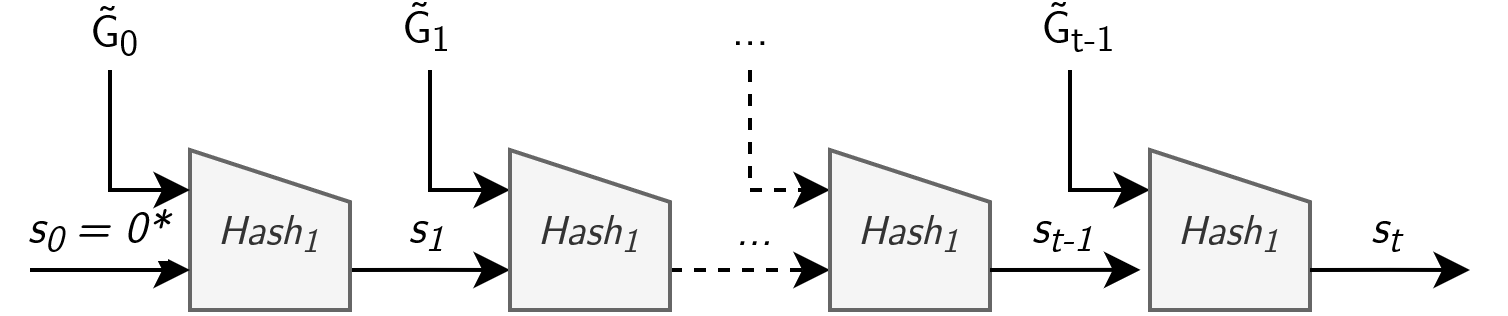
\includegraphics[width=\textwidth]{hash/hash_struct_seq.png}
  \caption{MEDS commitment hashing structure. $\tilde{\textbf{G}_i}$ represents the commitment matrix for commitment $i$, $\textit{Hash}_1$ represents a call to SHAKE256, and $s_i$ represents the intermediate KECCAK state after hashing commitment~$i$.}
  \label{fig:hashstructure}
\end{figure}

The hashing process for a single commitment is already quite computationally expensive. The number of bits to be hashed per commitment is $8 \cdot \lceil \frac{k(mn-k) \cdot b}{8} \rceil$, where $b$ is the number of bits required to store a field element. For MEDS-55520 (see Section~\ref{sec:parametersets}), this results in a value of $471648$. As SHAKE256 uses a rate of 1088 bits, this means that the hashing process for a single commitment requires $\lceil \frac{471648}{1088} \rceil = 434$ calls to the Keccak-f[1600] permutation (for MEDS-55520).

Additionally, the hashing process is not parallelizable because of the sequential structure of the process. The profiling results (see Section~\ref{sec:medsprofilingresults}) show that the hashing process takes up a little over 5\% of the total execution time of signing and verification, which makes it worthwhile to explore possible optimizations.

\subsection{Hash structure optimization}
There is little to no room for improvement in the actual SHAKE256 XOF, as it (and the underlying KECCAK permutation) is already widely studied and optimized. However, we can optimize the structure of the hashing process in such a way that we can compute the hashing result for multiple commitments in parallel. To do this, we need to alter the structure of the hashing process. This altered structure is depicted in Figure~\ref{fig:hashstructureopt}. In this structure, the hashing structure is split into two stages:
\begin{enumerate}
  \item \textbf{Stage 1}: $\textit{Hash}_1$\\
        In the first stage, the commitment matrices are hashed into a set of intermediate states $i_0, i_1, \ldots, i_{t-1}$ using the same $\textit{Hash}_1$ function as in the original structure. This stage can be parallelized, as the hashing of each commitment no longer depends on other commitments.
        \pagebreak
  \item \textbf{Stage 2}: $\textit{Hash}_2$\\
        In the second stage, we combine the intermediate states $i_0, i_1, \ldots, i_{t-1}$ into a single state $s_t$ that we can use to generate the array of challenges. We do this by repeatedly applying the $\textit{Hash}_2$ function (which also calls SHAKE256) to the intermediate states and the running state $s$. This stage is once again sequential, but it only requires $t$ calls to the Keccak-f[1600] permutation.
\end{enumerate}
The resulting structure introduces a small amount of overhead, as stage 2 requires $t$ additional calls to the Keccak-f[1600] permutation. However, as stage 1 can now be parallelized, the overall execution time of the hashing process is expected to decrease.

\begin{figure}
  \centering
  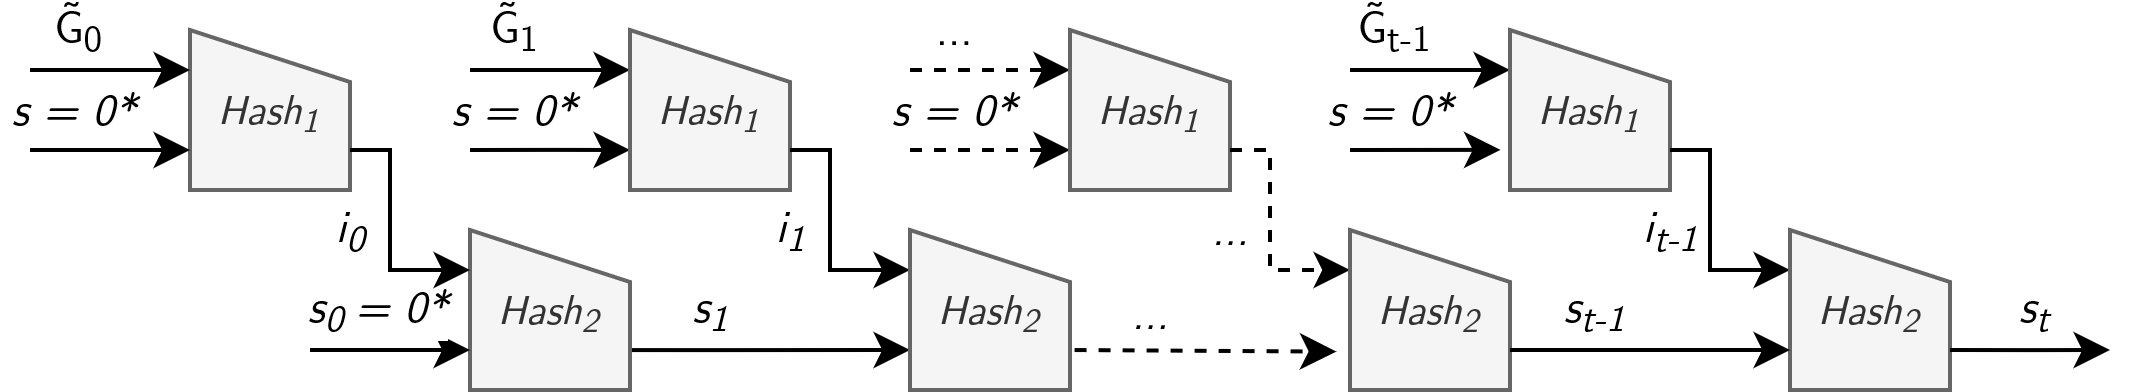
\includegraphics[width=\textwidth]{hash/hash_struct_par.png}
  \caption{Optimized MEDS commitment hashing structure. $\tilde{\textbf{G}_i}$ represents the commitment matrix for commitment $i$, $\textit{Hash}_1$ and $\textit{Hash}_2$ represent calls to SHAKE256, and $i_i$ and $s_t$ represent intermediate and final KECCAK states, respectively.}
  \label{fig:hashstructureopt}
\end{figure}

Unfortunately, the final state $s_t$ that the optimized structure generates is different from the final state that the original structure generates. This means that the resulting challenges will also be different between the two structures, meaning that the optimized and reference implementations are not compatible with each other. Therefore, we leave this optimized hash structure as a suggested change to the MEDS scheme.

\subsection{Implementation}
The implementation of the optimized hash structure into the MEDS implementation is trivial and requires only one important detail: a parallelized version of SHAKE256, optimized for the ARMv8 architecture. The extended KECCAK code package~\cite{xkcp} does not contain vectorized implementations of the Keccak-f[1600] permutation for ARMv8 (only for ARMv7). Fortunately, recent research by Becker and Kannwischer~\cite{becker2022hybrid} has resulted in a large set of optimized and vectorized implementations of the Keccak-f[1600] permutation for ARMv8 and various extensions of the ARMv8 architecture.

We have benchmarked these implementations on the Cortex-A72 and found that the \texttt{keccak\_f1600\_x4\_hybrid\_asm\_v3p}\footnote{\url{https://gitlab.com/arm-research/security/pqax/-/blob/master/asm/manual/keccak\_f1600/keccak\_f1600\_x4\_hybrid\_asm\_v3p.s}} optimized permutation (which can process 4 states in parallel) requires the lowest amount of cycles per state permutation. As the number of challenges $t$ is a multiple of 4 for all MEDS parameter sets that we consider, this means that we can easily plug this optimized permutation into the new hash structure.

\section{Non-constant-time implementations}
\label{sec:nonconstanttime}
To prevent timing and cache-based side-channel attacks (see Section~\ref{sec:optimizingcrypto}), the MEDS implementation must be constant-time. However, this is only the case for the key generation and signing phases of MEDS. The verification phase is not required to be constant-time, as it operates only on public data. This means that we can use non-constant time code for the verification phase. In this section, we list the functions that can be optimized using non-constant time implementations. The implementation of each optimization is slightly different for the low-level and high-level approaches, but the idea is the same.

\subsection{Finite field inversion}
MEDS requires the inversion of field elements over the finite field $\mathbb{F}_{4093}$. The constant-time algorithm used in the reference implementation utilizes an optimal addition chain based on the inversion approach of Fermat's Little Theorem, which uses 115 instructions. However, as the number of possible field elements is limited to 4093, we can precompute the inverse of each field element and store it in a lookup table. This allows us to invert a field element simply by executing an array lookup, which takes only a few instructions to execute.

\subsection{Matrix systemizer}
In the matrix systemizer (shown in Algorithm~\ref{alg:systemizer}), the algorithm spends some time making sure the leading coefficient of each row is nonzero (it almost always is). As the implementation is constant time, this entire process is executed even if the leading coefficient is already nonzero. In a non-constant time implementation, we add a check to see if the leading coefficient is zero, and if it is not, skip the entire process of making it nonzero.

\chapter{Results}
\label{ch:results}
In this chapter, we present the results of the optimizations that we have performed on the MEDS implementation. We compiled the code using gcc (Debian 12.2.0-14) 12.2.0 with the \texttt{-O3} optimization flag. In all tables and figures, the numbers shown represent the number of cycles, kilocycles (KCycles, 1 KCycle = 1 thousand cycles), or megacycles (MCycles, 1 MCycle = 1 million cycles) that the respective algorithm or function took to execute.

We first look at the performance results of the three algorithms that were optimized specifically for the low-level approach in Section~\ref{sec:resultslowlevel}. After that, we look at the post-optimization profiling results of the functions that originally took up the most time in the MEDS implementation in Section~\ref{sec:profilingoptimizations}. Following this, we look at the overall performance results of all three MEDS parameter sets for both the reference implementation, low-level optimized implementation, and high-level optimized implementation in Section~\ref{sec:overallperformance}. Finally, we compare the performance of the optimized MEDS implementation to other state-of-the-art signature schemes in Section~\ref{sec:comparison}.

\section{Low-level optimizations}
\label{sec:resultslowlevel}
In our low-level optimization approach (see Section~\ref{sec:lowleveloptimization}), we optimized matrix multiplication, the matrix systemizer, and isometry derivation. For each of these functions, we established a lower bound on the number of cycles that the (optimized part of the) function should take to execute. The calculated lower bounds are applicable to the algorithms that we used for the optimizations. Using a different algorithm might result in a different lower bound.

To determine how close we got to our calculated bound, we benchmarked the optimized functions for parameter set MEDS-55520. Together with the cycle count of the original function and the calculated minimum bound for each function (part), this gives us an understanding of how close we got to the optimal performance of the function (with the specific algorithm that we used). The results for these optimizations are shown in Table~\ref{tab:lowleveloptimizationresults}. Each benchmark result was obtained by running that function 128 times and taking the minimum of the timing results.

\begin{table}
  \centering
  \caption{Results of low-level algorithm optimizations for parameter set MEDS-55520. `Cycles' represents the number of cycles that the reference (Ref.) or optimized (Opt.) function (part) took to execute. `Bound' represents the lower bound (as calculated in the relevant section in Chapter~\ref{ch:methodology}) on the number of cycles that the function (part) should take to execute. `Ratio' represents the ratio between the number of cycles that the optimized function (part) took to execute and the lower bound. For the Matrix Systemizer, the arguments (as explained in Section~\ref{sec:matrixsystemizer}) are represented by $^*$ (apply back substitution), $^{**}$ (apply systemizer to a limited number of rows), and $^{***}$ (swap columns to ensure non-zero leading coefficients).}
  \vspace{0.5em}
  \resizebox{\textwidth}{!}{
    %
    \begin{tabular}{lllR{1.35cm}R{1.2cm}R{1.2cm}r}
      \toprule
      \textbf{Function}                        & \multicolumn{2}{c}{\textbf{Input size}} & \textbf{Cycles}                & \textbf{Cycles} & \textbf{Bound} & \textbf{Ratio}        \\
                                               & \multicolumn{1}{c}{\textit{A}}          & \multicolumn{1}{c}{\textit{B}} & \text{(Ref.)}   & \text{(Opt.)}  &                &      \\
      \toprule
      Matrix Multiplication                    & $2 \times k$                            & $k \times k$                   & 6450            & 1348           & 744            & 1.81 \\
      Matrix Multiplication                    & $2 \times mn$                           & $mn \times k$                  & 226217          & 39234          & 22852          & 1.72 \\
      Matrix Multiplication                    & $k \times mn$                           & $mn \times k$                  & 3757155         & 489947         & 388488         & 1.26 \\
      Matrix Multiplication                    & $m \times n$                            & $n \times m$                   & 109556          & 15947          & 12969          & 1.23 \\
      Matrix Multiplication                    & $m \times n$                            & $n \times n$                   & 111334          & 16794          & 13350          & 1.26 \\
      Matrix Multiplication                    & $32 \times 32$                          & $32 \times 32$                 & 89725           & 10750          & 10624          & 1.01 \\
      \midrule
      Matrix Systemizer                        & $k \times k$                            &                                & 169141          & 95299          & 71438          & 1.33 \\
      Matrix Syst.                             & $k \times 2k$                           &                                & 292309          & 175155         & 170710         & 1.03 \\
      Matrix Syst. (bsub$^{*}$)                & $n \times 2n$                           &                                & 453498          & 292422         & 274242         & 1.07 \\
      Matrix Syst. (bsub$^{*}$)                & $m \times 2m$                           &                                & 407491          & 261331         & 251704         & 1.04 \\
      Matrix Syst. (bsub$^{*}$)                & $k \times 2k$                           &                                & 407583          & 261028         & 251704         & 1.04 \\
      Matrix Syst. (n-1$^{**}$) (bsub$^{*}$)   & $n \times 2m$                           &                                & 422529          & 269895         & 260463         & 1.04 \\
      Matrix Syst. (swap$^{***}$) (bsub$^{*}$) & $m-1 \times m$                          &                                & 190097          & 123796         & 73106          & 1.69 \\
      \midrule
      Isometry Derivation (part)               & $2 \times mn$                           &                                & 1142883         & 350909         & 249100         & 1.41 \\
      \bottomrule
    \end{tabular}
    %
  }
  \label{tab:lowleveloptimizationresults}
\end{table}

The results show that we were able to optimize the matrix multiplication function for the $32 \times 32$ case to within 2\% of the lower bound. This case is not used in MEDS, but we added it to show that the optimization works almost perfectly for matrices of which the dimensions are a multiple of 8. The other cases show that the optimization works fairly well for matrices with more than 8 rows and columns. These cases are unable to reach the lower bound because of the overhead of having to deal with dimensions that are not a multiple of 8, but the results are still very good. The worst case arises when one of the input matrices has only 2 rows. This makes sense, as we are unable to use full 8-way parallelization and therefore lose performance. The optimization of matrix multiplication for these cases might be improved by using a different approach to parallelization, which we leave as future work (see Section~\ref{sec:futureworkopt}).

When looking at the matrix systemizer, we see that we get very close to the lower bound for most cases. The exceptions are the cases where the matrix size is relatively small, which is to be expected. For these matrix sizes, the overhead of having to deal with dimensions that are not a multiple of 8 is relatively large, compared to the parallelization speedup.

Finally, we consider the isometry derivation function. The results show that we were able to optimize this function to within 41\% of the lower bound. This is a major improvement over the reference implementation, but it is still quite far from the lower bound. This can be attributed to the fact that we only optimized the two most time-consuming parts of the function. Furthermore, we used NEON intrinsics for the optimization, whereas an assembly implementation might have resulted in a larger speedup. We leave this as future work (see Section~\ref{sec:futureworkopt}).

\section{Profiling implementation variants}
\label{sec:profilingoptimizations}
The results of profiling the reference implementation were shown earlier in Section~\ref{sec:medsprofilingresults}. In this section, we profile the optimized implementations (both low-level and high-level) for parameter set MEDS-55520 to obtain an understanding of how much impact each optimization had. The relative results for the other two parameter sets are very similar and are therefore omitted. As the main goal of profiling does not revolve around getting accurate measurements but rather around understanding the relative performance of (functions within) the different implementations, we only ran one profiling iteration for each of the three algorithms. The profiling results, depicted in bar charts, are shown in Figure~\ref{fig:results_profile_keygen_MEDS-55520} (key generation), Figure~\ref{fig:results_profile_signing_MEDS-55520} (signing), and Figure~\ref{fig:results_profile_verify_MEDS-55520} (verification).

\begin{figure}
  \centering
  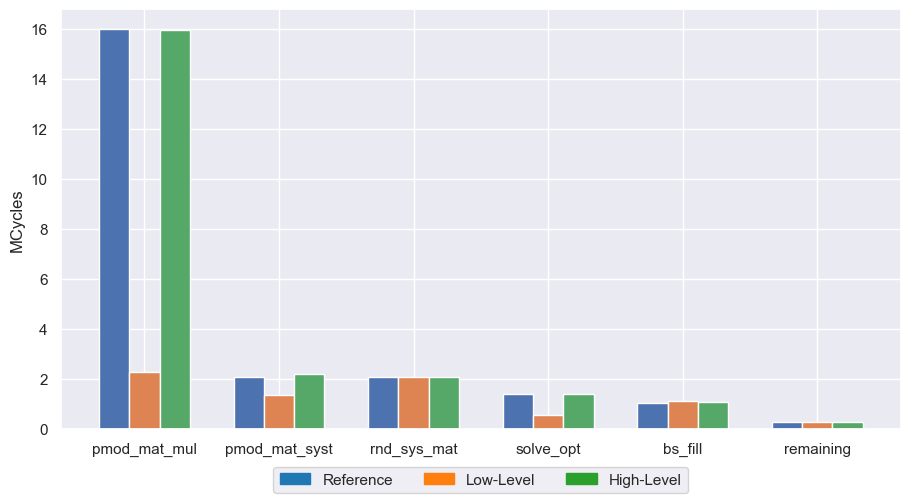
\includegraphics[width=\textwidth]{plots/barplot_MEDS-55520_profile_keygen.png}
  \caption{MEDS-55520 profiling results for functions used in key generation.}
  \label{fig:results_profile_keygen_MEDS-55520}
\end{figure}

\begin{figure}
  \centering
  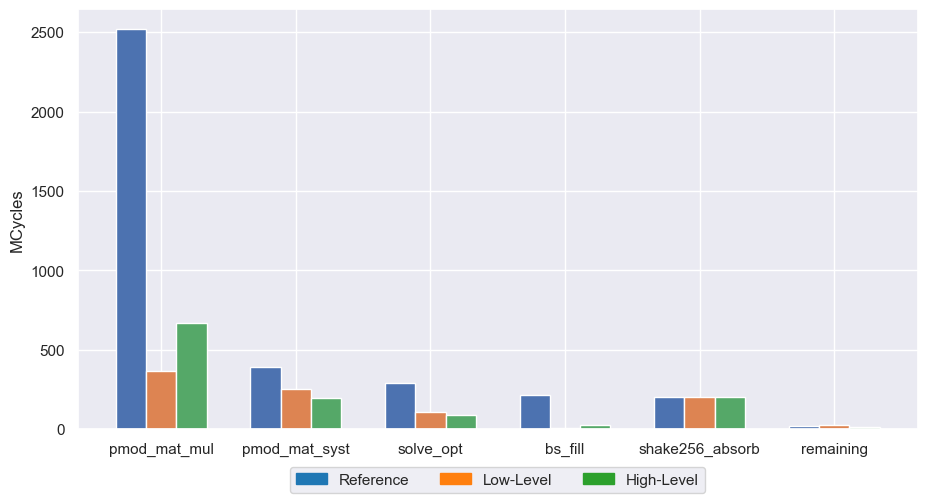
\includegraphics[width=\textwidth]{plots/barplot_MEDS-55520_profile_sign.png}
  \caption{MEDS-55520 profiling results for functions used in signing.}
  \label{fig:results_profile_signing_MEDS-55520}
\end{figure}

\begin{figure}
  \centering
  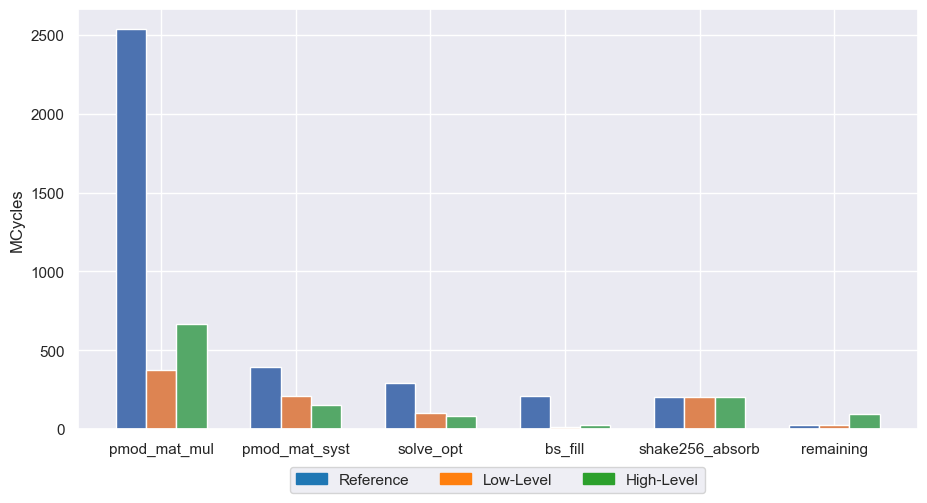
\includegraphics[width=\textwidth]{plots/barplot_MEDS-55520_profile_verify.png}
  \caption{MEDS-55520 profiling results for functions used in verification.}
  \label{fig:results_profile_verify_MEDS-55520}
\end{figure}

The figures show major improvements for all three algorithms in both the low-level and high-level optimized implementations, with a few notable exceptions:
\begin{itemize}
  \item The key generation algorithm used in the high-level optimized implementation is the same as the one in the reference implementation, because the parameter sets that we consider do not allow for large speedup factors for the high-level optimizations of this algorithm. We leave this as future work (see Section~\ref{sec:futureworkopt}).
        \pagebreak
  \item In key generation, the \texttt{rnd\_sys\_mat} (responsible for generating random systemized matrices) and \texttt{bs\_fill} (responsible for writing to a bitstream) functions have not been optimized, and therefore show no improvement. Generating random systemized matrices cannot be optimized, as it relies on the generation of random field elements using the SHAKE256 XOF (which is already optimized). Writing to a bitstream can be optimized using the approach described in Section~\ref{sec:bitstreamfilling}, which we leave as future work.
  \item The \texttt{shake256\_absorb} function used in signing and verification does not show any improvement. This is because the SHAKE256 XOF is already heavily optimized. The only thing that can be optimized is the structure of the hashing process, which we execute and explain in Section~\ref{sec:hashfunctionoptimization}.
\end{itemize}

Besides these exceptions, the results show that the optimizations have been very effective. Particularly matrix multiplication shows a huge speedup, but the other functions also show major improvements. We note the following observations:
\begin{itemize}
  \item The low-level optimized matrix multiplication function is faster than its high-level optimized counterpart. We believe that this is because the high-level optimized function needs to access 8 times as many values in memory as the low-level optimized function. This results in a larger amount of cache misses, which slows down the function.
  \item The high-level optimized matrix systemizer function is faster than its low-level optimized counterpart. We believe that this is because the low-level optimized function is not able to parallelize every aspect of the systemizer process (such as the inversion of field elements), whereas the high-level optimized function can do this. This results in a larger speedup for the high-level optimized function.
  \item The high-level optimized isometry derivation function is slightly faster than its low-level optimized counterpart. We believe that this is because the high-level optimized function parallelizes the entire function, whereas the low-level optimized function only parallelizes the two most time-consuming loops. The low-level optimized function might therefore benefit from further optimization, which we leave as future work (see Section~\ref{sec:futureworkopt}).
\end{itemize}

\section{Overall performance}
\label{sec:overallperformance}
We have benchmarked the performance of the MEDS for all combinations of the three relevant variables to consider:
\begin{itemize}
  \item \textbf{MEDS parameter set}: We analyzed the performance for each of the three considered parameter sets: MEDS-21595, MEDS-55520, and MEDS-122000 (see Section~\ref{sec:parametersets}).
  \item \textbf{Algorithm}: We tested each of the three signature algorithms: key generation, signing, and verification.
  \item \textbf{Implementation variant}: We tested all implementations: reference, low-level optimized, high-level optimized, low-level optimized with alternative hash structure, and high-level optimized with alternative hash structure.
\end{itemize}
MEDS was benchmarked for every possible combination of these variables, resulting in a total of 45 benchmarks. The result for each benchmark was obtained in the following way:
\begin{enumerate}
  \item 16 `warmup' runs were executed to ensure that the cache was filled with the necessary data and the branch predictor was optimized;
  \item 128 measurement runs were executed to obtain 128 measurements of the execution time of the algorithm;
  \item The final benchmark result was obtained by taking the median of the 128 measurements.
\end{enumerate}

The exact results of the benchmarks are shown in Table~\ref{tab:overall_benchmark_results_21595} (MEDS-21595), Table~\ref{tab:overall_benchmark_results_55520} (MEDS-55520), and Table~\ref{tab:overall_benchmark_results_122000} (MEDS-122000) in Appendix~\ref{app:benchmark_results}. As the relative performance of the implementations is more important than the exact numbers, we depict the results in the form of bar charts in Figure~\ref{fig:overal_performance_bar_chart_MEDS-21595} (MEDS-21595), Figure~\ref{fig:overal_performance_bar_chart_MEDS-55520} (MEDS-55520), and Figure~\ref{fig:overal_performance_bar_chart_MEDS-122000} (MEDS-122000).

\begin{figure}
  \centering
  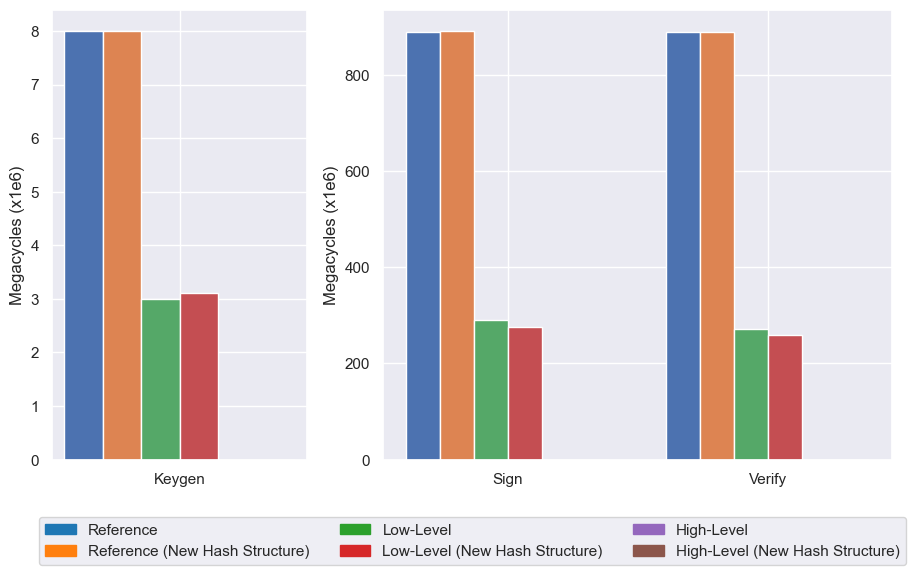
\includegraphics[width=\textwidth]{plots/barplot_MEDS-21595.png}
  \caption{Overall performance of MEDS-21595 variants. Low-Level refers to the low-level optimized implementation and High-Level to the high-level optimized implementation. The `New Hash Structure' variants refer to the optimized hash structure described in Section~\ref{sec:hashfunctionoptimization}.}
  \label{fig:overal_performance_bar_chart_MEDS-21595}
\end{figure}

\begin{figure}
  \centering
  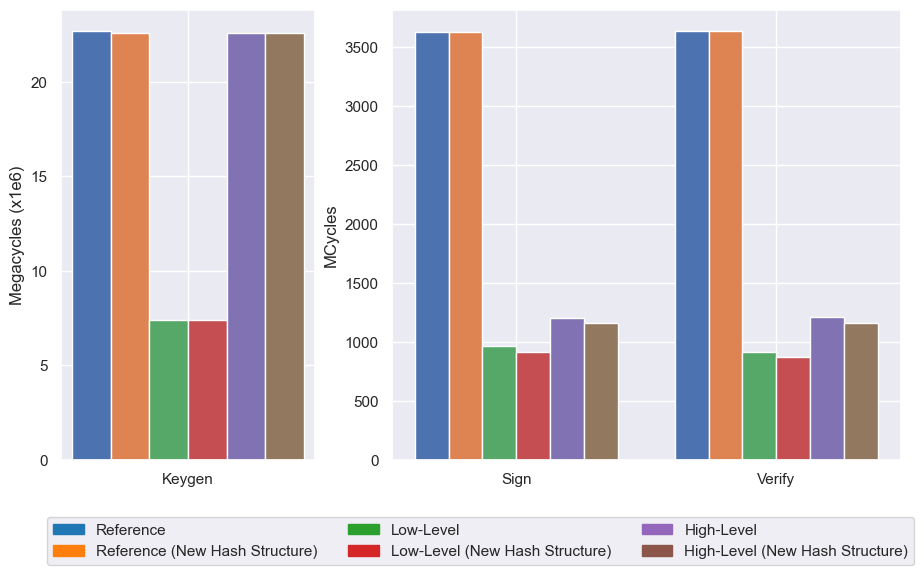
\includegraphics[width=\textwidth]{plots/barplot_MEDS-55520.png}
  \caption{Overall performance of MEDS-55520 variants. Low-Level refers to the low-level optimized implementation and High-Level to the high-level optimized implementation. The `New Hash Structure' variants refer to the optimized hash structure described in Section~\ref{sec:hashfunctionoptimization}.}
  \label{fig:overal_performance_bar_chart_MEDS-55520}
\end{figure}

\begin{figure}
  \centering
  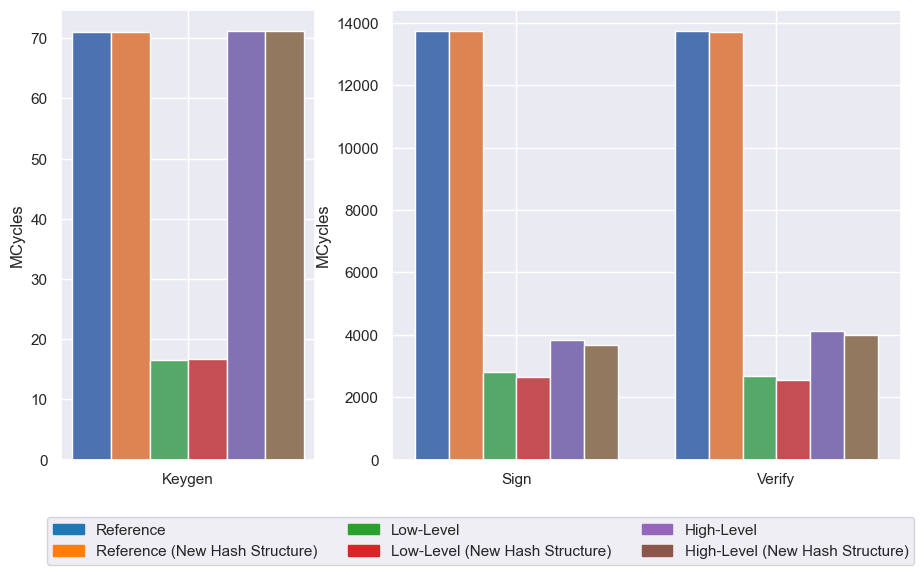
\includegraphics[width=\textwidth]{plots/barplot_MEDS-122000.png}
  \caption{Overall performance of MEDS-122000 variants. Low-Level refers to the low-level optimized implementation and High-Level to the high-level optimized implementation. The `New Hash Structure' variants refer to the optimized hash structure described in Section~\ref{sec:hashfunctionoptimization}.}
  \label{fig:overal_performance_bar_chart_MEDS-122000}
\end{figure}

The results show that both the low-level and high-level optimizations have resulted in a major speedup of the MEDS implementation (except for high-level key generation). The low-level optimized implementation is faster than the high-level optimized implementation for all algorithms and parameter sets. This is because the high-level optimized variant needs to transfer larger amounts of data to and from the various functions it uses, causing a larger amount of cache misses, which slows down the implementation.

Additionally, the results show that the alternative hash structure presented in Section~\ref{sec:hashfunctionoptimization} results in a small speedup for the signing and verification algorithms. It does not have a noticeable impact when applied to the reference implementation.

\section{Comparison to similar schemes}
\label{sec:comparison}
We compare the performance of MEDS to the performance of other digital signature schemes. Note that we compare to the self-reported performance of the schemes over various CPUs, which means the results are not directly comparable. Nevertheless, the comparison indicates the rough relative performance of the schemes. Besides this, note that the comparison is only based on the performance of the schemes and does not take key and signature sizes into account.

For reference, we include a comparison to Dilithium~\cite{ducas2018crystals}, Falcon~\cite{fouque2018falcon}, and SPHINCS$^+$~\cite{aumasson2022sphincs}, the three selected signature schemes in the initial NIST post-quantum standardization process. More importantly though, we compare to a set of related (mostly code-based) post-quantum digital signature schemes that are, like MEDS, in the current NIST post-quantum digital signature standardization process. The results are shown in Table~\ref{tab:codebasedcomparison}.

% \begin{table}
%   \centering
%   \caption{Comparison of MEDS performance to self-reported times of standardized post-quantum digital signature schemes that have been optimized for ARMv8. The numbers represent the number of KCycles that the key generation, signing, and verification algorithms take to execute on an ARM Cortex-A72 CPU.}
%   \begin{tabular}{p{1.1cm}lrrr}
%     \toprule
%     \textbf{NIST Level}  & \textbf{Work}                    & \textbf{Keygen} & \textbf{Sign} & \textbf{Verify} \\
%     \midrule
%     \multirow{3}{*}{I}   & Falcon512~\cite{nguyen2023fast}  & -               & 1044.6        & 59.9            \\
%                          & Dilithium2~\cite{becker2021neon} & 269.7           & 649.2         & 272.8           \\
%                          & MEDS-21595 (ours)                & 2821.4          & 248223.4      & 229793.6        \\
%     \midrule
%     \multirow{2}{*}{III} & Dilithium3~\cite{becker2021neon} & 515.8           & 1089.4        & 447.5           \\
%                          & MEDS-55520 (ours)                & 7184.6          & 927910.3      & 878268.2        \\
%     \midrule
%     \multirow{3}{*}{V}   & Falcon1024~\cite{nguyen2023fast} & -               & 2137.0        & 125.2           \\
%                          & Dilithium5~\cite{becker2021neon} & 782.8           & 1437.0        & 764.9           \\
%                          & MEDS-122000 (ours)               & 16646.2         & 2794525.4     & 2693826.8       \\
%     \bottomrule
%   \end{tabular}
%   \label{tab:stdcomparison}
% \end{table}

\begin{table}
  \centering
  \caption{Comparison of MEDS performance to self-reported times of other similar or relevant signature schemes in the NIST standardization process. The numbers represent the number of MCycles that the key generation, signing, and verification algorithms take on the mentioned CPUs: (1)~AMD~Ryzen~5~Pro~3500U, (2)~Intel~Core~i7-12700, (3)~Intel~Comet~Lake, (4)~ARM~Cortex-A72, (5)~Intel~i5-1135G7, (6)~Intel~Xeon~E-25588G, (7)~Intel~Xeon~E3-1220, (8)~Intel~Core~i9-13900K. For SPHINCS$^+$ measurements, the SHA2-simple variant is used.\\}
  \resizebox{\textwidth}{!}{
    %
    \begin{tabular}{p{1.1cm}lrrrr}
      \toprule
      \textbf{NIST Level} & \textbf{Scheme}                                    & \textbf{CPU} & \textbf{Keygen} & \textbf{Sign} & \textbf{Verify} \\
      \midrule
      \multirow{12}{*}{I}
                          & Dilithium2 (NEON)~\cite{becker2021neon}            & (4)          & 0.27            & 0.65          & 0.27            \\
                          & Falcon512 (NEON)~\cite{nguyen2023fast}             & (4)          & -               & 1.04          & 0.06            \\
                          & SPHINCS$^+$-128s (AVX2)~\cite{aumasson2022sphincs} & (7)          & 84.97           & 644.74        & 0.86            \\
      \addlinespace[0.5em]
                          & Balanced-ALTEQ~\cite{blaser2024alteq}              & (6)          & 0.36            & 2.74          & 2.11            \\
                          & CROSS-R-SDP-b~\cite{baldi2024cross}                & (1)          & 0.04            & 2.38          & 1.44            \\
                          & LESS-1b (AVX2)~\cite{baldi2024less}                & (2)          & 0.90            & 263.60        & 271.40          \\
                          & MEDS-21595 (reference)                             & (4)          & 7.97            & 890.71        & 889.77          \\
                          & MEDS-21595 (ours)                                  & (4)          & 2.82            & 248.22        & 229.79          \\
                          & PERK-I-short3 (AVX2)~\cite{aaraj2023perk}          & (8)          & 0.08            & 38.0          & 27.0            \\
                          & RYDE-128S (AVX2)~\cite{aragon2023ryde}             & (8)          & 0.03            & 23.40         & 20.10           \\
                          & uov-Ip-classic (NEON)~\cite{beullens2023uov}       & (4)          & 11.17           & 0.25          & 0.14            \\
                          & Wave822~\cite{banegas2023wave}                     & (5)          & 13946.20        & 1156.18       & 206.10          \\
      \midrule
      \multirow{11}{*}{III}
                          & Dilithium3 (NEON)~\cite{becker2021neon}            & (4)          & 0.52            & 1.09          & 0.45            \\
                          & SPHINCS$^+$-192s (AVX2)~\cite{aumasson2022sphincs} & (7)          & 125.31          & 1246.38       & 1.44            \\
      \addlinespace[0.5em]
      % \addlinespace[0.2em] \arrayrulecolor{gray} \cline{2-6} \arrayrulecolor{black} \addlinespace[0.2em]
                          & Balanced-ALTEQ~\cite{blaser2024alteq}              & (6)          & 2.23            & 28.46         & 26.20           \\
                          & CROSS-R-SDP-b~\cite{baldi2024cross}                & (1)          & 0.08            & 4.97          & 2.89            \\
                          & LESS-3b (AVX2)~\cite{baldi2024less}                & (2)          & 2.80            & 2446.90       & 2521.40         \\
                          & MEDS-55520 (reference)                             & (4)          & 22.66           & 3623.80       & 3628.16         \\
                          & MEDS-55520 (ours)                                  & (4)          & 7.18            & 927.91        & 878.27          \\
                          & PERK-III-short3 (AVX2)~\cite{aaraj2023perk}        & (8)          & 0.18            & 80.0          & 64.0            \\
                          & RYDE-192S (AVX2)~\cite{aragon2023ryde}             & (8)          & 0.05            & 49.60         & 44.80           \\
                          & uov-III-classic (NEON)~\cite{beullens2023uov}      & (4)          & 66.87           & 1.54          & 0.57            \\
                          & Wave1249~\cite{banegas2023wave}                    & (5)          & 46285.89        & 3534.75       & 467.36          \\
      \midrule
      \multirow{11}{*}{V}
                          & Dilithium5 (NEON)~\cite{becker2021neon}            & (4)          & 0.78            & 1.44          & 0.77            \\
                          & Falcon1024 (NEON)~\cite{nguyen2023fast}            & (4)          & -               & 2.14          & 0.13            \\
                          & SPHINCS$^+$-256s (AVX2)~\cite{aumasson2022sphincs} & (7)          & 80.94           & 1025.72       & 1.99            \\
      \addlinespace[0.5em]
      % \addlinespace[0.2em] \cline{2-6} \addlinespace[0.2em]
                          & CROSS-R-SDP-b~\cite{baldi2024cross}                & (1)          & 0.14            & 8.26          & 5.00            \\
                          & LESS-5b (AVX2)~\cite{baldi2024less}                & (2)          & 6.40            & 10212.60      & 10458.80        \\
                          & MEDS-122000 (reference)                            & (4)          & 71.02           & 13748.90      & 13731.38        \\
                          & MEDS-122000 (ours)                                 & (4)          & 16.65           & 2794.53       & 2693.83         \\
                          & PERK-V-short3 (AVX2)~\cite{aaraj2023perk}          & (8)          & 0.31            & 182.0         & 142.0           \\
                          & RYDE-256S (AVX2)~\cite{aragon2023ryde}             & (8)          & 0.07            & 105.50        & 95.90           \\
                          & uov-V-classic (NEON)~\cite{beullens2023uov}        & (4)          & 313.81          & 3.32          & 1.32            \\
                          & Wave1644~\cite{banegas2023wave}                    & (5)          & 106260.00       & 7851.48       & 806.86          \\
      \bottomrule
    \end{tabular}
    %
  }
  \label{tab:codebasedcomparison}
\end{table}

When comparing the performance of MEDS to other similar post-quantum digital signature schemes, the results are mixed. ALTEQ, CROSS, PERK, and RYDE outperform MEDS for all three algorithms. UOV also outperforms MEDS by a large factor, except for key generation. MEDS performs relatively similar to LESS, although for larger security levels, LESS is significantly slower at generating and verifying signatures. The only scheme that MEDS outperforms for all three algorithms is Wave. Although these results do not seem too promising, it is important to note that, except for Wave, MEDS provides smaller signature sizes than all of these schemes. This makes MEDS a viable competitor in the digital signature scheme landscape.

When comparing the performance of MEDS to standardized post-quantum digital signature schemes, we see that MEDS is significantly slower than Falcon and Dilithium but can compete with SPHINCS$^+$. Although MEDS and a lot of other schemes are slower than Falcon and Dilithium, they can still be viable alternatives. Firstly, there can be specialized use cases where performance is not the most important factor, and where the potentially smaller key or signature sizes of alternative schemes are more important. Secondly, standardizing schemes that rely on different mathematical problems provides more diversity in security assumptions. If the security of structured lattices (on which both Falcon and Dilithium rely) is ever broken, it is important to have alternative schemes that rely on different mathematical problems.

\pagebreak

\section{Discussion}
Throughout our research, we have found answers to our research questions.
\begin{itemize}[left=35pt,labelsep=15pt]
  \item[RQ I.] From our profiling efforts in Chapter~\ref{ch:profiling}, we have found that the matrix multiplication, the matrix systemizer, and isometry derivation functions are the most time-consuming functions in the MEDS implementation. Together, they account for over 87~\% of the total execution time of the MEDS implementation. After optimizing these functions, we have found that these functions still take up a significant amount of the total execution time. Additionally, we found that the KECCAK permutation now takes up a significant amount of time in all three algorithms.
  \item[RQ II.] We have found that the low-level optimization approach results in a large speedup for all parameter sets. The high-level optimization approach is less effective but still results in a significant speedup. On architectures with larger cache sizes and/or larger SIMD registers, the high-level optimization approach might be more effective. As for the low-level approach, we optimized the matrix multiplication, matrix systemizer, and isometry derivation functions using NEON instructions. Additionally, we obtained a speedup by optimizing the bitstream filling process and suggested a new hash structure that allows for parallelization of the hashing process, providing another small speedup.
        \begin{itemize}
          \item[a)] The bitstream filling and hash restructure speedups can be applied to the reference implementation as they do not require any ARMv8-specific instructions. The remaining optimizations (which make up the bulk of the speedup) are ARMv8-specific and can therefore not directly be applied to the reference implementation. However, most other architectures have their own SIMD instruction set, which can be used in the same way as NEON instructions and should achieve similar speedups.
        \end{itemize}
\end{itemize}

\chapter{Conclusions}
\label{ch:conclusion}
From the results in Chapter~\ref{ch:results}, it is clear that our optimizations have resulted in a major speedup of the MEDS implementation. The low-level optimization approach (as described in Section~\ref{sec:lowleveloptimization}) has provided the highest speedup, with MEDS-21595 being sped up by a factor of 2.9, 3.6, and 3.9 for key generation, signing, and verification, respectively; MEDS-55520 by factors 3.2, 3.9, and 4.1; and MEDS-122000 by factors 4.3, 4.9, and 5.1. The high-level optimization approach (as described in Section~\ref{sec:highleveloptimization}) has provided a smaller speedup due to the limitations in the cache size of the ARM Cortex-A72 CPU. This approach might provide a larger speedup on CPUs with larger cache sizes.

We present an alternative hash structure in Section~\ref{sec:hashfunctionoptimization} that improves the performance of signing and verification by a small amount, at a negligible cost to the non-parallelized reference implementation. Since MEDS produces different challenges and signatures when using this alternative hash structure, we leave it as a suggested change to the MEDS scheme.

We have shown that the MEDS implementation is very suitable for optimization using SIMD instructions. The achieved speedup on ARMv8 is big, but we expect that future research can achieve even larger speedups on other architectures that support SIMD instructions, such as AVX512~\cite{intel-avx512}, on which 4 times as many field elements can be processed in parallel compared to ARMv8.

Compared to standardized post-quantum signature schemes, MEDS is heavily outperformed by Falcon and Dilithium. However, if the security of structured lattices (on which both Falcon and Dilithium rely) is ever broken, MEDS can serve as a viable alternative, as it is based on a different mathematical problem. When compared to other similar (code-based) post-quantum signature schemes, MEDS provides a smaller signature size than nearly all of them, but is outperformed by most of them in terms of performance. The choice between these schemes should be based on a wide range of factors, among which are the security requirements of the application, the performance requirements of the key generation, signing, and verification algorithms, the private and public key sizes, and the signature size.

\chapter{Future Work}
\label{ch:futurework}
Although we have optimized the MEDS implementation significantly, we have mentioned several limitations and possible improvements. In this chapter, we discuss these ideas in more detail. Additionally, there are some other unexplored but interesting topics that we discuss.

\section{Further optimization possibilities}
\label{sec:futureworkopt}

\subsection*{Bitstream optimization}
As explained in Section~\ref{sec:bitstreamfilling}, the commitment matrices are hashed by first converting them into a bitstream. An alternative approach is to change the pointer type of the matrix elements from 16-bit to 8-bit unsigned integers (which would practically take no time to execute) and then hash the resulting array. The main advantage of this approach is that we no longer need to execute the relatively costly bitstream filling process. However, it also comes at the cost of having $\frac{4}{3}$ times as many values to hash. It would be interesting to see if this approach results in a speedup of the general hashing process.

\subsection*{Optimizing isometry derivation}
Our optimizations to the isometry derivation function \texttt{solve\_opt} as described in Section~\ref{sec:isometryderivation} have been very effective, resulting in a speedup factor of 2.7 for MEDS-55520 (see also the results in Section~\ref{sec:profilingoptimizations}). However, our optimizations were solely based on the vectorization of the two most time-consuming loops in the \texttt{solve\_opt} function using NEON intrinsics. We expect that an additional speedup can be achieved by optimizing the remaining loops in the function. Additionally, we believe that a pure-assembly approach will result in an even larger speedup.

\subsection*{Additional multiplication techniques for specific matrix dimensions}
We have heavily optimized the matrix multiplication function, achieving an average matrix multiplication speedup factor of 6.9 for MEDS-55520 (see also the results in Section~\ref{sec:profilingoptimizations}). Naturally, the optimizations are slightly less effective for matrices that use dimensions that are not a multiple of 8. For most matrix sizes, the results were still close to the lower bound. However, we noticed that matrices with dimensions $2 \times x$ were not optimized as well as we would have liked. The creation of an additional algorithm that is specifically tailored to such matrix sizes could pull the performance of these matrix multiplications closer to the lower bound.

\subsection*{High-level key generation optimization}
We have not applied high-level optimizations to the key generation function. The main loop of the key generation generates all $s$ matrices that represent the public key. For the parameter sets that we consider, $s$ is always 2, which heavily limits the possibilities for parallelization. The speedup factor would be limited to 2, which we already exceeded with our low-level optimizations. However, it might still be interesting to explore the possibilities for high-level optimizations for key generation, especially considering that the need for parameter sets with larger values of $s$ might arise in the future.

\section{Additional research topics}
\label{sec:futureworkresearch}

\subsection*{Memory and power usage analysis}
We have focused on optimizing the performance of the MEDS implementation, but we have not analyzed the memory and power usage of any of the implementations. It would be interesting to see what the impact of our optimizations on memory and power usage is. Additionally, the possibilities for further optimizations in these areas could be explored, which is especially relevant for embedded systems and IoT devices.

\subsection*{Optimizing for other CPU architectures}
We have optimized the MEDS implementation for the ARMv8 architecture, but many other CPU architectures support SIMD instructions. One interesting architecture to explore is the AVX512 architecture, which is supported by Intel and AMD CPUs. AVX512 can process 4 times as many field elements in parallel compared to ARMv8, which could result in a significant speedup of the MEDS implementation.

\bibliographystyle{plain}
\bibliography{bibliofile}

\appendix
\chapter{MEDS Algorithms}
\label{app:medsalgs}

\section{Notations and Functions}

\subsection{Notations}
In the algorithms in this appendix, we use the following notations in addition to the notations mentioned in Section \ref{sec:notations}:
\begin{itemize}
  \item $\ell_{x}$: The size of the variable $x$ in bytes.
  \item $\mathcal{B}^{x}$: The set of all byte strings of length $x$.
  \item $\sigma$: A seed used to generate random values.
  \item $\text{GL}_k(q)$: The set of all invertible $k \times k$ matrices over $\mathds{F}_q$.
  \item $b[i,j]$: The $j-i$ byte long substring of byte string $b$ starting at index $i$.
  \item $\textbf{A}[;i,j]$: The submatrix of $\textbf{A}$ that starts at column $i$ (inclusive) and ends at column $j$ (exclusive), containing all rows.
  \item $(x~|~y)$: The concatenation of byte strings $x$ and $y$.
\end{itemize}

\subsection{Functions}
In the algorithms in this appendix, we use the following functions (in order of appearance):
\begin{itemize}
  \item Randombytes($x$): Generates a random byte string of length $x$.
  \item ExpandSysMat($\sigma$): Generate a random systematic matrix from seed $\sigma$.
  \item XOF($\sigma$, $x$, $y$): Generates two random byte strings of length $x$ and $y$ from seed $\sigma$.
  \item ExpandInvMat($\sigma$, $k$): Generates a random invertible matrix of size $k \times k$ from seed $\sigma$.
  \item Solve($\textbf{G}$): Solves the system of linear equations represented by matrix $\textbf{G}$.
  \item SF($\textbf{G}$): Converts matrix $\textbf{G}$ to systematic form.
  \item Compress(G)($\textbf{A}$): Compresses matrix $\textbf{A}$ into a byte string.
  \item Decompress(G)($x$): Decompresses byte string $x$ into a matrix.
  \item SeedTree$_t(\rho, \alpha)$: Constructs a seed tree of height $\log_2(t)$ from root seed $\rho$ and salt $\alpha$ and return the first $t$ leaf nodes.
  \item ToBytes($x$, $y$): Converts $x$ to a byte string of length $y$.
  \item ExpandRndMat($\sigma$): Generates a random matrix from seed $\sigma$.
  \item H($x$): Hashes byte string $x$.
  \item ParseHash$_{s,t,w}(d)$: Parses hash $d$ into $t$ challenges that are smaller than $s$ each, where $w$ challenges are 0.
  \item SeedTreeToPath$_t(h_0, \ldots, h_{t-1}, \rho, \alpha)$: Reconstructs a seed tree with the same structure as SeedTree$_t(\rho, \alpha)$. Based on the values of $h_0, \ldots, h_{t-1}$, returns a seed-tree path with which the leaf node seeds can be reconstructed.
  \item ParseSig($m_s$): Parses the signed message $m_s$ into its components.
  \item PathToSeedTree$_t(h_0, \ldots, h_{t-1}, p, \alpha)$: Reconstructs a seed tree with the same structure as SeedTree$_t(\rho, \alpha)$. Based on the values of $h_0, \ldots, h_{t-1}$ and the path $p$, returns the seeds of the leaf nodes.
\end{itemize}

\section{Main Algorithms}
\begin{algorithm}[H]
\caption{MEDS.KeyGen()}\label{alg:medskeygen}
\hspace*{\algorithmicindent} \textbf{Input:} -\\
\hspace*{\algorithmicindent} \textbf{Output:} public key $\textbf{pk} \in \mathcal{B}^{\ell_\textbf{pk}}$, secret key $\textbf{sk} \in \mathcal{B}^{\ell_\textbf{sk}}$
\begin{algorithmic}[1]
% Generate a random secret seed
\State $\delta \in \mathcal{B}^{\ell_\text{sec\_seed}} \gets \text{Randombytes}(\ell_\text{sec\_seed})$
% Generate random secret and public seed from the previously generated secret seed
\State $\sigma_{\textbf{G}_0} \in \mathcal{B}^{\ell_\text{pub\_seed}}, \sigma \in \mathcal{B}^{\ell_\text{sec\_seed}} \gets \text{XOF}(\delta, \ell_\text{pub\_seed}, \ell_\text{sec\_seed})$
% Generate a random matrix G_0 from the public seed
\State $\textbf{G}_0 \in \mathds{F}_q^{k \times mn} \gets \text{ExpandSysMat}(\sigma_{\textbf{G}_0})$
% Generate G_i for every s
\ForAll{$i \in \{1, \ldots, s - 1\}$}
    % Generate two new seeds from the current state of the secret seed and replace the current secret seed
    \State $\sigma_{\textbf{T}_i}, \sigma \in \mathcal{B}^{\ell_\text{sec\_seed}} \gets \text{XOF}(\sigma, \ell_\text{sec\_seed}, \ell_\text{sec\_seed})$
    % Generate a random invertible matrix T_i
    \State $\textbf{T}_i \in \text{GL}_k(q) \gets \text{ExpandInvMat}(\sigma_{\textbf{T}_i}, k)$
    % Compute G_0' = T_i * G_0
    \State $\textbf{G}_0' \in \mathds{F}_q^{k \times mn} \gets \textbf{T}_i \textbf{G}_0$
    % Solve system of equations to obtain A and B
    \State $\check{\textbf{A}}_i \in \mathds{F}_q^{m \times m} \cup \{\bot\}, \check{\textbf{B}}_i \in \mathds{F}_q^{n \times n} \cup \{\bot\} \gets \text{Solve}(\textbf{G}_0')$
    % Retry if there was no solution
    \If{$(\check{\textbf{A}}_i = \bot \textbf{ and } \check{\textbf{B}}_i = \bot) \textbf{ or } \check{\textbf{A}}_i \notin \text{GL}_m(q) \textbf{ or } \check{\textbf{B}}_i \notin \text{GL}_n(q)$}
        \State \textbf{goto} line 5
    \EndIf
    % Get A_i, A_i^-1, B_i, and B_i^-1 from the solution
    % Theoretically we don't need to rename these variables, but it is done for notation
    \State $\textbf{A}_i, \textbf{A}_i^{-1} \in \text{GL}_m(q) \gets \check{\textbf{A}}_i, \check{\textbf{A}}_i^{-1}$
    \State $\textbf{B}_i, \textbf{B}_i^{-1} \in \text{GL}_n(q) \gets \check{\textbf{B}}_i, \check{\textbf{B}}_i^{-1}$
    % Compute Gi
    \State $\textbf{G}_i \in \mathds{F}_q^{k \times mn} \gets \pi_{\textbf{A}_i, \textbf{B}_i}(\textbf{G}_0)$
    % Compute Compute T_i^-1 as a k*k submatrix of G_i
    \State $\textbf{T}_i^{-1} \in \mathds{F}_q^{k \times k} \gets \textbf{G}_i[;0,k-1]$
    % Convert Gi to systematic form
    \State $\textbf{G}_i \in \mathds{F}_q^{k \times mn} \cup \{\bot\} \gets \text{SF}(\textbf{G}_i)$
    % Retry if the matrix is not in systematic form
    \If{$\textbf{G}_i = \bot$}
        \State \textbf{goto} line 5
    \EndIf
    \EndFor
% Compute the pk from the data
\State $\text{pk} \in \mathcal{B}^{\ell_\textbf{pk}} \gets (\sigma_{\textbf{G}_0}~|~\text{CompressG}(\textbf{G}_1)~|~\ldots~|~\text{CompressG}(\textbf{G}_{s-1}))$
% Compute the sk from the data
\State $\text{sk} \in \mathcal{B}^{\ell_\textbf{sk}} \gets (\delta~|~\sigma_{\textbf{G}_0}~|~\text{Compress}(\textbf{A}_1^{-1})~|~\ldots~|~\text{Compress}(\textbf{A}_{s-1}^{-1})$\\
$\quad\quad\quad\quad\quad\quad\quad\quad\quad~|~\text{Compress}(\textbf{B}_1^{-1})~|~\ldots~|~\text{Compress}(\textbf{B}_{s-1}^{-1})$\\
$\quad\quad\quad\quad\quad\quad\quad\quad\quad~|~\text{Compress}(\textbf{T}_1^{-1})~|~\ldots~|~\text{Compress}(\textbf{T}_{s-1}^{-1}))$
% Return the public and secret key
\State \textbf{return} $\text{pk}, \text{sk}$
\end{algorithmic}
\end{algorithm}

\newpage

\begin{algorithm}[H]
\caption{MEDS.Sign()}\label{alg:medssign}
\hspace*{\algorithmicindent} \textbf{Input:} secret key $\textbf{sk} \in \mathcal{B}^{\ell_\textbf{sk}}$, message $m \in \mathcal{B}^{\ell_m}$\\
\hspace*{\algorithmicindent} \textbf{Output:} signed message $m_s \in \mathcal{B}^{\ell_\text{sig} + \ell_m}$
\begin{algorithmic}[1]
% Initialize parsing index
\State $f_\text{sk} \gets \ell_\text{sec\_seed}$
% Parse sigma_G_0 from the secret key
\State $\sigma_{\textbf{G}_0} \gets \text{pk}[f_\text{sk}, f_\text{sk} + \ell_\text{pub\_seed} - 1]$
% Construct G0
\State $\textbf{G}_0 \in \mathds{F}_q^{k \times mn} \gets \text{ExpandSysMat}(\sigma_{\textbf{G}_0})$
% Increment index; skip public seed and A and B?
\State $f_\text{sk} \gets f_\text{sk} + \ell_\text{pub\_seed} + (s - 1) \cdot (\ell_{\mathds{F}_q^{m \times m}} + \ell_{\mathds{F}_q^{n \times n}})$
% % Obtain all A_i from the secret key
% \ForAll{$i \in \{1, \ldots, s - 1\}$}
%     % Parse A_i from the secret key
%     \State $\textbf{A}_i^{-1} \in \mathds{F}_q^{m \times m} \gets \text{Decompress}(\text{sk}[f_\text{sk}, f_\text{sk} + \ell_{\mathds{F}_q^{m \times m}}])$
%     % Update the parsing index
%     \State $f_\text{sk} \gets f_\text{sk} + \ell_{\mathds{F}_q^{m \times m}}$
% \EndFor
% % Obtain all B_i from the secret key
% \ForAll{$i \in \{1, \ldots, s - 1\}$}
%     % Parse B_i from the secret key
%     \State $\textbf{B}_i^{-1} \in \mathds{F}_q^{n \times n} \gets \text{Decompress}(\text{sk}[f_\text{sk}, f_\text{sk} + \ell_{\mathds{F}_q^{n \times n}}])$
%     % Update the parsing index
%     \State $f_\text{sk} \gets f_\text{sk} + \ell_{\mathds{F}_q^{n \times n}}$
% \EndFor
% Obtain all T_i from the secret key
\ForAll{$i \in \{1, \ldots, s - 1\}$}
    % Parse T_i from the secret key
    \State $\textbf{T}_i^{-1} \in \mathds{F}_q^{k \times k} \gets \text{Decompress}(\text{sk}[f_\text{sk}, f_\text{sk} + \ell_{\mathds{F}_q^{k \times k}}])$
    % Update the parsing index
    \State $f_\text{sk} \gets f_\text{sk} + \ell_{\mathds{F}_q^{k \times k}}$
\EndFor
% Generate a random seed
\State $\delta \in \mathcal{B}^{\ell_\text{sec\_seed}} \gets \text{Randombytes}(\ell_\text{sec\_seed})$
% Generate a random tree seed and salt from the secret seed
\State $\rho \in \mathcal{B}^{\ell_\text{tree\_seed}}, \alpha \in \mathcal{B}^{\ell_\text{salt}} \gets \text{XOF}(\delta, \ell_\text{tree\_seed}, \ell_\text{salt})$
% Construct t commitment seeds from the tree seed
\State $\sigma_0, \ldots, \sigma_{t-1} \in \mathcal{B}^{\ell_\text{tree\_seed}} \gets \text{SeedTree}_t(\rho, \alpha)$
% Generate t commitments from the challenge seeds
\ForAll{$i \in \{0, \ldots, t - 1\}$}
    % Construct a commitment seed for the current commitment
    \State $\sigma'_i \in \mathcal{B}^{\ell_\text{salt} + \ell_\text{tree\_seed} + 4} \gets (\alpha~|~\sigma_i~|~\text{ToBytes}(2^{1 + \lceil \log_2(t) \rceil + i}, 4))$
    % Generate seeds based on the current commitment seed
    \State $\sigma_{\tilde{\textbf{M}}_i} \in \mathcal{B}^{\ell_\text{pub\_seed}}, \sigma_i \in \mathcal{B}^{\ell_\text{tree\_seed}} \gets \text{XOF}(\sigma'_i, \ell_\text{pub\_seed}, \ell_\text{tree\_seed})$
    % Generate matrix ~M_i <- c0 and c1 represent the linear combination of codewords
    \State $\tilde{\textbf{M}}_i \in \mathds{F}_q^{2 \times k} \gets \text{ExpandRndMat}(\sigma_{\tilde{\textbf{M}}_i})$
    % Compute C = ~M_i * G_0 <- C contains the two codewords C0 and C1
    \State $\textbf{C} \in \mathds{F}_q^{2 \times mn} \gets \tilde{\textbf{M}}_i \textbf{G}_0$
    % Solve the system of equations to obtain A and B
    \State $\widetilde{\textbf{A}}_i \in \mathds{F}_q^{m \times m} \cup \{\bot\}, \widetilde{\textbf{B}}_i \in \mathds{F}_q^{n \times n} \cup \{\bot\} \gets \text{Solve}(\textbf{C})$
    % Retry if there was no solution
    \If{$(\widetilde{\textbf{A}}_i = \bot \textbf{ and } \widetilde{\textbf{B}}_i = \bot) \textbf{ or } \widetilde{\textbf{A}}_i \notin \text{GL}_m(q) \textbf{ or } \widetilde{\textbf{B}}_i \notin \text{GL}_n(q)$}
        \State \textbf{goto} line 12 % 18?
    \EndIf
    % Compute G_i
    \State $\tilde{\textbf{G}}_i \in \mathds{F}_q^{k \times mn} \gets \pi_{\widetilde{\textbf{A}}_i, \widetilde{\textbf{B}}_i}(\textbf{G}_0)$
    % Convert G_i to systematic form
    \State $\tilde{\textbf{G}}_i \in \mathds{F}_q^{k \times mn} \cup \{\bot\} \gets \text{SF}(\tilde{\textbf{G}}_i)$
    % Retry if the matrix is not in systematic form
    \If{$\tilde{\textbf{G}}_i = \bot$}
        \State \textbf{goto} line 12 % 18?
    \EndIf
\EndFor
% Create hash
\State $d \in \mathcal{B}^{\ell_\text{digest}} \gets \text{H}(\text{Compress}(\tilde{\textbf{G}}_0[;k,mn-1])~|~\ldots$\\
$\quad\quad\quad\quad\quad\quad~~|~\text{Compress}(\tilde{\textbf{G}}_{t-1}[;k,mn-1])~|~m)$
% Parse challenges from the hash
\State $h_0, \ldots, h_{t-1} \in \{0, \ldots, s-1\} \gets \text{ParseHash}_{s,t,w}(d)$
% For each challenge, compute the response
\ForAll{$i \in \{0, \ldots, t - 1\}$}
    % Only for non-zero challenges
    \If{$h_i > 0$}
        % Compute response
        \State $\kappa_i \in \mathds{F}_q^{2 \times k} \gets \tilde{\textbf{M}}_i T_{h_i}^{-1}$
    \EndIf
\EndFor
% Construct seed tree paths
\State $p \in \mathcal{B}^{\ell_\text{path}} \gets \text{SeedTreeToPath}_t(h_0, \ldots, h_{t-1}, \rho, \alpha)$
% Return the signature
\State \textbf{return} $m_s \in \mathcal{B}^{w \cdot \ell_{\mathds{F}_q^{2 \times k}} + \ell_\text{path} + \ell_\text{digest} + \ell_\text{salt} + \ell_\text{m} = \ell_\text{sig} + \ell_\text{m}}$\\
$\quad\quad\quad\quad= (\kappa_0~|~\ldots~|~\kappa_{t-1}~|~p~|~d~|~\alpha~|~m)$
\end{algorithmic}
\end{algorithm}

\begin{algorithm}[H]
\caption{MEDS.Verify()}\label{alg:medsverify}
\hspace*{\algorithmicindent} \textbf{Input:} public key $\textbf{pk} \in \mathcal{B}^{\ell_\textbf{pk}}$, signed message $m_s \in \mathcal{B}^{\ell_\text{sig} + \ell_m}$\\
\hspace*{\algorithmicindent} \textbf{Output:} message $m \in \mathcal{B}^{\ell_m}$ or $\bot$
\begin{algorithmic}[1]
% Initialize parsing index
\State $\sigma_{\textbf{G}_0} \gets \text{pk}[0, \ell_\text{pub\_seed} - 1]$
% Construct G0
\State $\textbf{G}_0 \in \mathds{F}_q^{k \times mn} \gets \text{ExpandSysMat}(\sigma_{\textbf{G}_0})$
% Initialize parsing index
\State $f_\text{pk} \gets \ell_\text{pub\_seed}$
% Parse all G_i from the public key
\ForAll{$i \in \{1, \ldots, s - 1\}$}
    % Parse G_i from the public key
    \State $\textbf{G}_i \in \mathds{F}_q^{k \times mn} \gets \text{DecompressG}(\text{pk}[f_\text{pk}, f_\text{pk} + \ell_{\mathds{F}_q^{k \times mn}}])$
    % Update the parsing index
    \State $f_\text{pk} \gets f_\text{pk} + \ell_{G_i}$
\EndFor

% % Parse the path
% \State $p \in \mathcal{B}^{\ell_\text{path}} \gets m_s[\ell_\text{sig} - \ell_\text{digest} - \ell_\text{salt} - \ell_\text{path}, \ell_\text{sig} - \ell_\text{digest} - \ell_\text{salt} - 1]$
% % Parse the salt
% \State $\alpha \in \mathcal{B}^{\ell_\text{salt}} \gets m_s[\ell_\text{sig} - \ell_\text{digest} - \ell_\text{salt}, \ell_\text{sig} - \ell_\text{digest} - 1]$
% % Parse the digest
% \State $d \in \mathcal{B}^{\ell_\text{digest}} \gets m_s[\ell_\text{sig} - \ell_\text{digest}, \ell_\text{sig} - 1]$
% % Parse the message
% \State $m \in \mathcal{B}^{\ell_m} \gets m_s[\ell_\text{sig},]$
% % Compute the hash
% \State $h_0, \ldots, h_{t-1} \in \{0, \ldots, s-1\} \gets \text{ParseHash}_{s,t,w}(d)$

% Parse m_s
\State $p \in \mathcal{B}^{\ell_\text{path}}, \alpha \in \mathcal{B}^{\ell_\text{salt}}, d \in \mathcal{B}^{\ell_\text{digest}}, m \in \mathcal{B}^{\ell_m} \gets \text{ParseSig}(m_s)$
% Convert the path to seed tree seeds
\State $\sigma_0, \ldots, \sigma_{t-1} \in \mathcal{B}^{\ell_\text{tree\_seed}} \gets \text{PathToSeedTree}_t(h_0, \ldots, h_{t-1}, p, \alpha)$
% Loop through all t challenges
\ForAll{$i \in \{0, \ldots, t - 1\}$}
    \If{$h_i > 0$}
        % Non-zero challenges
        % Get kappa_i from the signature
        \State $\kappa_i \in \mathds{F}_q^{2 \times k} \gets m_s[i \cdot \ell_{\mathds{F}_q^{2 \times k}}, (i + 1) \cdot \ell_{\mathds{F}_q^{2 \times k}} - 1]$
        % Compute G0' = kappa * G[h_i]
        \State $\textbf{G}_0' \in \mathds{F}_q^{2 \times mn} \gets \kappa_i \textbf{G}_{h_i}$
        % Solve the system of equations to obtain A_hat and B_hat
        \State $\hat{\textbf{A}}_i \in \mathds{F}_q^{m \times m} \cup \{\bot\}, \hat{\textbf{B}}_i \in \mathds{F}_q^{n \times n} \cup \{\bot\} \gets \text{Solve}(\textbf{G}_0')$
        % Abort if there was no solution
        \If{$(\hat{\textbf{A}}_i = \bot \textbf{ and } \hat{\textbf{B}}_i = \bot) \textbf{or } \hat{\textbf{A}}_i \notin \text{GL}_m(q) \textbf{ or } \hat{\textbf{B}}_i \notin \text{GL}_n(q)$}
            \State \textbf{return} $\bot$
        \EndIf
        % Compute G_hat_i with pi
        \State $\hat{\textbf{G}}_i \in \mathds{F}_q^{k \times mn} \gets \pi_{\hat{\textbf{A}}_i, \hat{\textbf{B}}_i}(\textbf{G}_{h_i})$
        % Convert G_hat_i to systematic form
        \State $\hat{\textbf{G}}_i \in \mathds{F}_q^{k \times mn} \cup \{\bot\} \gets \text{SF}(\hat{\textbf{G}}_i)$
        % Abort if the matrix is not in systematic form
        \If{$\hat{\textbf{G}}_i = \bot$}
            \State \textbf{return} $\bot$
        \EndIf
    \Else
        % Zero challenges; we need to re-compute the G_i completely
        % Compute seed for the commitment
        \State $\sigma_i' \in \mathcal{B}^{\ell_\text{salt} + \ell_\text{tree\_seed} + 4} \gets (\alpha~|~\sigma_i~|~\text{ToBytes}(2^{1 + \lceil \log_2(t) \rceil + i}, 4))$
        % Generate seeds based on the current commitment seed
        \State $\sigma_{\hat{M}_i} \in \mathcal{B}^{\ell_\text{pub\_seed}}, \sigma_i \in \mathcal{B}^{\ell_\text{tree\_seed}} \gets \text{XOF}(\sigma_i', \ell_\text{pub\_seed}, \ell_\text{tree\_seed})$
        % Generate matrix M_hat_i <- c0 and c1 represent the linear combination of codewords
        \State $\hat{\textbf{M}}_i \in \mathds{F}_q^{2 \times k} \gets \text{ExpandRndMat}(\sigma_{\hat{\textbf{M}}_i})$
        % Compute C_hat_i = M_hat_i * G_0
        \State $\hat{\textbf{C}}_i \in \mathds{F}_q^{2 \times mn} \gets \hat{\textbf{M}}_i \textbf{G}_0$
        % Solve the system of equations to obtain A_hat and B_hat
        \State $\hat{\textbf{A}}_i \in \mathds{F}_q^{m \times m} \cup \{\bot\}, \hat{\textbf{B}}_i \in \mathds{F}_q^{n \times n} \cup \{\bot\} \gets \text{Solve}(\hat{\textbf{C}}_i)$
        % Retry if there was no solution
        \If{$(\hat{\textbf{A}}_i = \bot \textbf{ and } \hat{\textbf{B}}_i = \bot) \textbf{or } \hat{\textbf{A}}_i \notin \text{GL}_m(q) \textbf{ or } \hat{\text{B}}_i \notin \text{GL}_n(q)$}
            \State \textbf{goto} line 21
        \EndIf
        % Compute G_hat_i
        \State $\hat{\textbf{G}}_i \in \mathds{F}_q^{k \times mn} \gets \pi_{\hat{\textbf{A}}_i, \hat{\textbf{B}}_i}(\textbf{G}_0)$
        % Convert G_hat_i to systematic form
        \State $\hat{\textbf{G}}_i \in \mathds{F}_q^{k \times mn} \cup \{\bot\} \gets \text{SF}(\hat{\textbf{G}}_i)$
        % Retry if the matrix is not in systematic form
        \If{$\hat{\textbf{G}}_i = \bot$}
            \State \textbf{goto} line 21
        \EndIf
    \EndIf
\EndFor
% Compute the hash
\State $d' \in \mathcal{B}^{\ell_\text{digest}} \gets \text{H}(\text{Compress}(\hat{\textbf{G}}_0[;k,mn-1])~|~\ldots$\\
$\quad\quad\quad\quad\quad\quad~~|~\text{Compress}(\hat{\textbf{G}}_{t-1}[;k,mn-1])~|~m)$
% Verify the hash
\If{$d = d'$}
    \State \textbf{return} $m$
\Else
    \State \textbf{return} $\bot$
\EndIf
\end{algorithmic}
\end{algorithm}

\section{Supplemental Algorithms}
\label{app:supplementalalgs}
The MEDS key generation, signing, and verification algorithms require some additional algorithms to function. In this section, we present a few algorithms that are used by the three MEDS algorithms. Note that we do not list all supplemental algorithms, but only those that are relevant to our research.

\begin{algorithm}
  \caption{MEDS Matrix Multiplication}
  \label{alg:medsmatrixmultiplication}
  \begin{algorithmic}
    \Function{matrix\_mul}{$A \in \mathbb{F}_{4093}^{m \times n}, B \in \mathbb{F}_{4093}^{n \times o}$}
      \State $C \gets \text{zero matrix of size } m \times o$
      \For{$c \gets 0$ to $m$}
        \For{$r \gets 0$ to $o$}
          \For{$k \gets 0$ to $n$}
            \State $C[c][r] \gets C[c][r] + A[c][k] \cdot B[k][r]$
          \EndFor
          \State $C[c][r] \gets C[c][r] \mod 4093$
        \EndFor
      \EndFor
      \State \Return $C$
    \EndFunction
  \end{algorithmic}
\end{algorithm}

\begin{algorithm}
  \caption{MEDS `pi' function $\pi_{\textbf{A}, \textbf{B}}(\textbf{G})$}
  \label{alg:medspifunction}
  \begin{algorithmic}
    \Function{pi}{$\textbf{A} \in \mathbb{F}_{4093}^{m \times m}, \textbf{B} \in \mathbb{F}_{4093}^{n \times n}, \textbf{G} \in \mathbb{F}_{4093}^{k \times mn}$}
      \State $G' \gets \text{matrix (array) of size } k \times mn$
      \For{$i \gets 0$ to $k$}
        \State $G'[i \cdot mn, (i+1) \cdot mn] \gets \text{matrix\_mul}(\textbf{A}, \textbf{G}[i \cdot mn:(i+1) \cdot mn])$
        \State $G'[i \cdot mn, (i+1) \cdot mn] \gets \text{matrix\_mul}(\textbf{G}[i \cdot mn:(i+1) \cdot mn], \textbf{B})$
      \EndFor
      \State \Return $G'$
    \EndFunction
  \end{algorithmic}
\end{algorithm}

\begin{algorithm}
  \caption{MEDS Matrix Systemizer}
  \label{alg:systemizer}
  \begin{algorithmic}
    \Function{systemize}{$A \in \mathbb{F}_{4093}^{m \times n}$, $r_\text{max}$, do\_swap, do\_backsub}
      \State $ret \gets m \cdot \text{do\_swap}$
      \For{$r \gets 0$ to $r_\text{max}$}
        \State \texttt{// Attempt to make the diagonal element non-zero}
        \If{do\_swap}
          \State $z \gets 0$
          \For{$r_2 \gets r$ to $m$}
            \State $z \gets z$ or $A[r_2][r]$
          \EndFor
          \If{$z = 0$}
            \State $ret \gets r$
            \For{$i \gets 0$ to $r$}
              \State $A[i][r], A[i][n-1] \gets A[i][n-1], A[i][r]$
            \EndFor
          \EndIf
        \EndIf
        \For{$r_2 \gets r+1$ to $m$}
          \If{$A[r][r] = 0$}
            \For{$c \gets r$ to $n$}
              \State $A[r][c] \gets (A[r][c] + A[r_2][c]) \mod 4093$
            \EndFor
          \EndIf
        \EndFor
        \If{$A[r][r] = 0$}
          \State \Return $-1$
        \EndIf
        \State \texttt{// Normalize row r such that A[r][r] = 1}
        \State $v \gets \text{GF\_inv}(A[r][r])$
        \For{$c \gets r$ to $n$}
          \State $A[r][c] \gets (A[r][c] \cdot v) \mod 4093$
        \EndFor
        \State \texttt{// Eliminate A[r2][r] for r2 > r}
        \For{$r_2 \gets r+1$ to $m$}
          \For{$c \gets r$ to $n$}
            \State $v \gets (A[r][c] \cdot A[r_2][r]) \mod 4093$
            \State $A[r2][c] \gets ((A[r2][c] - $v$) + 4093) \mod 4093$
          \EndFor
        \EndFor
      \EndFor
      \State \texttt{// Return if we don't need to do back substitution}
      \If{!do\_backsub}
        \State \Return $ret$
      \EndIf
      \State \texttt{// Perform back substitution}
      \For{$r \gets r_\text{max}-1$ to $0$}
        \For{$r_2 \gets 0$ to $r$}
          \State $v \gets (A[r][r] \cdot A[r_2][r]) \mod 4093$
          \State $A[r_2][r] \gets ((A[r_2][r] - $v$) + 4093) \mod 4093$
          \For{$c \gets r_\text{max}$ to $n$}
            \State $v \gets (A[r][c] \cdot A[r_2][r]) \mod 4093$
            \State $A[r_2][c] \gets ((A[r_2][c] - $v$) + 4093) \mod 4093$
          \EndFor
        \EndFor
      \EndFor
      \State \Return $ret$
    \EndFunction
  \end{algorithmic}
\end{algorithm}

\begin{algorithm}
  \caption{MEDS `SF' function}
  \label{alg:medssffunction}
  \begin{algorithmic}
    \Function{SF}{$\textbf{G} \in \mathbb{F}_{4093}^{k \times mn}$}
      \State $M \gets \text{matrix of size } k \times k$
      \For{$r \gets 0$ to $k$}
        \State $M[r \cdot k, (r+1) \cdot k] \gets \textbf{G}[r \cdot mn, r \cdot mn + k]$
      \EndFor
      \State $M^{-1} \gets \text{mat\_inv}(M)$
      \If{$M^{-1} = \bot$}
        \State \Return $\bot$
      \EndIf
      \State \Return $\text{matrix\_mul}(M^{-1}, \textbf{G})$
    \EndFunction
  \end{algorithmic}
\end{algorithm}
\chapter{Benchmark Results}
\label{app:benchmark_results}
In this appendix, we present the benchmarking results for all implementations of MEDS on two different platforms: the ARM Cortex-A72 and the Apple M2. We benchmark each of the three parameter sets that we consider: MEDS-21595, MEDS-55520, and MEDS-122000. For each benchmark, we consider the reference, low-level optimized, and high-level optimized implementations. For each implementation, we also consider the optimized hash structure variant described in Section~\ref{sec:hashfunctionoptimization}.

The ARM Cortex-A72 measurements are taken on a Raspberry~Pi~4 Model~B with the CPU running at 1.5 GHz. Frequency scaling is disabled to ensure consistent results. The results are shown in Tables \ref{tab:overall_benchmark_results_21595}, \ref{tab:overall_benchmark_results_55520}, and \ref{tab:overall_benchmark_results_122000}.

The Apple M2 measurements are taken on a Mac Mini (2023). All benchmarks are ran on one of the four performance cores, clocked at 3.49 GHz. The results are shown in Tables \ref{tab:overall_benchmark_results_21595_m2}, \ref{tab:overall_benchmark_results_55520_m2}, and \ref{tab:overall_benchmark_results_122000_m2}.

% ================================================================== 
% CORTEX-A72
% ==================================================================
\pagebreak

\begin{table}[H]
  \centering
  \caption{MEDS-21595 benchmarking results on the ARM Cortex-A72 for all implementations (reference and optimized variants). The values represent the number of megacycles required to execute that algorithm. `New Hash Structure' refers to the optimized hash structure described in Section~\ref{sec:hashfunctionoptimization}.}
  \label{tab:overall_benchmark_results_21595}
  \resizebox{\textwidth}{!}{
  %
  \begin{tabular}{l r @{\hskip 5pt} r r @{\hskip 5pt} r r @{\hskip 5pt} r}
    \toprule
    \textbf{Variant} & \multicolumn{2}{c}{\textbf{Keygen}} & \multicolumn{2}{c}{\textbf{Sign}} & \multicolumn{2}{c}{\textbf{Verify}} \\
    \midrule
  Reference & 8.0 & \footnotesize$(\times 1.0)$ & 890.7 & \footnotesize$(\times 1.0)$ & 889.8 & \footnotesize$(\times 1.0)$ \\
  Reference (New Hash Structure) & 8.0 & \footnotesize$(\times 1.0)$ & 892.0 & \footnotesize$(\times 1.0)$ & 889.5 & \footnotesize$(\times 1.0)$ \\
  Low-Level & 2.8 & \footnotesize$(\times 2.9)$ & 248.2 & \footnotesize$(\times 3.6)$ & 229.8 & \footnotesize$(\times 3.9)$ \\
  Low-Level (New Hash Structure) & 2.8 & \footnotesize$(\times 2.9)$ & 235.5 & \footnotesize$(\times 3.8)$ & 217.1 & \footnotesize$(\times 4.1)$ \\
  High-Level & 8.0 & \footnotesize$(\times 1.0)$ & 255.4 & \footnotesize$(\times 3.5)$ & 252.2 & \footnotesize$(\times 3.5)$ \\
  High-Level (New Hash Structure) & 8.0 & \footnotesize$(\times 1.0)$ & 242.2 & \footnotesize$(\times 3.7)$ & 237.6 & \footnotesize$(\times 3.7)$ \\
    \bottomrule
\end{tabular}
  %
  }
\end{table}

\begin{table}[H]
  \centering
  \caption{MEDS-55520 benchmarking results on the ARM Cortex-A72 for all implementations (reference and optimized variants). The values represent the number of megacycles required to execute that algorithm. `New Hash Structure' refers to the optimized hash structure described in Section~\ref{sec:hashfunctionoptimization}.}
  \label{tab:overall_benchmark_results_55520}
  \resizebox{\textwidth}{!}{
  %
  \begin{tabular}{l r @{\hskip 5pt} r r @{\hskip 5pt} r r @{\hskip 5pt} r}
    \toprule
    \textbf{Variant} & \multicolumn{2}{c}{\textbf{Keygen}} & \multicolumn{2}{c}{\textbf{Sign}} & \multicolumn{2}{c}{\textbf{Verify}} \\
    \midrule
  Reference & 22.7 & \footnotesize$(\times 1.0)$ & 3623.8 & \footnotesize$(\times 1.0)$ & 3628.2 & \footnotesize$(\times 1.0)$ \\
  Reference (New Hash Structure) & 22.6 & \footnotesize$(\times 1.0)$ & 3622.2 & \footnotesize$(\times 1.0)$ & 3633.0 & \footnotesize$(\times 1.0)$ \\
  Low-Level & 7.2 & \footnotesize$(\times 3.2)$ & 927.9 & \footnotesize$(\times 3.9)$ & 878.3 & \footnotesize$(\times 4.1)$ \\
  Low-Level (New Hash Structure) & 7.2 & \footnotesize$(\times 3.2)$ & 880.4 & \footnotesize$(\times 4.1)$ & 832.1 & \footnotesize$(\times 4.4)$ \\
  High-Level & 22.6 & \footnotesize$(\times 1.0)$ & 1166.9 & \footnotesize$(\times 3.1)$ & 1163.4 & \footnotesize$(\times 3.1)$ \\
  High-Level (New Hash Structure) & 22.6 & \footnotesize$(\times 1.0)$ & 1120.7 & \footnotesize$(\times 3.2)$ & 1116.8 & \footnotesize$(\times 3.2)$ \\
    \bottomrule
\end{tabular}
  %
  }
\end{table}

\begin{table}[H]
  \centering
  \caption{MEDS-122000 benchmarking results on the ARM Cortex-A72 for all implementations (reference and optimized variants). The values represent the number of megacycles required to execute that algorithm. `New Hash Structure' refers to the optimized hash structure described in Section~\ref{sec:hashfunctionoptimization}.}
  \label{tab:overall_benchmark_results_122000}
  \resizebox{\textwidth}{!}{
  %
  \begin{tabular}{l r @{\hskip 5pt} r r @{\hskip 5pt} r r @{\hskip 5pt} r}
    \toprule
    \textbf{Variant} & \multicolumn{2}{c}{\textbf{Keygen}} & \multicolumn{2}{c}{\textbf{Sign}} & \multicolumn{2}{c}{\textbf{Verify}} \\
    \midrule
  Reference & 71.0 & \footnotesize$(\times 1.0)$ & 13748.9 & \footnotesize$(\times 1.0)$ & 13731.4 & \footnotesize$(\times 1.0)$ \\
  Reference (New Hash Structure) & 71.0 & \footnotesize$(\times 1.0)$ & 13749.6 & \footnotesize$(\times 1.0)$ & 13723.3 & \footnotesize$(\times 1.0)$ \\
  Low-Level & 16.6 & \footnotesize$(\times 4.3)$ & 2794.5 & \footnotesize$(\times 4.9)$ & 2693.8 & \footnotesize$(\times 5.1)$ \\
  Low-Level (New Hash Structure) & 16.7 & \footnotesize$(\times 4.3)$ & 2653.6 & \footnotesize$(\times 5.2)$ & 2550.3 & \footnotesize$(\times 5.4)$ \\
  High-Level & 71.2 & \footnotesize$(\times 1.0)$ & 3820.6 & \footnotesize$(\times 3.6)$ & 4130.7 & \footnotesize$(\times 3.3)$ \\
  High-Level (New Hash Structure) & 71.2 & \footnotesize$(\times 1.0)$ & 3672.1 & \footnotesize$(\times 3.7)$ & 3991.3 & \footnotesize$(\times 3.4)$ \\
    \bottomrule
\end{tabular}
  %
  }
\end{table}

% ==================================================================
% Apple M2
% ==================================================================
\pagebreak

\begin{table}[H]
  \centering
  \caption{MEDS-21595 benchmarking results on the Apple M2 for all implementations (reference and optimized variants). The values represent the number of megacycles required to execute that algorithm. `New Hash Structure' refers to the optimized hash structure described in Section~\ref{sec:hashfunctionoptimization}.}
  \label{tab:overall_benchmark_results_21595_m2}
  \resizebox{\textwidth}{!}{
  %
  \begin{tabular}{l r @{\hskip 5pt} r r @{\hskip 5pt} r r @{\hskip 5pt} r}
    \toprule
    \textbf{Variant} & \multicolumn{2}{c}{\textbf{Keygen}} & \multicolumn{2}{c}{\textbf{Sign}} & \multicolumn{2}{c}{\textbf{Verify}} \\
    \midrule
  Reference & 3.0 & \footnotesize$(\times 1.0)$ & 345.6 & \footnotesize$(\times 1.0)$ & 345.5 & \footnotesize$(\times 1.0)$ \\
  Reference (New Hash Structure) & 3.0 & \footnotesize$(\times 1.0)$ & 352.7 & \footnotesize$(\times 1.0)$ & 352.6 & \footnotesize$(\times 1.0)$ \\
  Low-Level & 1.0 & \footnotesize$(\times 3.0)$ & 93.9 & \footnotesize$(\times 3.7)$ & 84.6 & \footnotesize$(\times 4.1)$ \\
  Low-Level (New Hash Structure) & 1.0 & \footnotesize$(\times 3.0)$ & 72.3 & \footnotesize$(\times 4.8)$ & 62.7 & \footnotesize$(\times 5.5)$ \\
  High-Level & 3.0 & \footnotesize$(\times 1.0)$ & 89.8 & \footnotesize$(\times 3.8)$ & 93.3 & \footnotesize$(\times 3.7)$ \\
  High-Level (New Hash Structure) & 3.0 & \footnotesize$(\times 1.0)$ & 67.9 & \footnotesize$(\times 5.1)$ & 71.1 & \footnotesize$(\times 4.9)$ \\
    \bottomrule
\end{tabular}
  %
  }
\end{table}

\begin{table}[H]
  \centering
  \caption{MEDS-55520 benchmarking results the Apple M2 for all implementations (reference and optimized variants). The values represent the number of megacycles required to execute that algorithm. `New Hash Structure' refers to the optimized hash structure described in Section~\ref{sec:hashfunctionoptimization}.}
  \label{tab:overall_benchmark_results_55520_m2}
  \resizebox{\textwidth}{!}{
  %
  \begin{tabular}{l r @{\hskip 5pt} r r @{\hskip 5pt} r r @{\hskip 5pt} r}
    \toprule
    \textbf{Variant} & \multicolumn{2}{c}{\textbf{Keygen}} & \multicolumn{2}{c}{\textbf{Sign}} & \multicolumn{2}{c}{\textbf{Verify}} \\
    \midrule
  Reference & 8.8 & \footnotesize$(\times 1.0)$ & 1469.8 & \footnotesize$(\times 1.0)$ & 1469.0 & \footnotesize$(\times 1.0)$ \\
  Reference (New Hash Structure) & 8.8 & \footnotesize$(\times 1.0)$ & 1469.8 & \footnotesize$(\times 1.0)$ & 1469.5 & \footnotesize$(\times 1.0)$ \\
  Low-Level & 2.3 & \footnotesize$(\times 3.8)$ & 335.3 & \footnotesize$(\times 4.4)$ & 314.8 & \footnotesize$(\times 4.7)$ \\
  Low-Level (New Hash Structure) & 2.4 & \footnotesize$(\times 3.7)$ & 255.7 & \footnotesize$(\times 5.7)$ & 234.2 & \footnotesize$(\times 6.3)$ \\
  High-Level & 8.8 & \footnotesize$(\times 1.0)$ & 372.2 & \footnotesize$(\times 3.9)$ & 386.8 & \footnotesize$(\times 3.8)$ \\
  High-Level (New Hash Structure) & 8.8 & \footnotesize$(\times 1.0)$ & 291.8 & \footnotesize$(\times 5.0)$ & 309.3 & \footnotesize$(\times 4.7)$ \\
    \bottomrule
\end{tabular}
  %
  }
\end{table}

\begin{table}[H]
  \centering
  \caption{MEDS-122000 benchmarking results the Apple M2 for all implementations (reference and optimized variants). The values represent the number of megacycles required to execute that algorithm. `New Hash Structure' refers to the optimized hash structure described in Section~\ref{sec:hashfunctionoptimization}.}
  \label{tab:overall_benchmark_results_122000_m2}
  \resizebox{\textwidth}{!}{
  %
  \begin{tabular}{l r @{\hskip 5pt} r r @{\hskip 5pt} r r @{\hskip 5pt} r}
    \toprule
    \textbf{Variant} & \multicolumn{2}{c}{\textbf{Keygen}} & \multicolumn{2}{c}{\textbf{Sign}} & \multicolumn{2}{c}{\textbf{Verify}} \\
    \midrule
  Reference & 22.6 & \footnotesize$(\times 1.0)$ & 4877.7 & \footnotesize$(\times 1.0)$ & 4878.4 & \footnotesize$(\times 1.0)$ \\
  Reference (New Hash Structure) & 22.6 & \footnotesize$(\times 1.0)$ & 4970.7 & \footnotesize$(\times 1.0)$ & 4876.4 & \footnotesize$(\times 1.0)$ \\
  Low-Level & 5.1 & \footnotesize$(\times 4.4)$ & 948.6 & \footnotesize$(\times 5.1)$ & 899.4 & \footnotesize$(\times 5.4)$ \\
  Low-Level (New Hash Structure) & 5.1 & \footnotesize$(\times 4.4)$ & 719.9 & \footnotesize$(\times 6.8)$ & 671.6 & \footnotesize$(\times 7.3)$ \\
  High-Level & 22.6 & \footnotesize$(\times 1.0)$ & 1193.6 & \footnotesize$(\times 4.1)$ & 1247.8 & \footnotesize$(\times 3.9)$ \\
  High-Level (New Hash Structure) & 22.6 & \footnotesize$(\times 1.0)$ & 963.1 & \footnotesize$(\times 5.1)$ & 10160.3 & \footnotesize$(\times 0.5)$ \\
    \bottomrule
\end{tabular}
  %
  }
\end{table}

\end{document}